\documentclass[a4paper,12pt, uplatex]{jsbook}

% パッケージのインポート
\usepackage[dvipdfmx]{graphicx}  % 画像の挿入
\usepackage{color}
\usepackage{amsmath}   % 数式のサポート
\usepackage{hyperref}  % ハイパーリンク
\usepackage{geometry}  % ページレイアウトの調整
\geometry{margin=1in}  % マージンの設定
\usepackage{booktabs}  % 表の罫線をきれいにするパッケージ
\usepackage{subfigure}
\usepackage{framed}
\usepackage{subcaption}
\usepackage{comment}
\usepackage{here}

% hyperrefの設定
\hypersetup{
    colorlinks=true,
    linkcolor=blue,
    filecolor=magenta,
    urlcolor=cyan,
    pdftitle={交通データ解析報告書},
    bookmarks=true,
    pdfpagemode=FullScreen,
}

\title{令和5年度松山都市圏パーソントリップ調査\\分析レポート
\vspace{10cm}}
%\author{ \Large 増田 慧樹 \\
%東京大学 工学系研究科 社会基盤学専攻
%}
\date{}

\begin{document}

\maketitle
\begin{abstract}
  都市部と地方部の人口の極端な偏り、モータリゼーションと中心市街地の衰退、公共交通のサービス低下、気候変動による災害リスクの増加など、日本の地方都市では、多くの課題が顕在化している。
  このような実態を前に、全ての地域に適用できる特効薬はないから、地域で人がどのように生活し、何に困っているのか、あるいは今後困ると予想されるのかを、まずは地道に見つめ直さなくてはならない。
  その根拠の一つとなるのが\textbf{データ}である。
  松山都市圏パーソントリップ調査では、松山都市圏に住む19000人以上の生活が記録されている。
  子育て世帯、高齢者、高校生、一人暮らしの会社員、郊外に住む人、街中に住む人、さまざまな人の日々の活動と移動が収められている。
  ここに記録されていることを丁寧に、網羅的に解釈することで、多くの課題の根本にある、ひとりひとりの生活に注目したい。
  そうして見出された地域の実情をひとつひとつ汲み取って、将来に向けて計画していくことで、地域をより良くしていきたい。

  このレポートでは、2023年松山都市圏パーソントリップ調査の結果を、項目ごとに、そしてさまざまな主体ごとに分析することにより、人の動きの特徴と変化を明らかにし、今後の松山に必要な政策を議論する。
  \\
  \\
  \color{red}
  \textbf{※注 拡大前の集計であり、松山市の公式の発表物ではありません。政策提案も松山市公式の見解ではありません。}
  \color{black}
\end{abstract}

\tableofcontents


\chapter{2023年松山都市圏パーソントリップ調査の概要}
2023年松山都市圏パーソントリップ調査は、以下の4項目から構成される。
\begin{itemize}
  \item 世帯票
  \item 世帯個人票
  \item 個人票
  \item 付帯調査票
\end{itemize}

回答した世帯の情報と個人の情報を以下にまとめる。
独居が37\%, 二人暮らしが38\%を占める。
自動車を保有する世帯は82\%に及ぶ。
自転車を保有していると回答した世帯は52\%だった。
世帯年収は、400万円未満の世帯が約半数である。
また、子育て世帯は回答世帯の約15\%を占める。

回答した個人に関しては、松山市に居住する人が78\%である。
年齢は、40代から70代の回答が比較的多いが、全世代にわたってバランスよく回答が得られている。
運転免許を保有している人は70\%で、返納済みの人はおよそ5\%である。
ほとんどの人は外出時の困難はないが、何らかの困難がある人も1割程度存在する。

職業は、無職 (23.31\%)、専門的・技術的職業従事者 (11.60\%)、主婦・主夫 (10.99\%)、事務従事者 (8.11\%)、サービス職業従事者 (7.29\%)が多い。高校生以下のデータも15\%超存在する。
就労している個人の就業形態は、自営業、正規の職員・従業員、契約社員が7割超を占めるが、パート・アルバイトと派遣職員も全体の4分の1を占める。

\begin{table}[h]
    \centering
    \caption{世帯データの概要}
    \begin{tabular}{lcr}
        \toprule
        & 数 & 割合 (\%) \\
        \midrule
        世帯数 & 9440 & \\

        回収方法 & & \\
        \hspace{1em} 紙 & 5876 & 62.25 \\
        \hspace{1em} WEB & 3564 & 37.75 \\


        世帯人数 & & \\
        \hspace{1em}1人 & 3487 & 36.94 \\
        \hspace{1em}2人 & 3619 & 38.34 \\
        \hspace{1em}3人 & 1322 & 14.00 \\
        \hspace{1em}4人 & 782 & 8.28 \\
        \hspace{1em}5人 & 194 & 2.06 \\
        \hspace{1em}6人以上 & 36 & 0.38 \\

        自動車の保有 & & \\
        \hspace{1em} 持っていない & 1162 & 12.31 \\
        \hspace{1em} 1台以上保有 & 7738 & 82.0 \\
        \hspace{1em} 無回答 & 540 & 5.72 \\

        自転車の保有 & & \\
        \hspace{1em} 持っていない & 3977 & 42.13 \\
        \hspace{1em} 1台以上保有 & 4916 & 52.08 \\
        \hspace{1em} 無回答 & 547 & 5.79 \\

        世帯年収 & & \\
        \hspace{1em} 200万円未満 & 2122 &	22.48 \\
        \hspace{1em} 200~399万円 & 2895	& 30.67 \\
        \hspace{1em} 400~599万円 & 1753	& 18.57 \\
        \hspace{1em} 600~999万円 & 1609	& 17.04 \\
        \hspace{1em} 1,000~1,499万円 & 445	& 4.71 \\
        \hspace{1em} 1,500万円以上 & 153	& 1.62 \\
        \hspace{1em} 無回答 & 463	& 4.90 \\

        子育て世帯 (18歳以下の人と25歳以上の人が同居する世帯) & 1454 & 15.40 \\

  \bottomrule
    \end{tabular}
    \label{tab:世帯データ概要}
\end{table}

\begin{table}[h]
    \centering
    \caption{個人データの概要}
    \begin{tabular}{lcr}
        \toprule
        & 数 & 割合 (\%) \\
        \midrule
        個人数 & 19021 & \\
        現住所 & & \\
        \hspace{1em} 松山市 & 7357 & 77.93 \\
        \hspace{1em} 伊予市 & 516 & 5.47 \\
        \hspace{1em} 東温市 & 627 & 6.64 \\
        \hspace{1em} 松前町 & 541 & 5.73 \\
        \hspace{1em} 砥部町 & 399 & 4.23 \\

        年齢 & & \\
        \hspace{1em} 0-9 & 1231 & 6.47 \\
        \hspace{1em} 10-19 & 1305 & 6.86 \\
        \hspace{1em} 20-29 & 1035 & 5.44 \\
        \hspace{1em} 30-39 & 1783 & 9.37 \\
        \hspace{1em} 40-49 & 2320 & 12.20 \\
        \hspace{1em} 50-59 & 2630 & 13.83 \\
        \hspace{1em} 60-69 & 3423 & 18.00 \\
        \hspace{1em} 70-79 & 3483 & 18.31 \\
        \hspace{1em} 80-89 & 1511 & 7.94 \\
        \hspace{1em} 90-99 & 288 & 1.51 \\
        \hspace{1em} 100才以上 & 12 & 0.06 \\

        性別 & & \\
        \hspace{1em} 男性 & 8631 & 45.38 \\
        \hspace{1em} 女性 & 10277 & 54.03 \\
        \hspace{1em} その他・回答なし & 113 & 0.59 \\

        運転免許 (自動車、自動二輪、原付) & & \\
        \hspace{1em} 持っている & 13448 & 70.70 \\
        \hspace{1em} 持っていない & 4534 & 22.89 \\
        \hspace{1em} 返納した & 916 & 4.82 \\
        \hspace{1em} 無回答 & 304 & 1.60 \\

        外出時の介助の有無 & & \\
        \hspace{1em} 外出困難なし & 16402	& 86.23 \\
        \hspace{1em} 多少はあるが1人で外出できる & 856	& 4.50 \\
        \hspace{1em} 一部で介助者が必要 & 389	& 2.05 \\
        \hspace{1em} 常に介助者が必要 & 623	& 3.28 \\
        \hspace{1em} 基本的に外出できない & 164	& 0.86 \\
        \hspace{1em} 無回答 & 587	& 3.09 \\


        \bottomrule
    \end{tabular}
    \label{tab:個人データ概要}
\end{table}

\begin{table}[h]
    \centering
    \caption{個人データの概要 (職業)}
    \begin{tabular}{lcr}
        \toprule
        & 数 & 割合 (\%) \\
        \midrule
        個人数 & 19021 & \\

        職業 & & \\
        \hspace{1em} 管理的職業従事者 & 728 & 3.83 \\
        \hspace{1em} 専門的・技術的職業従事者 & 2206 & 11.60 \\
        \hspace{1em} 事務従事者 & 1543 & 8.11 \\
        \hspace{1em} 販売従事者 & 689 & 3.62 \\
        \hspace{1em} サービス職業従事者 & 1386 & 7.29 \\
        \hspace{1em} 保安職業従事者 & 110 & 0.58 \\
        \hspace{1em} 農林漁業従事者 & 388 & 2.04 \\
        \hspace{1em} 生産工程従事者 & 452	 & 2.38 \\
        \hspace{1em} 輸送・機械運転従事者 & 179 & 0.94 \\
        \hspace{1em} 建設・採掘従事者 & 292 & 1.54 \\
        \hspace{1em} 運搬・清掃・包装等従事者 & 307 & 1.61 \\
        \hspace{1em} その他職業 & 1035 & 5.44 \\
        \hspace{1em} 中学生以下 & 1908 & 10.03 \\
        \hspace{1em} 高校生以上の学生 & 738 & 3.88 \\
        \hspace{1em} 主婦・主夫 & 2091 & 10.99 \\
        \hspace{1em} 無職 & 4433	 & 23.31 \\
        \hspace{1em} その他 & 221	 & 1.16 \\
        \hspace{1em} 無回答 & 315	 & 1.66 \\


        就業形態 & & \\
        \hspace{1em} 自営業主・家族従業者 & 1249 & 12.97 \\
        \hspace{1em} 正規の職員・従業員 & 4737	& 49.19 \\
        \hspace{1em} 派遣社員 & 164	& 1.70 \\
        \hspace{1em} 契約社員 & 491	& 5.10 \\
        \hspace{1em} パート・アルバイト & 1977	& 20.53 \\
        \hspace{1em} 会社などの役員 & 359 & 3.73 \\
        \hspace{1em} その他 & 246 & 2.55 \\
        \hspace{1em} 無回答 & 407 & 4.23 \\

        \bottomrule
    \end{tabular}
    \label{tab:個人データ概要_職業}
\end{table}

\clearpage
分析に用いるゾーニングを図\ref{fig:zoning1}, 図\ref{fig:zoning2}に示す。
各ゾーンに対応する地域は以下の通りである。
\begin{itemize}
  \item 松山市1区: 市駅、大街道、松山城
  \item 松山市2区: 大手町、本町、味酒
  \item 松山市3区: 愛媛大、松山東高、祝谷
  \item 松山市4区: いよ立花駅、朝生田
  \item 松山市5区: 土橋、空港通、南江戸
  \item 松山市6区: 衣山、宮田町
  \item 松山市7区: 木屋町、山越、姫原
  \item 松山市8区: 湯の山、北東山地
  \item 松山市9区: 平井、梅本、東久米
  \item 松山市10区: 桑原、畑寺、東野
  \item 松山市11区: 久米、南土居、高井
  \item 松山市12区: 久谷、荏原、浄瑠璃
  \item 松山市13区: 和泉南、古川北、石井、朝生田
  \item 松山市14区: 市坪、松山IC、森松
  \item 松山市15区: 垣生、余戸、土居田
  \item 松山市16区: 北斎院、南斎院、北吉田
  \item 松山市17区: JR三津浜駅、山西、松ノ木
  \item 松山市18区: 久万ノ台、谷町、北部山地
  \item 松山市19区: 伊予和気、堀江
  \item 松山市20区: 高浜、興居島
  \item 松山市21区: 空港
  \item 松山市22区: 道後温泉、石手寺
  \item 松山市23区: JR松山駅
  \item 松山市24区: 三津埠頭
  \item 松山市25区: 松山観光港
  \item 松山市26区: 中央卸売市場
  \item 松山市27区: 北条
  \item 松山市28区: 中島
  \item 伊予市1区: 郡中、伊予市駅
  \item 伊予市2区: 伊予南部山地
  \item 伊予市3区: 伊予西部山地
  \item 東温市1区: 横河原駅、愛大医学部
  \item 東温市2区: 東温市東部山地
  \item 松前町: 松前町
  \item 砥部町1区: 砥部町中心部、動物園
  \item 砥部町2区: 砥部南部山地
\end{itemize}
%
\begin{figure}[htbp]
    \centering
    \includegraphics[width=0.9\textwidth]{picture/zoning1.eps}
    \caption{ゾーニング (全体)}
    \label{fig:zoning1}
\end{figure}

\begin{figure}[htbp]
    \centering
    \includegraphics[width=0.9\textwidth]{picture/zoning2.eps}
    \caption{ゾーニング (松山市中心部)}
    \label{fig:zoning2}
\end{figure}


\chapter{松山都市圏全体の移動の分析}

\section{トリップ数と外出率の分析 (拡大前PTを使用)}
\subsection{全体的な傾向}
パーソントリップ調査には、60043個のある出発地から目的地までのトリップが含まれている (外出なしの場合を含めると72104トリップ)。
トリップとは、ある一つの活動の目的のために、出発地から目的地まで単一または複数の交通手段を用いながら移動する一連の動きのことである。
例えば、職場まで働きに行き、帰り道にスーパーで買い物をし、帰宅する場合、トリップ数は、1. 自宅から職場までの労働を目的とする移動、2. 職場からスーパーまでの買い物を目的とする移動、3. スーパーから家までの帰宅を目的とする移動の、3トリップである。
トリップ原単位 (グロス)とは、外出していない人も含めた、1日のトリップ数の平均値である。
トリップ原単位 (ネット)とは、外出した人のみについて、1日のトリップ数の平均値である。
外出率とは、全体の回答者のうち、調査日に外出した人の割合である。

表~\ref{tab:トリップ、外出率}に松山都市圏全体のトリップ原単位と外出率を示す。
平日・休日とも、トリップ原単位 (グロス)は2を下回っており、平均的には、どこかに出かけて帰宅する2トリップの移動も行わない。
人口全体のトリップ原単位や外出率は休日より平日に高い傾向にあるが、外出する人だけ (ネット)で見ると、休日のトリップ数の方が多い。
つまり、松山都市圏の人口全体では、休日より平日に外出する人が多いが、外出した人に限れば、休日の方がより多くの移動を行う。

過去の調査と比較すると、2007年の松山都市圏パーソントリップ調査では、トリップ原単位 (グロス)が2.56、トリップ原単位 (ネット)が3.03、外出率は84.7\%\cite{松山市総合交通戦略}であり、16年の間にいずれも大きく減少している。
また、他の都市圏と比較しても、2017年の仙台都市圏パーソントリップ調査\cite{ibs_report}、2023年の熊本都市圏パーソントリップ調査\cite{kumamoto}に比べて、多くの指標で値が小さい。
特に外出率は10〜15\%程度低く、松山都市圏の人々は、外出して活動する機会や移動回数が少ないと言える。

\color{red}
\begin{framed}
\noindent
\textbf{\large 松山都市圏の人の外出・移動の機会は過去より減少しており、他の都市と比較しても少ない。}
\end{framed}
\color{black}

\begin{table}[htbp]
\centering
\caption{トリップ原単位と外出率 (全体)\cite{松山市総合交通戦略}\cite{ibs_report}}
\label{tab:トリップ、外出率}
\begin{tabular}{lrrrr}
\toprule
 & 2023松山 & 2007松山 (平日) & 2017仙台 (平日) & 2023熊本\\
\midrule
トリップ原単位(グロス) &  &  & & \\
\hspace{2em} 全体 &  1.79 &  & & 2.21\\
\hspace{2em} 平日 & 1.97 & 2.56 & 2.38 &\\
\hspace{2em} 休日 & 1.60 &&&\\
トリップ原単位(ネット) & &  &  & \\
\hspace{2em} 全体 & 2.79 &  &  & 2.79\\
\hspace{2em} 平日 & 2.72 & 3.03 & 2.86 &\\
\hspace{2em} 休日 & 2.88 &&&\\
外出率 (\%) & &  &  & \\
\hspace{2em} 全体 & 64.1 &  &  & 79.0\\
\hspace{2em} 平日 & 72.2 & 84.7 & 83.2 &\\
\hspace{2em} 休日 & 55.6 &&&\\
\bottomrule
\end{tabular}
\end{table}


\clearpage
\subsection{地域別の傾向}
図\ref{fig:generation_all}に地域ごとのトリップ原単位 (グロス)を、図\ref{fig:out_all}に地域ごとの外出率を示す。

平日のトリップ原単位は、地域による偏りが小さく、どの地域も2トリップ程度である。
例外として、松山市中心部 (松山市1区、2区)は2.27トリップと他と比べてトリップ数が多い。
その一方で、松山市12区 (久谷、荏原、津吉、浄瑠璃等)、28区 (中島)では、平日のトリップ原単位が1.37トリップ程度であり、著しく小さい。
休日のトリップ原単位は、平日に比べて地域による偏りが見られる。
平日と同じく松山市中心部でトリップが多い (約2.0トリップ)。
郊外部においても、松山市11区 (久米、鷹子、南土居、南高井; 1.8トリップ)や伊予市1区 (伊予市平野部; 1.7トリップ)でトリップ原単位が大きい。
それ以外の地域は、1.3〜1.6トリップと休日のトリップ原単位が小さい。
外出率も同様の傾向が見られる。
これらのことから、以下のことが推測できる。
\begin{enumerate}
  \item 平日は通勤・通学により一部の地域を除いて外出率やトリップ数の地域による偏りは小さい
  \item 休日の余暇活動に伴う外出やトリップ数に、地域による偏りが存在する
  \item 山間部や島しょ部では、高齢化や公共交通の不足等の理由により、外出やトリップ数が著しく低い
\end{enumerate}

\color{red}
\begin{framed}
\noindent
\textbf{\large 外出や移動の回数の地域差は、平日に比べて休日に顕著である。大まかには、松山市中心部やその周辺で大きく、山間部や島しょ部で特に小さい。}
\end{framed}
\color{black}

\clearpage
\begin{figure}[htbp]
    \centering
    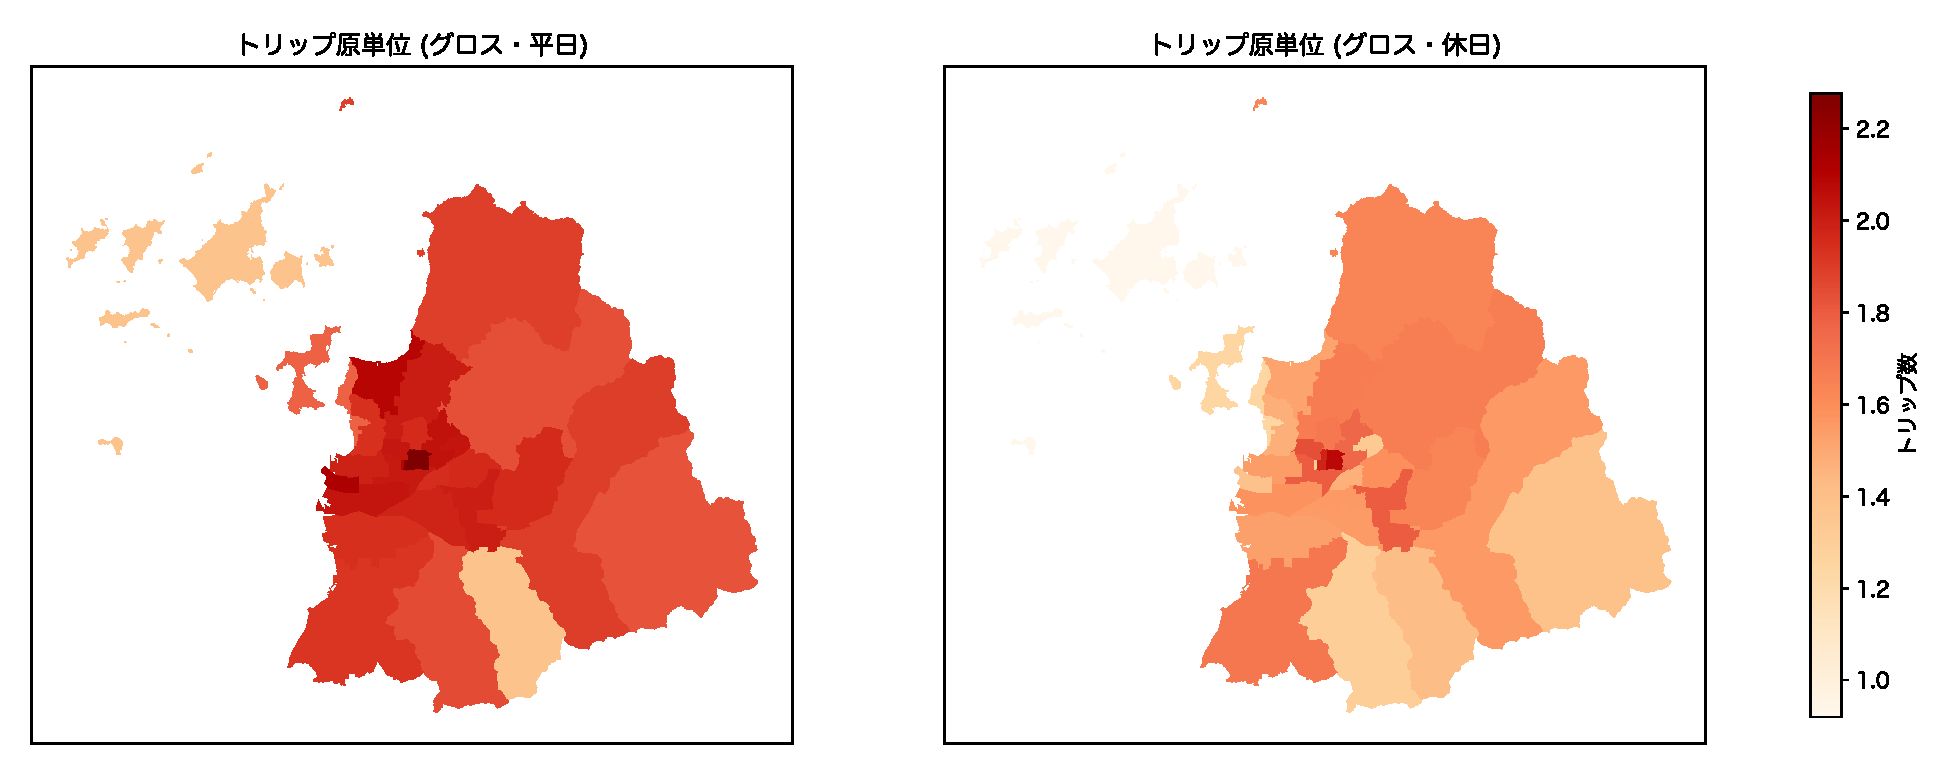
\includegraphics[width=1.0\textwidth]{picture/トリップ数_全体.eps}
    \caption{地域別のトリップ原単位 (グロス)}
    \label{fig:generation_all}
\end{figure}

\begin{figure}[htbp]
    \centering
    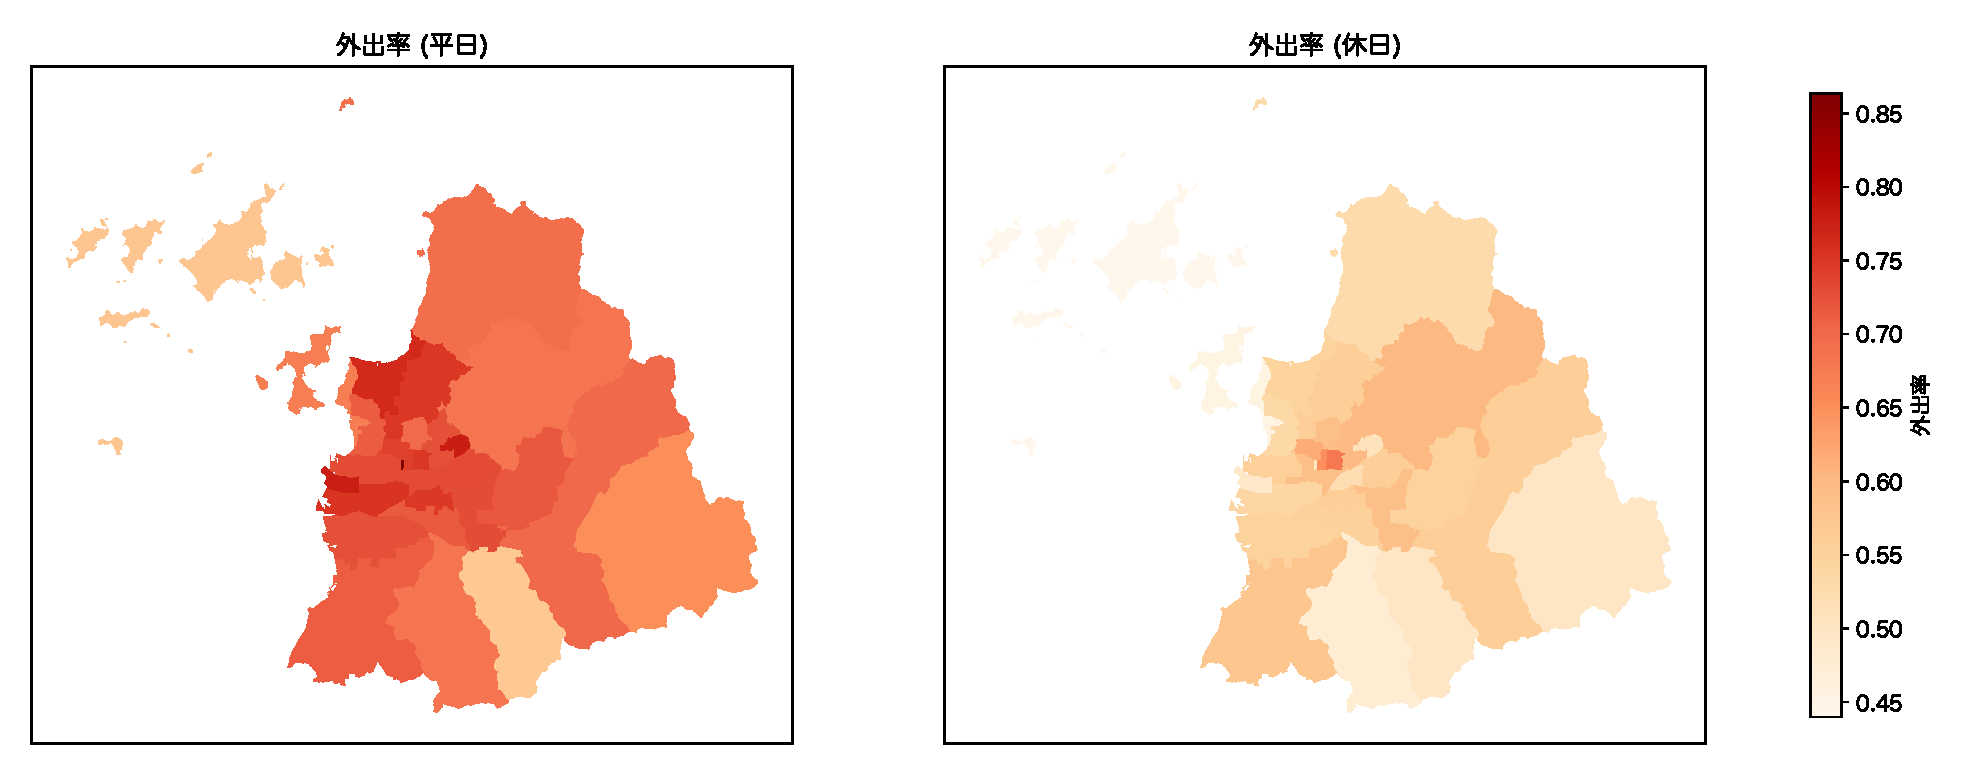
\includegraphics[width=1.0\textwidth]{picture/外出率_全体.eps}
    \caption{地域別の外出率}
    \label{fig:out_all}
\end{figure}

\clearpage
\subsection{性・年齢別の傾向}
次に、性年齢別のトリップ原単位と外出率を、図\ref{fig:generation_gender_age}, 図\ref{fig:out_gender_age}, 図\ref{fig:generation_gender_age_net}に示す。

人口全体のトリップ原単位 (グロス。図\ref{fig:generation_gender_age})は、19-22歳の大学生年代で低く、平日で1.85-1.96、休日で1.18-1.29である。
その後、平日・休日ともに40歳代・50歳代をピークとして上昇し、70歳代以降に急激に減少する。
特に注目すべき点に、19-22歳の大学生年代の休日のトリップ原単位が、70歳代より小さいことが挙げられる。

この原因は、外出率の低下と外出する人のトリップ数の減少によって説明できる。
図\ref{fig:out_gender_age}の性年齢別の外出率によると、19-29歳の若年層の平日の外出率は、女性が76-82\%と他の年代と比較して大きい一方、男性は75-76\%と30-50歳代の外出率に比べて小さく、60歳代の外出率と同程度である。
また、休日の外出率は、19-22歳の男性が45\%、女性が49\%と70歳代 (男性57\%、女性51\%)より低い。

図\ref{fig:generation_gender_age_net}に示す、外出した人の1日の平均トリップ数 (ネット原単位)によれば、平日のネット原単位は、29歳以下の年代で他の年代と比較して男女ともに小さい。
また、休日のネット原単位も、19-29歳は30-60歳代と比べて小さく、特に19-22歳の大学生年代は70歳代と同水準である。

性別差に着目すると、20歳代までは男女の外出率は同程度か女性の方が少し大きいが、30歳代以降は男性の外出率の方が大きく、その差は高齢になるほど拡大する。
ネット原単位は、30-50歳代で女性のネット原単位が大きい。
これは、女性の買い物トリップにより、外出する人の平均トリップ数が大きいと推察される。
その他の年代では、男女で同程度か、男性の方が少し大きい。

\begin{figure}[htbp]
    \centering
    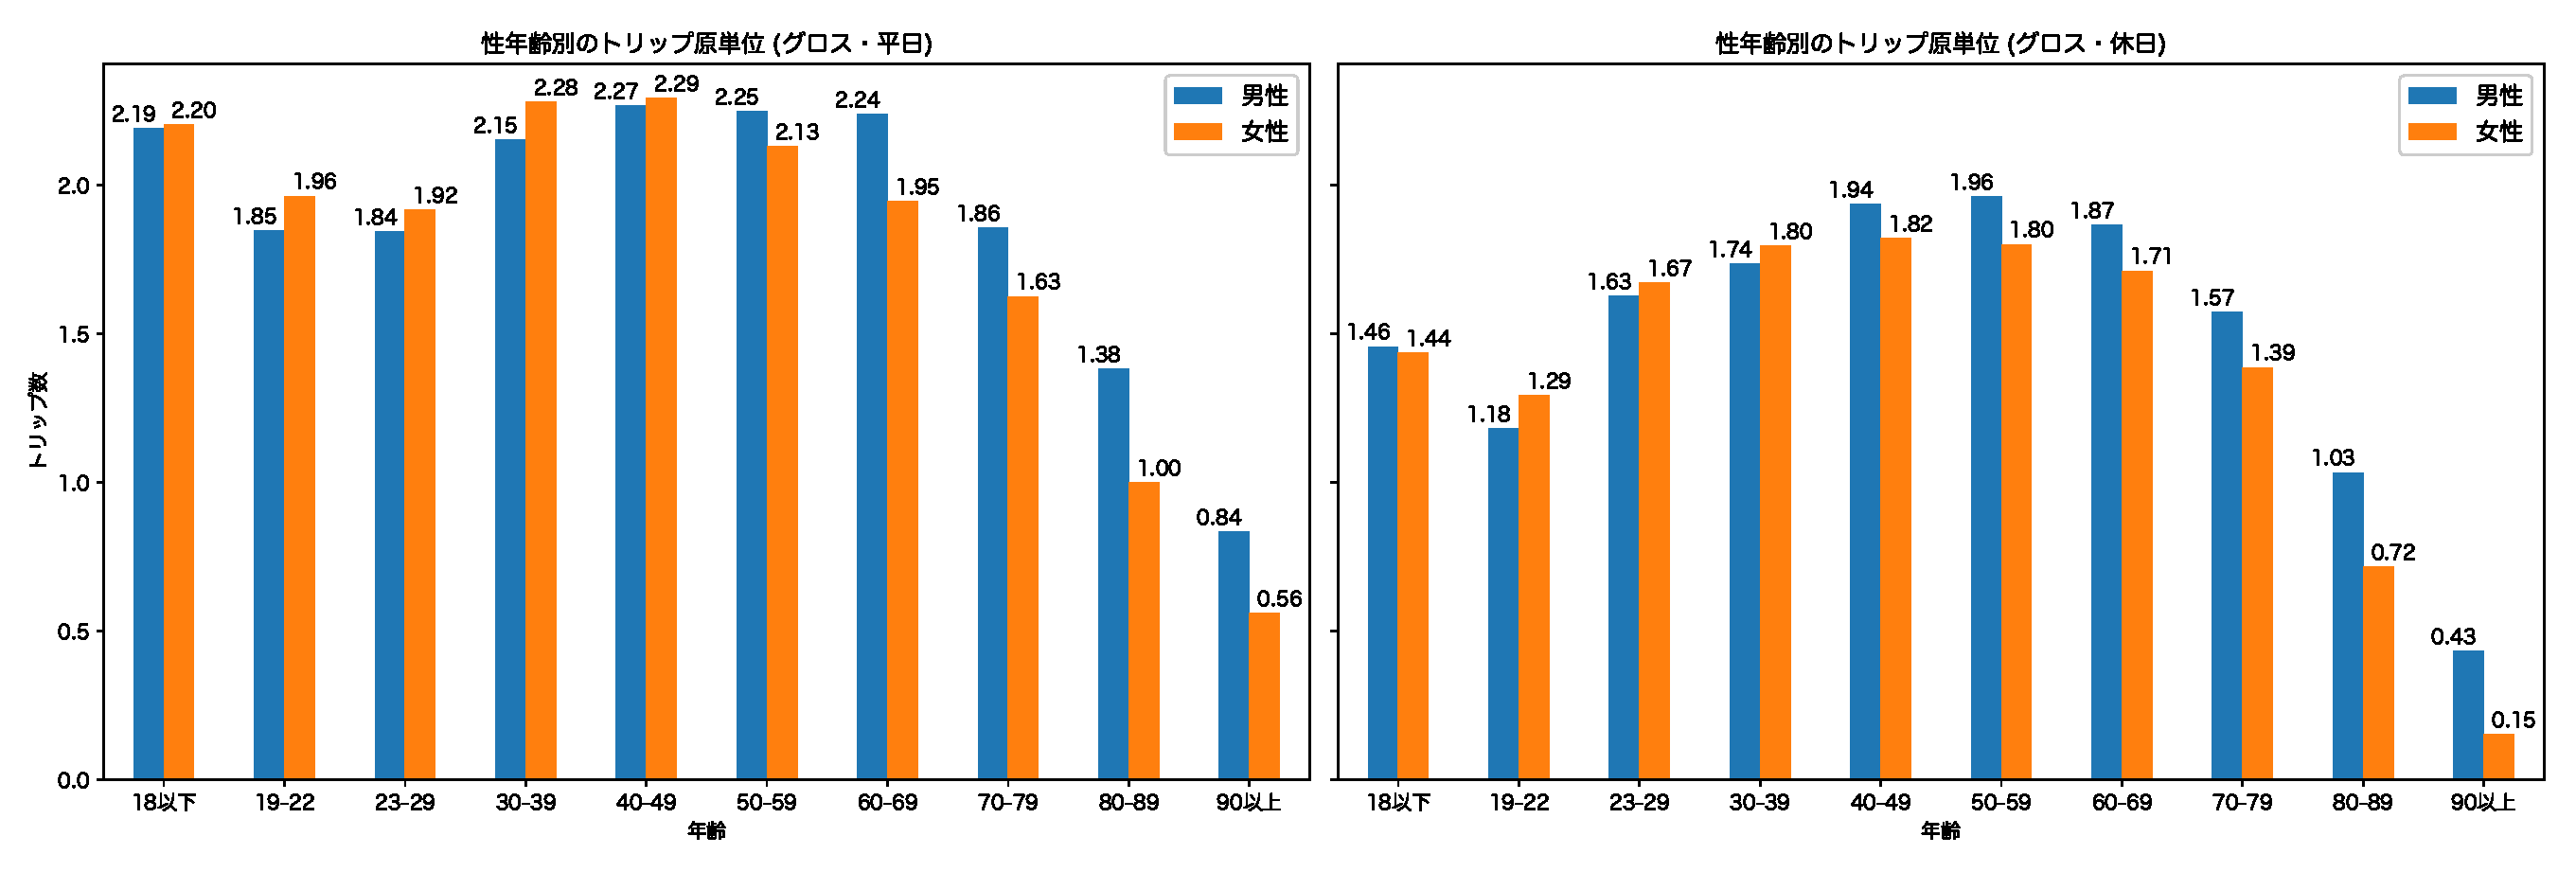
\includegraphics[width=1.0\textwidth]{picture/性年齢別のトリップ数.eps}
    \caption{性年齢別のトリップ原単位 (グロス)}
    \label{fig:generation_gender_age}
\end{figure}

\begin{figure}[htbp]
    \centering
    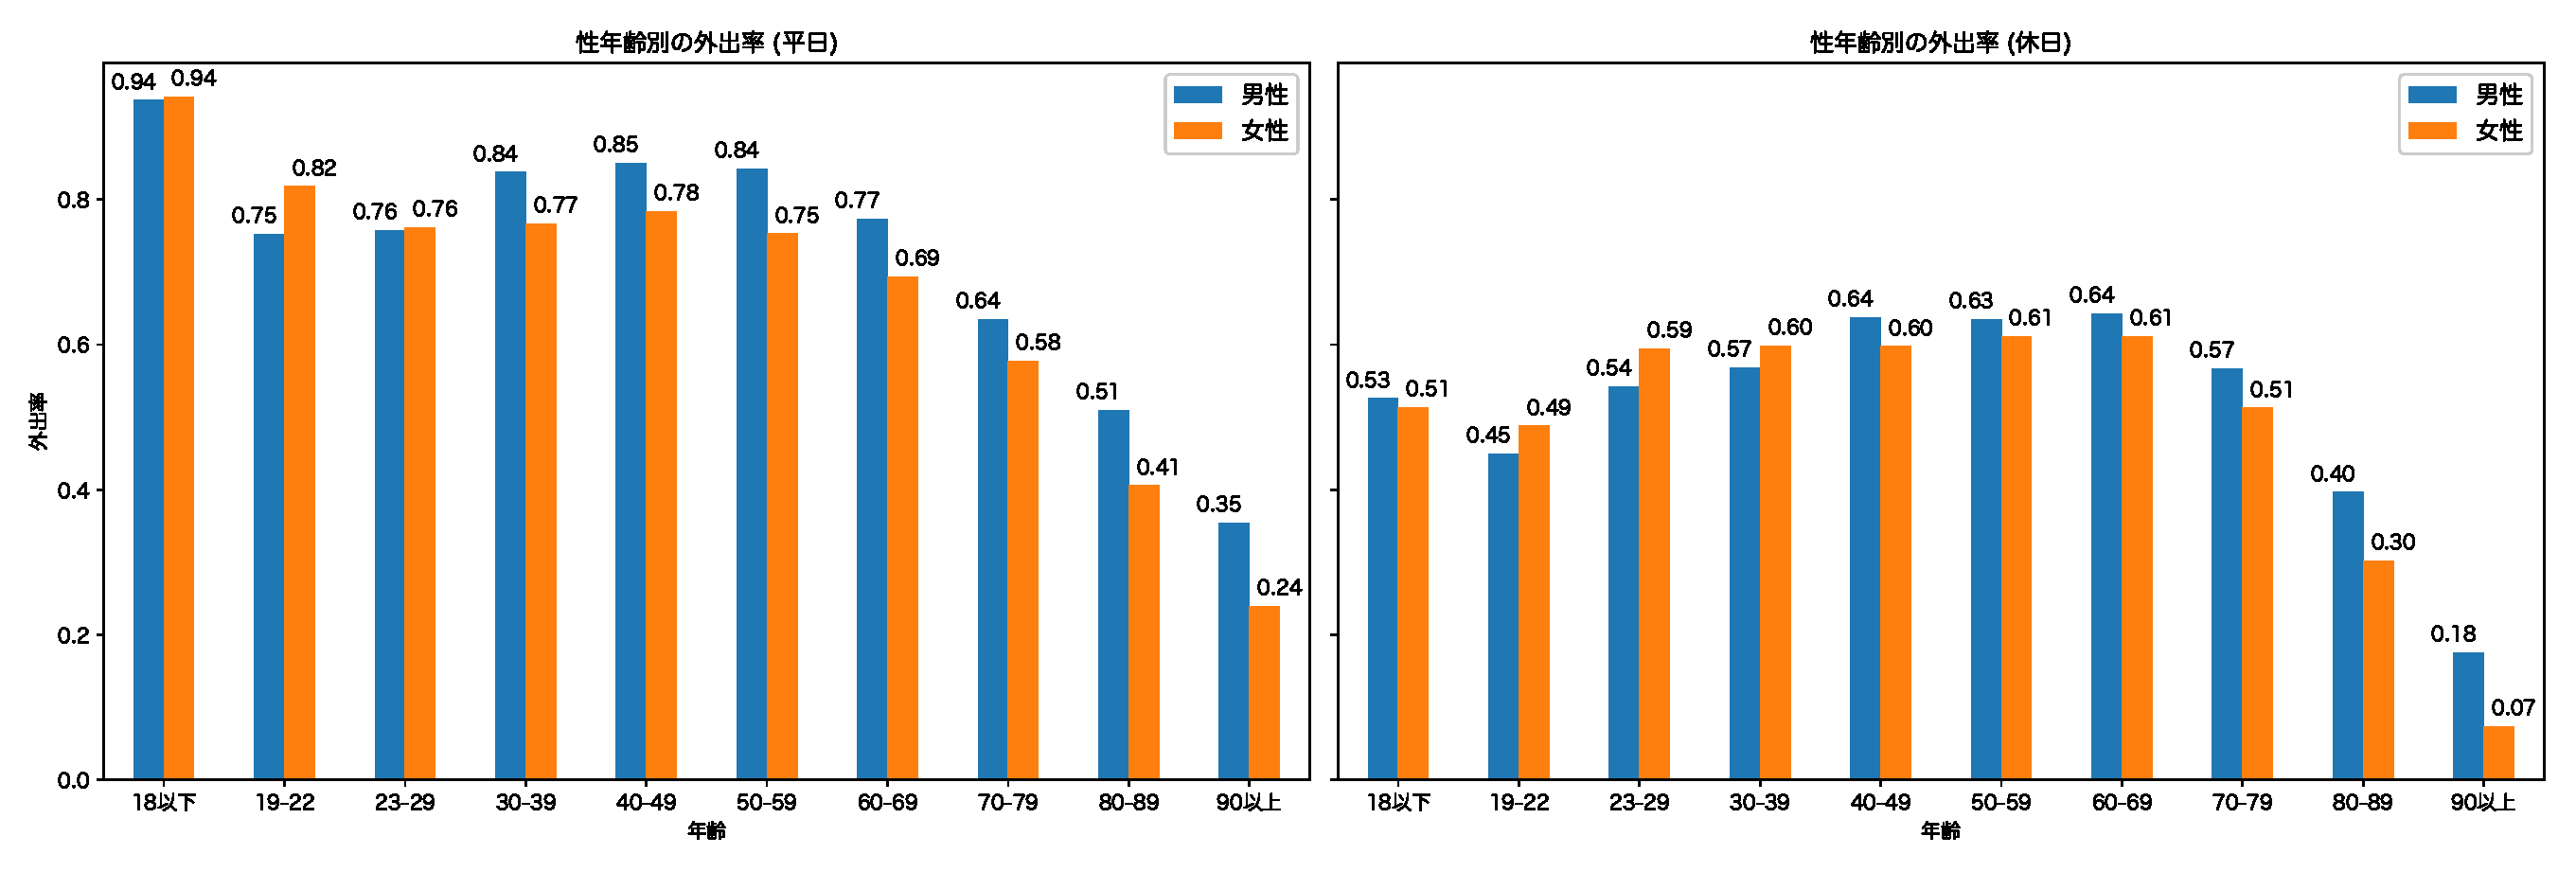
\includegraphics[width=1.0\textwidth]{picture/性年齢別の外出率.eps}
    \caption{性年齢別の外出率}
    \label{fig:out_gender_age}
\end{figure}

\begin{figure}[htbp]
    \centering
    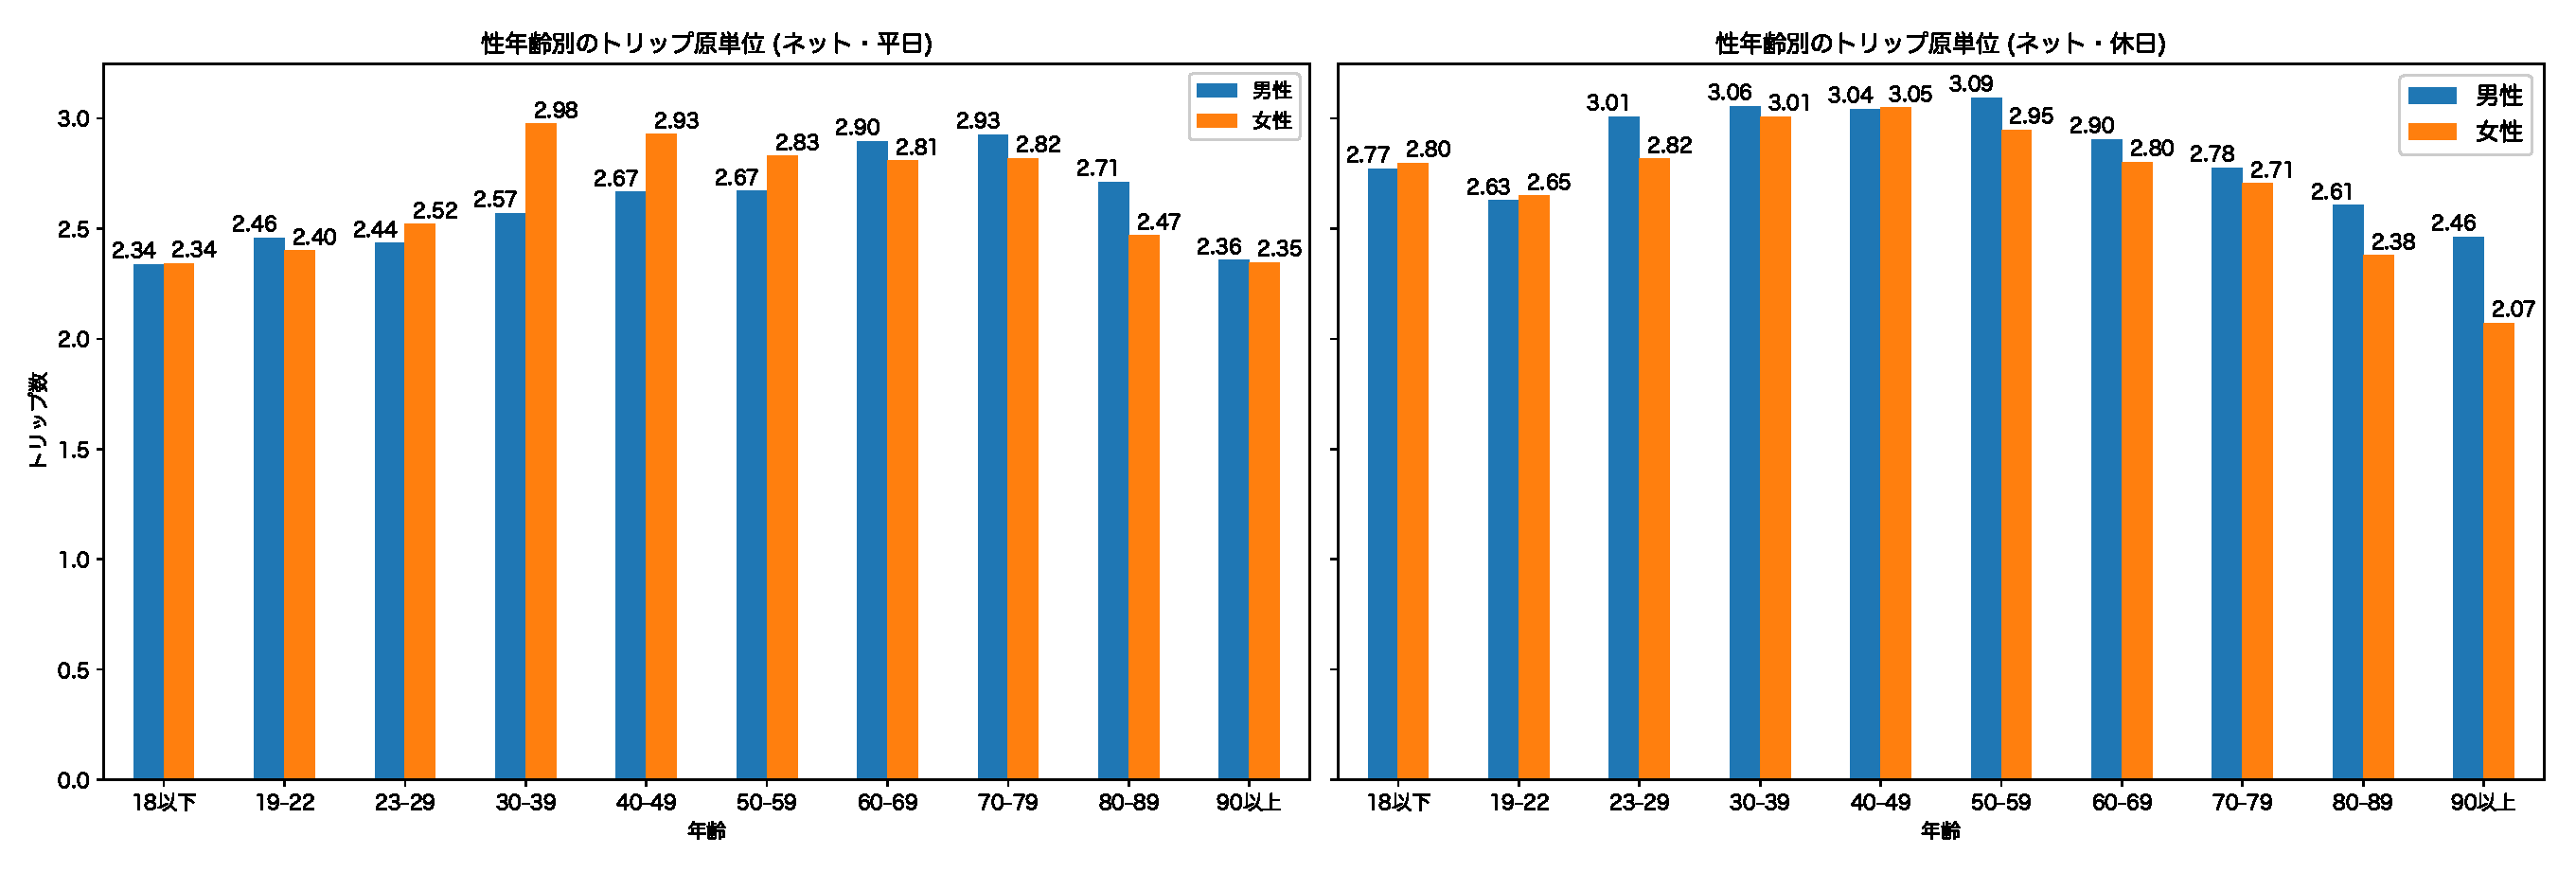
\includegraphics[width=1.0\textwidth]{picture/性年齢別のトリップ数_ネット.eps}
    \caption{性年齢別のトリップ原単位 (ネット)}
    \label{fig:generation_gender_age_net}
\end{figure}

以上で観察された傾向を、過去のデータや他の都市と比較する。
図\ref{fig:out_generation_2007}に、2007年松山都市圏パーソントリップ調査の結果を示す。
これによれば20歳代のネット原単位 (外出した人のみの1日の平均トリップ数)やグロス原単位 (外出していない人も含む1日の平均トリップ数)は、他の年代と比較して小さく、ネット原単位は70歳代を下回る。
この傾向は、今回調査の傾向と一致する。
一方で、2007年調査における、20歳代の外出率は30-60歳代と同程度であり、2023年調査の20歳代の外出率の著しい低下は、これまでに見られなかった現象であると言える。

図\ref{fig:out_generation_sendai}に、2017年仙台都市圏パーソントリップ調査の結果を示す。
トリップ原単位 (グロス)は、20歳代は他の年代と比較して低い傾向にあり、これは本調査での傾向と一致する。
一方で、20歳代の外出率は30-60歳代と同程度で、松山都市圏の外出率より10\%程度高い。
よって、松山都市圏における若年層の外出率の低下が、他の都市と比較しても顕著な現象であると言える。

\begin{comment}
\begin{figure}[htbp]
  % 最初の図---------------------------
  \begin{minipage}[b]{0.55\textwidth}
    \centering
    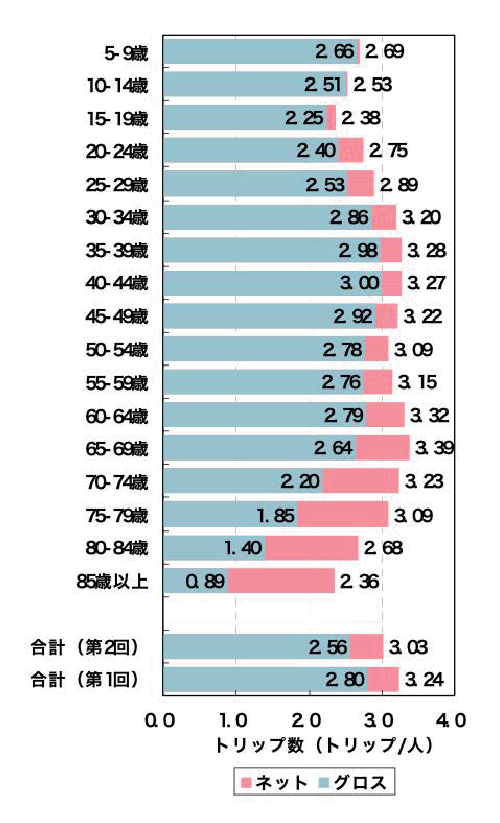
\includegraphics[scale=0.7]{picture/gross_net_2007.eps}
    \subcaption{トリップ原単位}
  \end{minipage}
  % 2番目の図--------------------------
  \begin{minipage}[b]{0.35\textwidth}
    \centering
    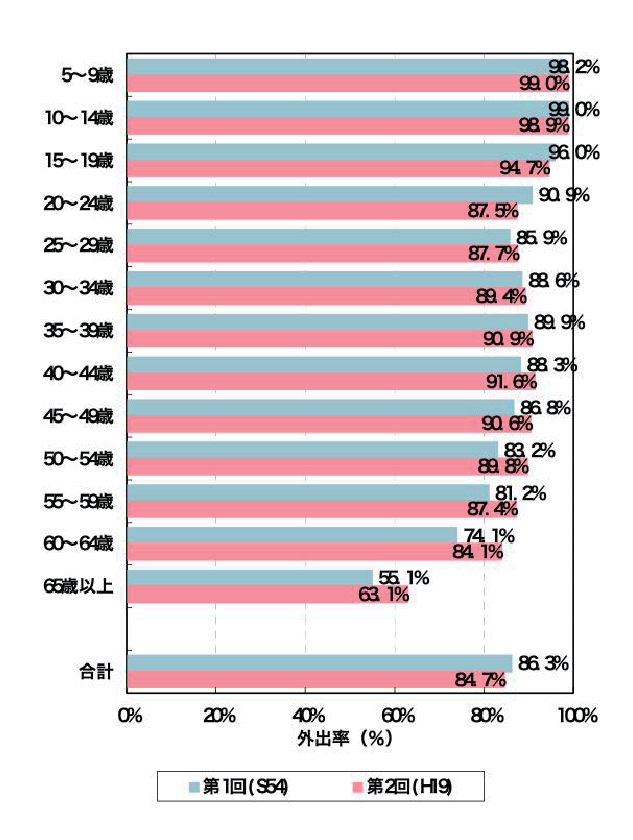
\includegraphics[scale=0.7]{picture/out_2007.eps}
    \subcaption{外出率}
  \end{minipage}
  \caption{2007年松山都市圏パーソントリップ調査\cite{松山市総合交通戦略}}
  \label{fig:out_generation_2007}
\end{figure}
\end{comment}

\begin{figure}[htbp]
  \centering
	\subfigure[トリップ原単位]{%
		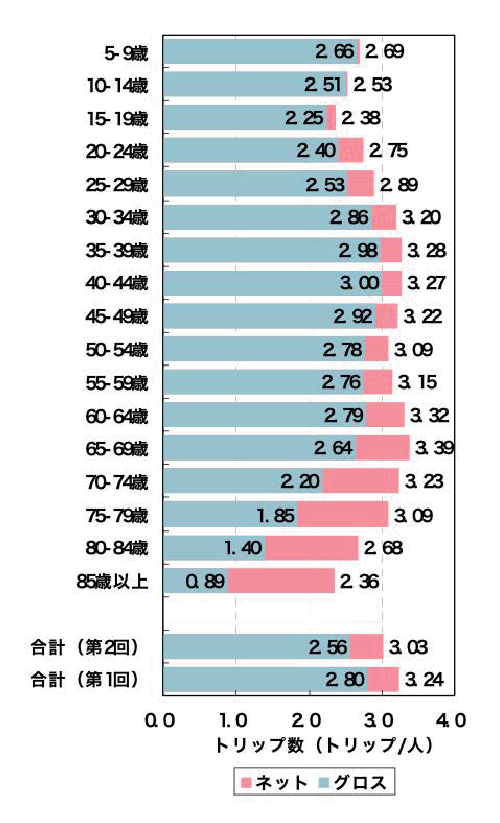
\includegraphics[clip, width=0.32\columnwidth]{picture/gross_net_2007.eps}}%
	\subfigure[外出率]{%
		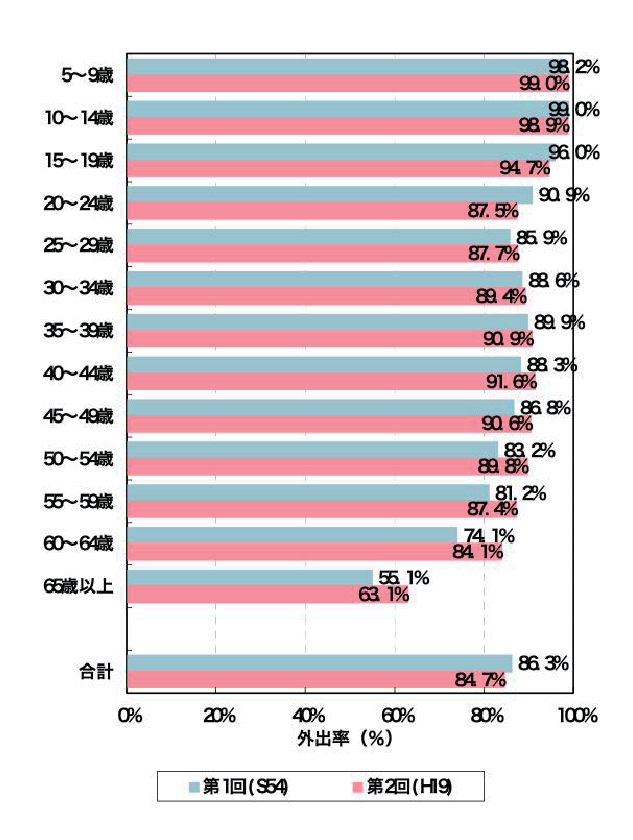
\includegraphics[clip, width=0.4\columnwidth]{picture/out_2007.eps}}%
	\caption{2007年松山都市圏パーソントリップ調査\cite{松山市総合交通戦略}}
	\label{fig:out_generation_2007}
\end{figure}

\begin{figure}[htbp]
  \centering
	\subfigure[トリップ原単位 (グロス)]{%
		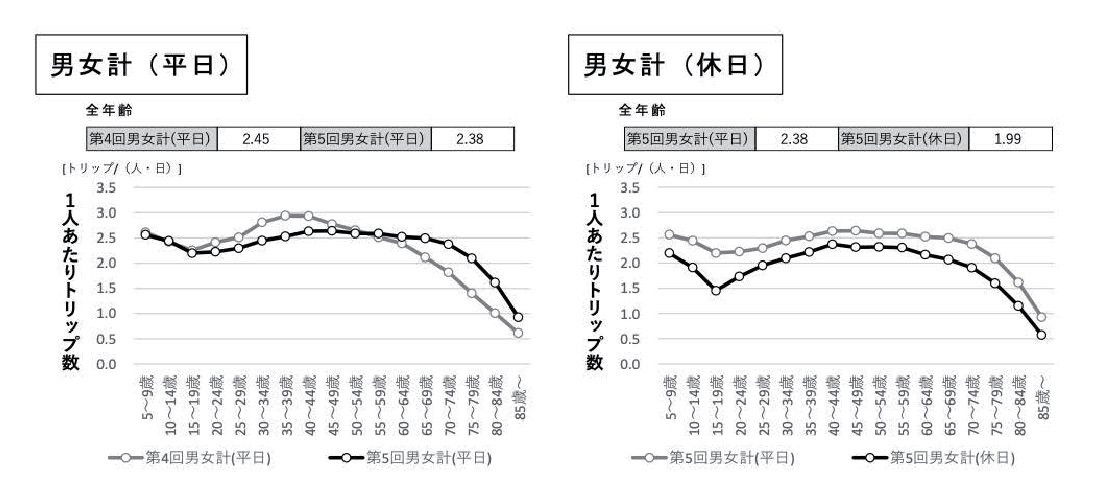
\includegraphics[clip, width=0.75\columnwidth]{picture/gross_sendai.eps}} \\ %
	\subfigure[外出率]{%
		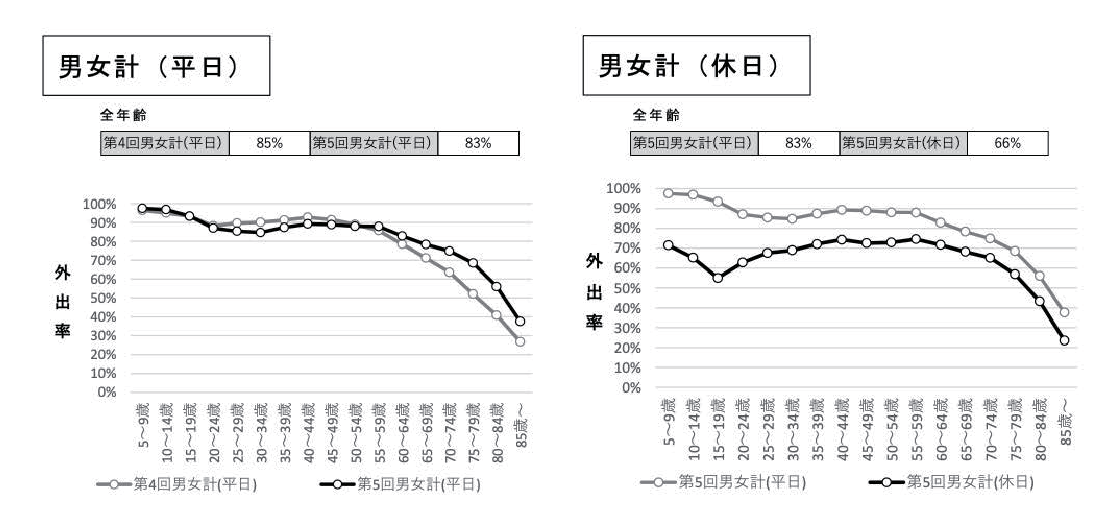
\includegraphics[clip, width=0.75\columnwidth]{picture/out_sendai.eps}}%
	\caption{2017年仙台都市圏パーソントリップ調査\cite{sendai}}
	\label{fig:out_generation_sendai}
\end{figure}

\color{red}
\begin{framed}
\noindent
\textbf{\large 20歳代の若年層の移動が、過去の調査や他都市の調査に比べて少ない。これは、若年層の休日の外出率が低いことと、外出する人のトリップ数が少ないことに起因する。}
\end{framed}
\color{black}


\clearpage
\section{トリップの出発地と到着地の分析}
\subsection{通勤・通学}
図\ref{fig:od_commute}は、通勤・通学のトリップの出発地 (左列)と到着地 (右列)の関係を表し、線の幅はトリップ数を表す。
通勤・通学トリップは、松山市1区 (市駅、大街道、松山城)、松山市3区 (愛媛大、松山東高、祝谷)、松山市5区 (土橋、空港通、南江戸)のエリアに集中しており、職場や学校が集中している。
また、このようなエリアに向けてトリップが多く出発するエリアは、松山市5区 (土橋、空港通、南江戸)、松山市7区 (木屋町、山越、姫原)、松山市10区 (桑原、畑寺、東野)、松山市15区 (垣生、余戸、土居田)が多く、都市近郊の住宅街としての役割を果たしていると考えられる。

一方で、砥部町、東温市、伊予市、松前町、北条地域は域内の移動が主であり、行政界や地域を跨いだ移動は、
\begin{enumerate}
  \item 松前町と伊予市・松山市15区 (垣生、余戸、土居田)
  \item 東温市と松山市9区 (平井、梅本、東久米)、松山市11区 (久米、南土居、高井)
  \item 北条と和気・堀江、
\end{enumerate}
を除いてほとんどない。

\begin{figure}[htbp]
    \centering
    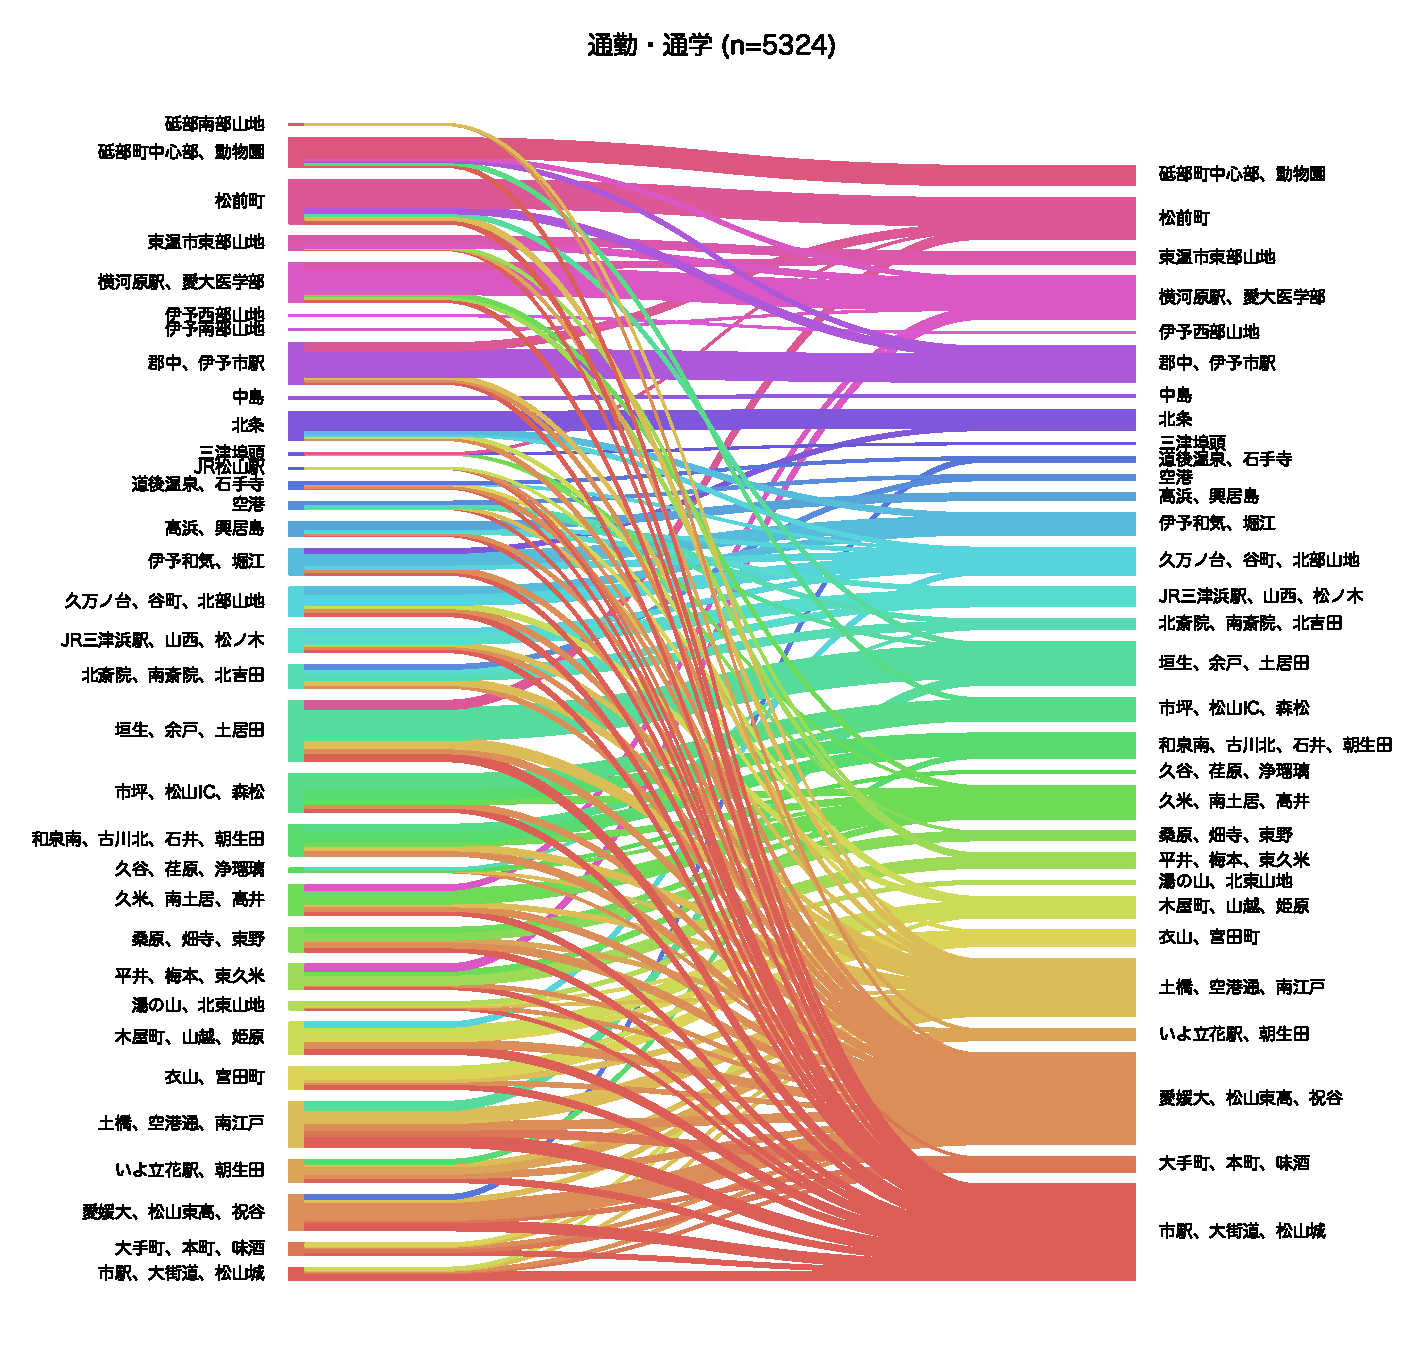
\includegraphics[width=1.0\textwidth]{picture/connection_通勤・通学.eps}
    \caption{通勤・通学の出発地 (左列)と到着地 (右列)}
    \label{fig:od_commute}
\end{figure}

\color{red}
\begin{framed}
\noindent
\textbf{\large 通勤・通学の移動は、松山市郊外の住宅地から松山市駅・松山城周辺エリアに向けた移動が主である。砥部町、東温市、伊予市、松前町、北条地域は、近隣の地区との行き来はあるものの、域内の移動が主である。}
\end{framed}
\color{black}

\clearpage
\subsection{買い物}
図\ref{fig:od_shopping}は、買い物のトリップの出発地 (左列)と到着地 (右列)の関係を表し、線の幅はトリップ数を表す。
買い物トリップは、松山市6区 (衣山、宮田町)、松山市13区 (和泉南、古川北、石井、朝生田)、松山市15区 (垣生、余戸、土居田)、東温市1区 (横河原駅、愛大医学部)、松前町、伊予市1区 (郡中、伊予市駅)のエリアに集中しており、郊外のショッピングセンターや国道周辺のロードサイド店舗への買い物が多いと考えられる。

特に、松山市6区 (衣山、宮田町)、松山市13区 (和泉南、古川北、石井、朝生田)、東温市1区 (横河原駅、愛大医学部)、松前町は、周辺地域からの買い物トリップが集中している。
図\ref{fig:shopping_origin}に各地区に買い物に訪れるトリップの出発地の分布を示す。
各地区は、近隣の地区からの買い物トリップを惹きつけており、買い物の地理的な圏域が存在することや、郊外の住宅地から近場のショッピングセンターやロードサイド店舗に買い物に行くという郊外完結型のライフスタイルが見てとれる。

\color{red}
\begin{framed}
\noindent
\textbf{\large 買い物の移動は、郊外の住宅地から近場のショピングセンターやロードサイド店舗に移動する、郊外から郊外の移動が主である。また、通勤・通学と異なり、行政界を跨いだ移動も盛んである。}
\end{framed}
\color{black}

\begin{figure}[htbp]
    \centering
    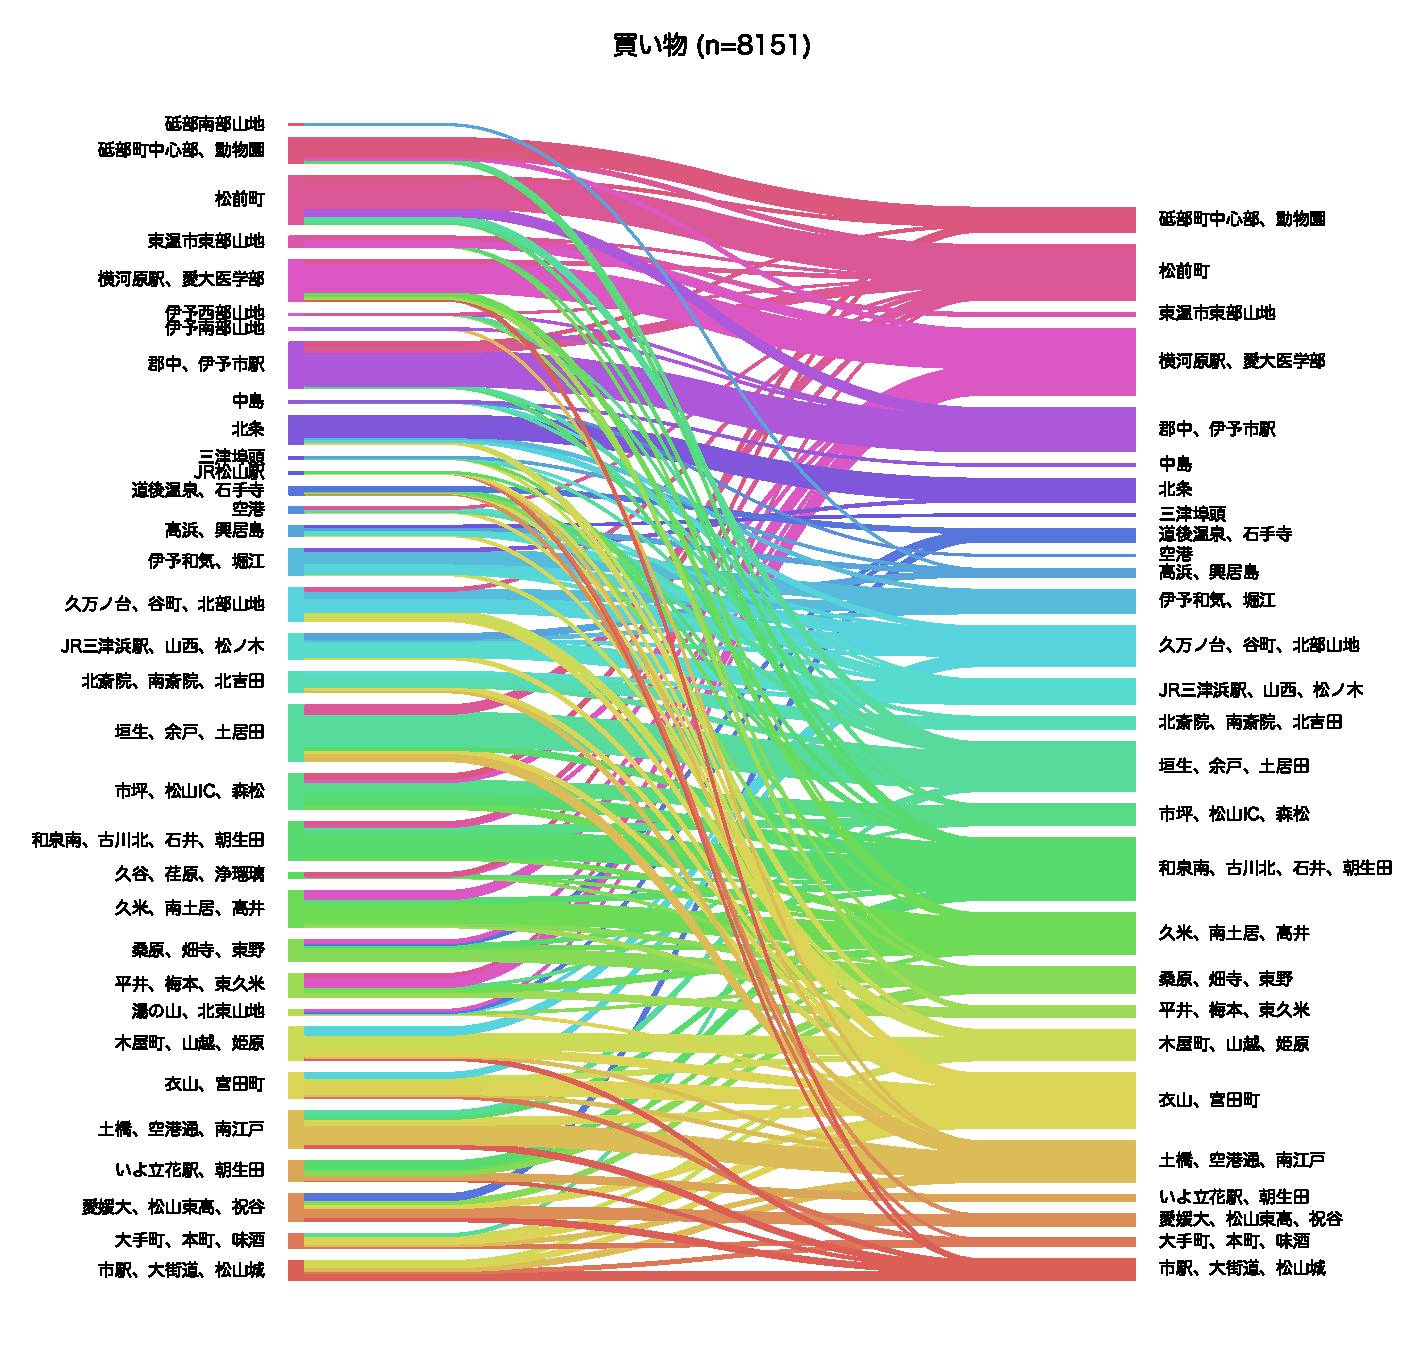
\includegraphics[width=1.0\textwidth]{picture/connection_買い物.eps}
    \caption{買い物の出発地 (左列)と到着地 (右列)}
    \label{fig:od_shopping}
\end{figure}

\begin{figure}[htbp]
	\subfigure[松山市6区 (衣山、宮田町)]{%
		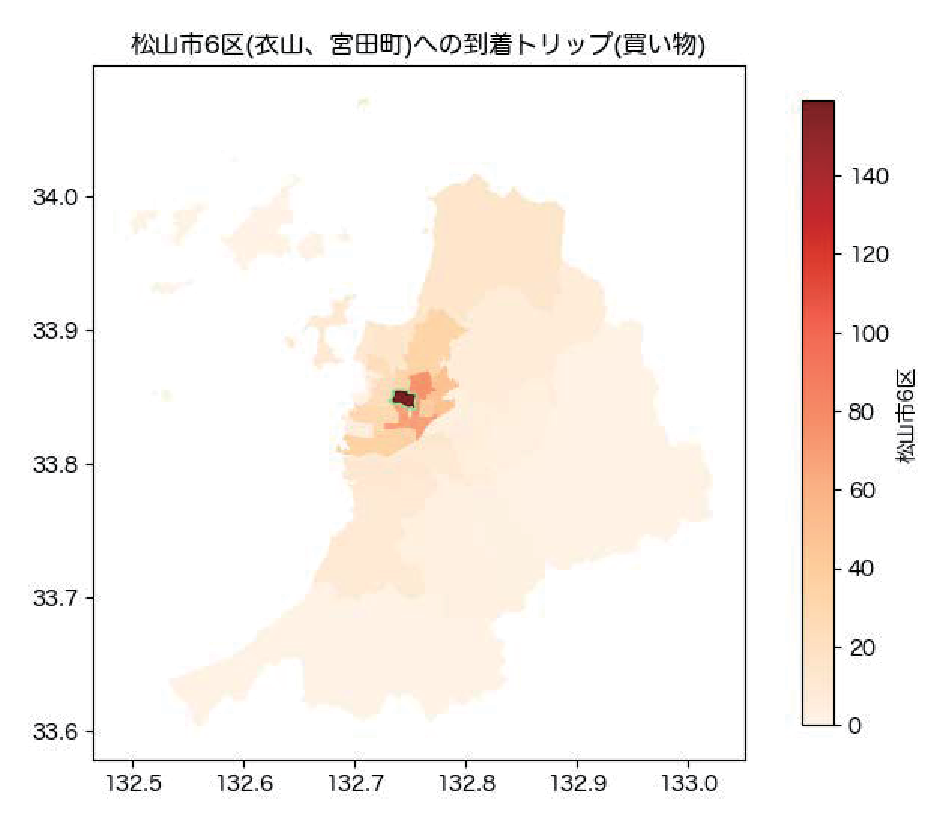
\includegraphics[clip, width=0.45\columnwidth]{picture/shopping_kinuyama.eps}} %
	\subfigure[松山市13区 (和泉南、古川北、石井、朝生田)]{%
		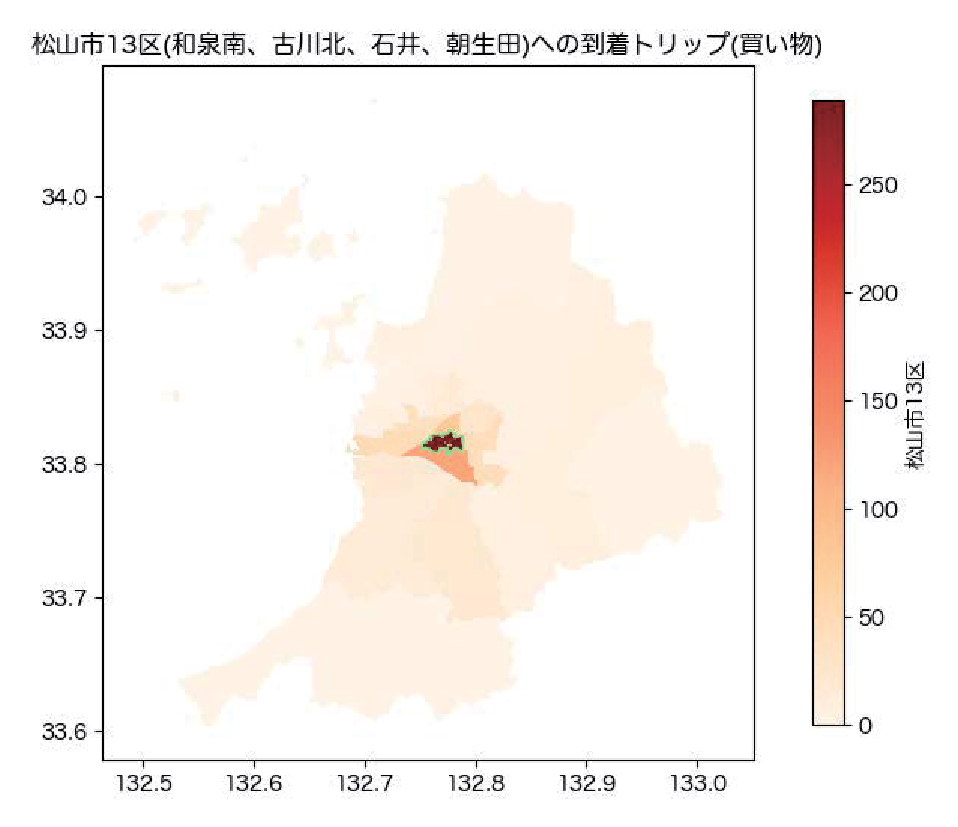
\includegraphics[clip, width=0.45\columnwidth]{picture/shopping_izumi.eps}}%
  \\
  \subfigure[東温市1区 (横河原駅、愛大医学部)]{%
		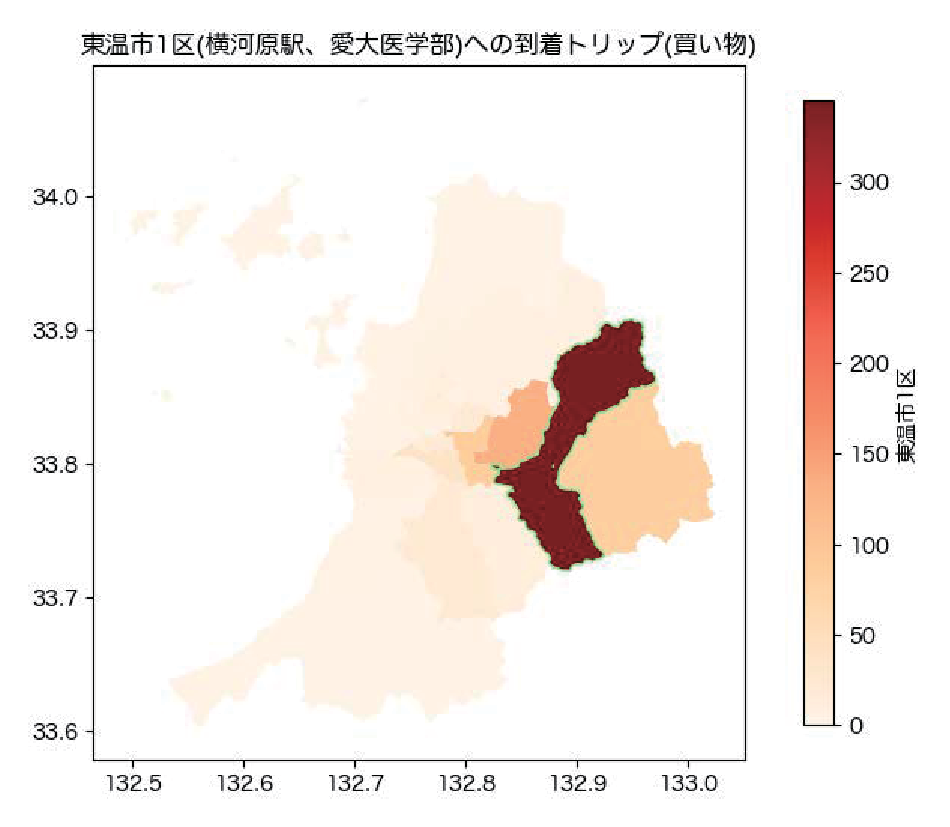
\includegraphics[clip, width=0.45\columnwidth]{picture/shopping_toon.eps}} %
	\subfigure[松前町]{%
		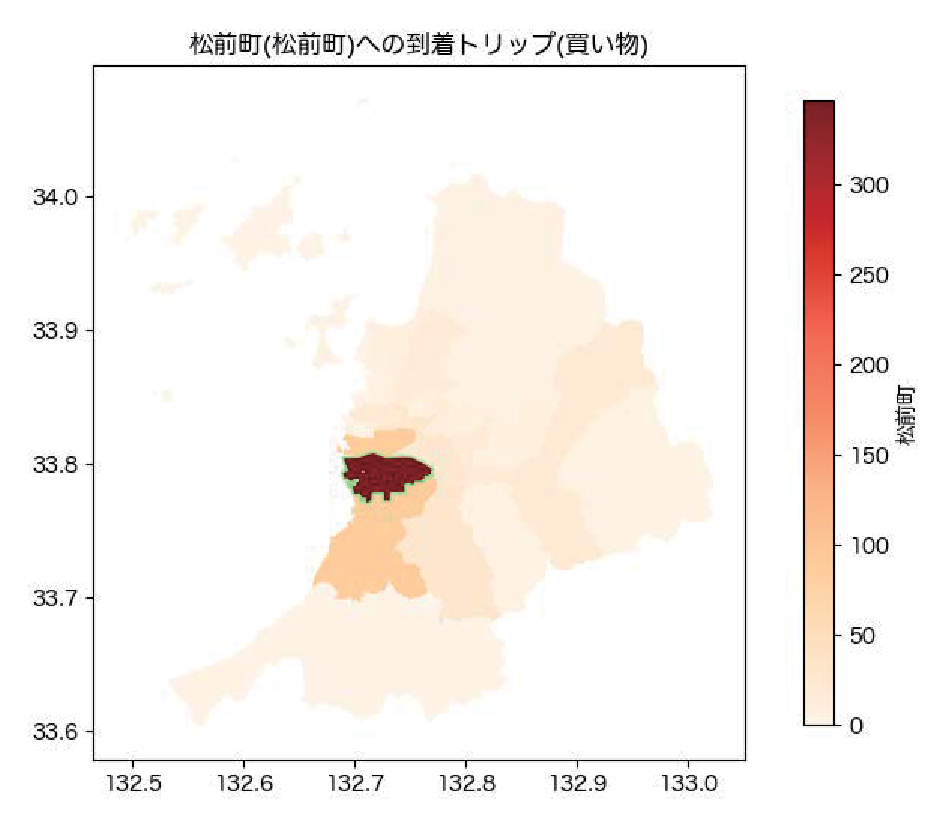
\includegraphics[clip, width=0.45\columnwidth]{picture/shopping_masaki.eps}}%
	\caption{各地区を訪れる買い物トリップの出発地}
	\label{fig:shopping_origin}
\end{figure}


\clearpage
\subsection{食事・社交・娯楽、観光・行楽・レジャー}
図\ref{fig:od_leisure}は、食事・社交・娯楽、観光・行楽・レジャー (まとめて娯楽と呼ぶ)のトリップの出発地 (左列)と到着地 (右列)の関係を表し、線の幅はトリップ数を表す。
娯楽トリップは、松山市1区 (市駅、大街道、松山城)、松山市5区 (土橋、空港通、南江戸)、松山市6区 (衣山、宮田町)、松山市11区 (久米、南土居、高井)、松山市13区 (和泉南、古川北、石井、朝生田)、松山市14区 (市坪、松山IC、森松)、松前町のエリアに集中している。
松山市5区 (土橋、空港通、南江戸)、松山市6区 (衣山、宮田町)、松山市13区 (和泉南、古川北、石井、朝生田)、松前町は、買い物トリップでも周辺地域からのトリップが集中しており、ショッピングセンターやロードサイド店舗での食事・社交・娯楽が買い物と合わせて行われていると考えられる。
松山市5区 (土橋、空港通、南江戸)、地区内に大規模公園があるため、行楽需要が存在すると考えられる。

一方、買い物トリップとの顕著な違いとして、松山市1区 (市駅、大街道、松山城)へのトリップの集中が挙げられる。
松山市1区へ向けて、周辺地域を中心に広範囲から娯楽トリップが集中していることから、中心部の求心性がある程度存在する。
その集中トリップ数は、松山市6区 (衣山、宮田町)や松前町と同程度である。

また、松山市11区 (久米、南土居、高井)、松山市14区 (市坪、松山IC、森松)は、買い物トリップの集中は顕著ではなかったものの、娯楽トリップは比較的多い。
松山市11区 (久米、南土居、高井)は、東温市や松山市9区 (平井、梅本、東久米)等の近隣からの娯楽トリップが多く、松山市14区 (市坪、松山IC、森松)は、松山市15区 (垣生、余戸、土居田)や13区 (和泉南、古川北、石井、朝生田)等の近隣からの娯楽トリップが多い。
これは、地区内の娯楽施設や大規模公園に向けた行楽需要が存在するためと考えられる。

\color{red}
\begin{framed}
\noindent
\textbf{\large 娯楽の移動は、郊外のショピングセンターやロードサイド店舗に加えて、松山市中心市街地、郊外の公園や娯楽施設を目的地とするトリップが多い。}
\end{framed}
\color{black}

\begin{figure}[htbp]
    \centering
    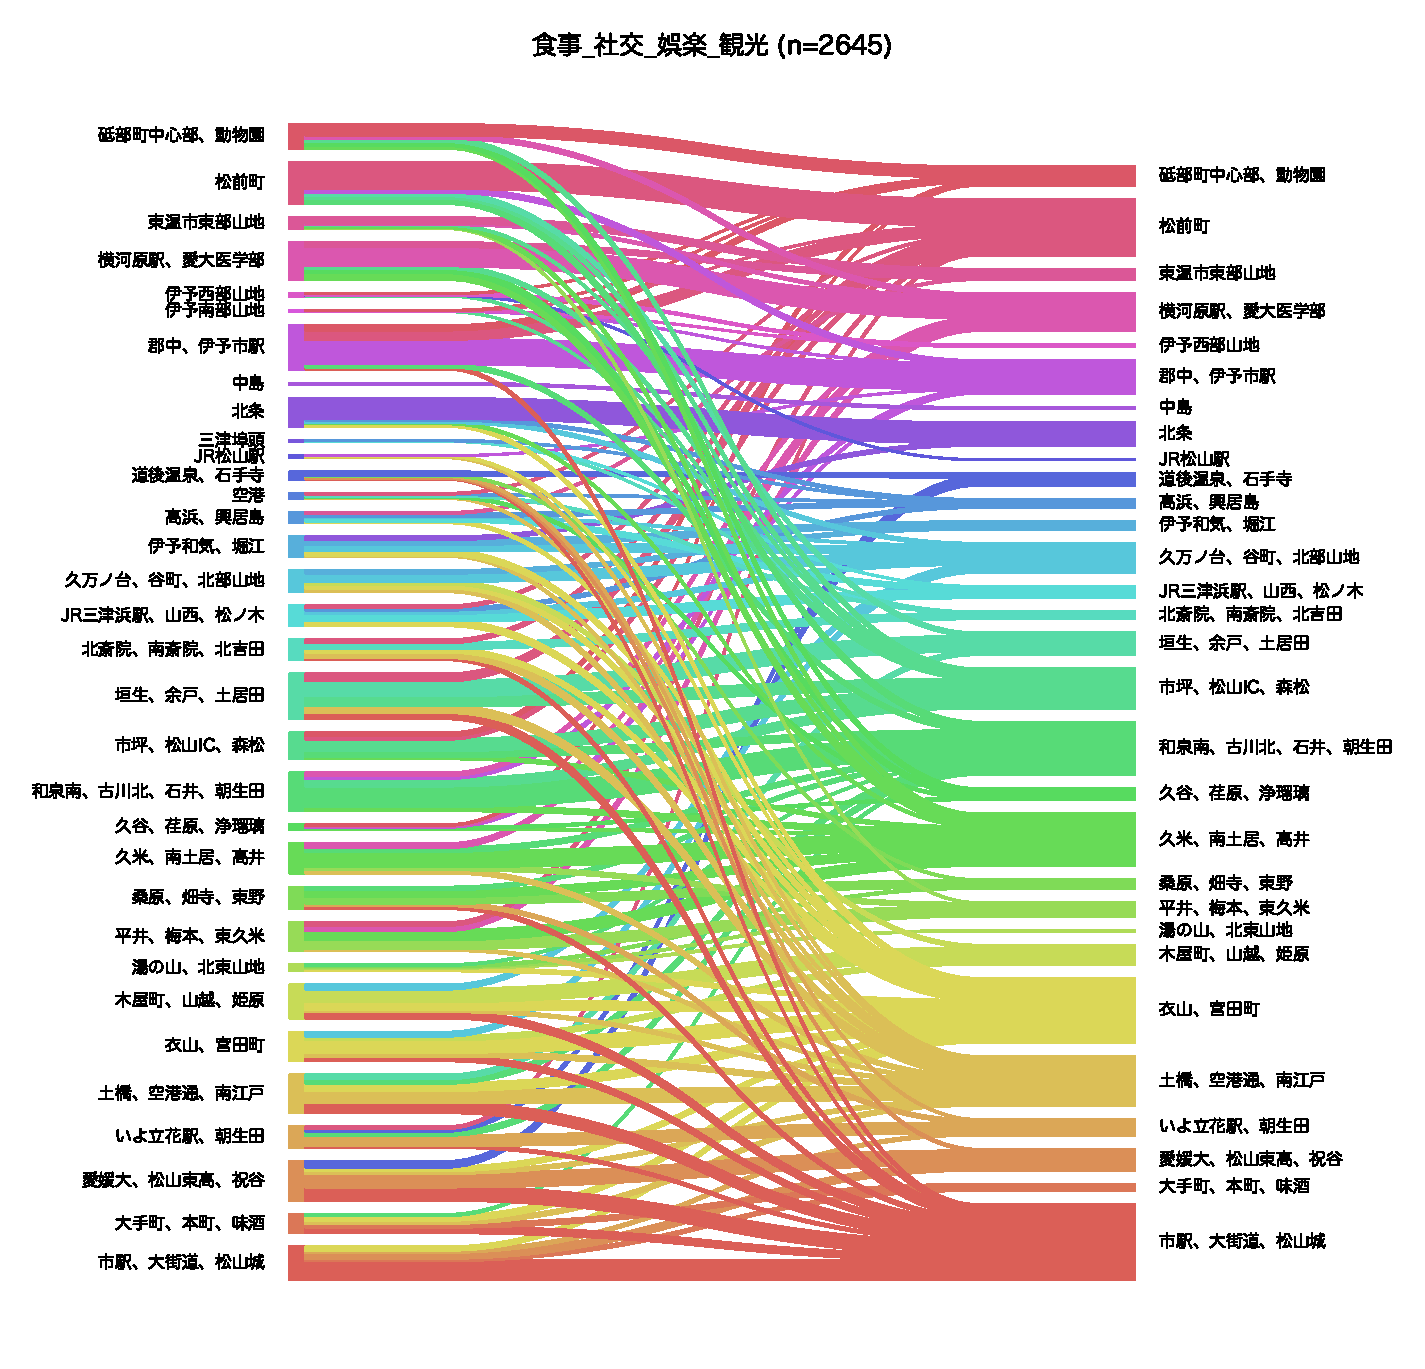
\includegraphics[width=1.0\textwidth]{picture/connection_食事_社交_娯楽_観光.eps}
    \caption{食事・社交・娯楽・観光の出発地 (左列)と到着地 (右列)}
    \label{fig:od_leisure}
\end{figure}


%\clearpage
%\subsection{ポイントデータの分析}
%ヒートマップ


\clearpage
\section{交通手段分担率の分析}
\subsection{全体的な傾向}
図\ref{fig:mode_share}に全トリップの交通手段分担率を示す。
代表交通手段の優先順位は、鉄道、路面電車、バス、自動車、タクシー、原付・二輪、自転車、徒歩である。
自動車交通が、平日は59\%、休日は70\%を占めており、車社会が形成されている。
徒歩と自転車は、合わせて平日は27\%、休日は21\%を占めるが、バス・鉄道・路面電車の占める割合は、2〜5\%にすぎない。
特に、休日の方が自動車交通の占める割合が高く、休日に行われる買い物や娯楽活動に自動車が多く用いられていることが推測される。

\begin{figure}[htbp]
    \centering
    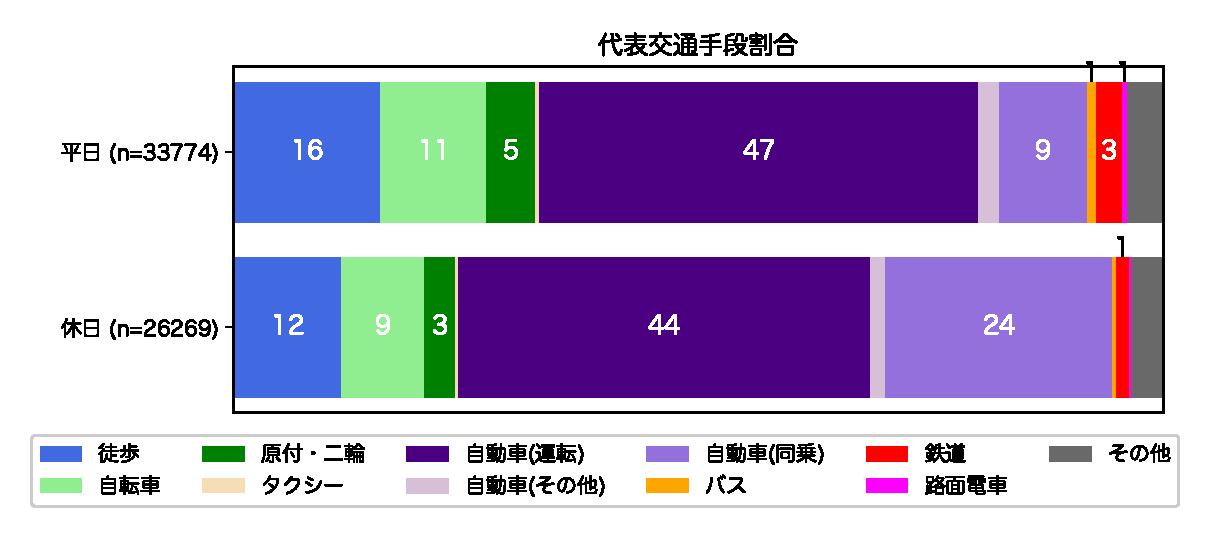
\includegraphics[width=1.0\textwidth]{picture/mode_share_day.eps}
    \caption{交通手段分担率}
    \label{fig:mode_share}
\end{figure}

公共交通機関によるトリップの平均移動距離は、12.51kmである。
出発地として多いのは、
\begin{comment}
\begin{enumerate}
  \item 松山市1区 (市駅、大街道、松山城)
  \item 松山市3区 (愛媛大、松山東高、祝谷)
  \item 松山市15区 (垣生、余戸、土居田)
  \item 松山市5区 (土橋、空港通、南江戸)
  \item 松山市6区 (衣山、宮田町)
\end{enumerate}

到着地として多いのは、
\begin{enumerate}
  \item 松山市1区 (市駅、大街道、松山城)
  \item 松山市3区 (愛媛大、松山東高、祝谷)
  \item 松山市6区 (衣山、宮田町)
  \item 松山市15区 (垣生、余戸、土居田)
  \item 松山市5区 (土橋、空港通、南江戸)
\end{enumerate}
\end{comment}

次に、この結果を他都市や過去の調査と比較する。
図\ref{fig:mode_past},図\ref{fig:mode_kumamoto}, 図\ref{fig:mode_sendai}は、それぞれ、過去の松山都市圏パーソントリップ調査、2023年熊本都市圏パーソントリップ調査\cite{kumamoto}、2017年仙台都市圏パーソントリップ調査\cite{sendai}の交通手段分担率である。
過去の調査と比較して、松山都市圏において自動車依存度は増している。
2023年調査の全体の自動車分担率は63.9\%で、2007年度調査に比べて、13\%増加した。
その分、自転車の分担率がおよそ10\%、徒歩の分担率がおよそ3\%低下している。

仙台、熊本と比較すると、分担率の構成は概ね同じである。
一方で、熊本と比較すると、バス・徒歩・自転車の分担率が若干低く、仙台と比較すると、鉄道とバスの分担率が若干低い。
よって、松山も他の地方都市と同様に自動車依存社会の問題を抱えていると言える。

\begin{figure}[htbp]
    \centering
    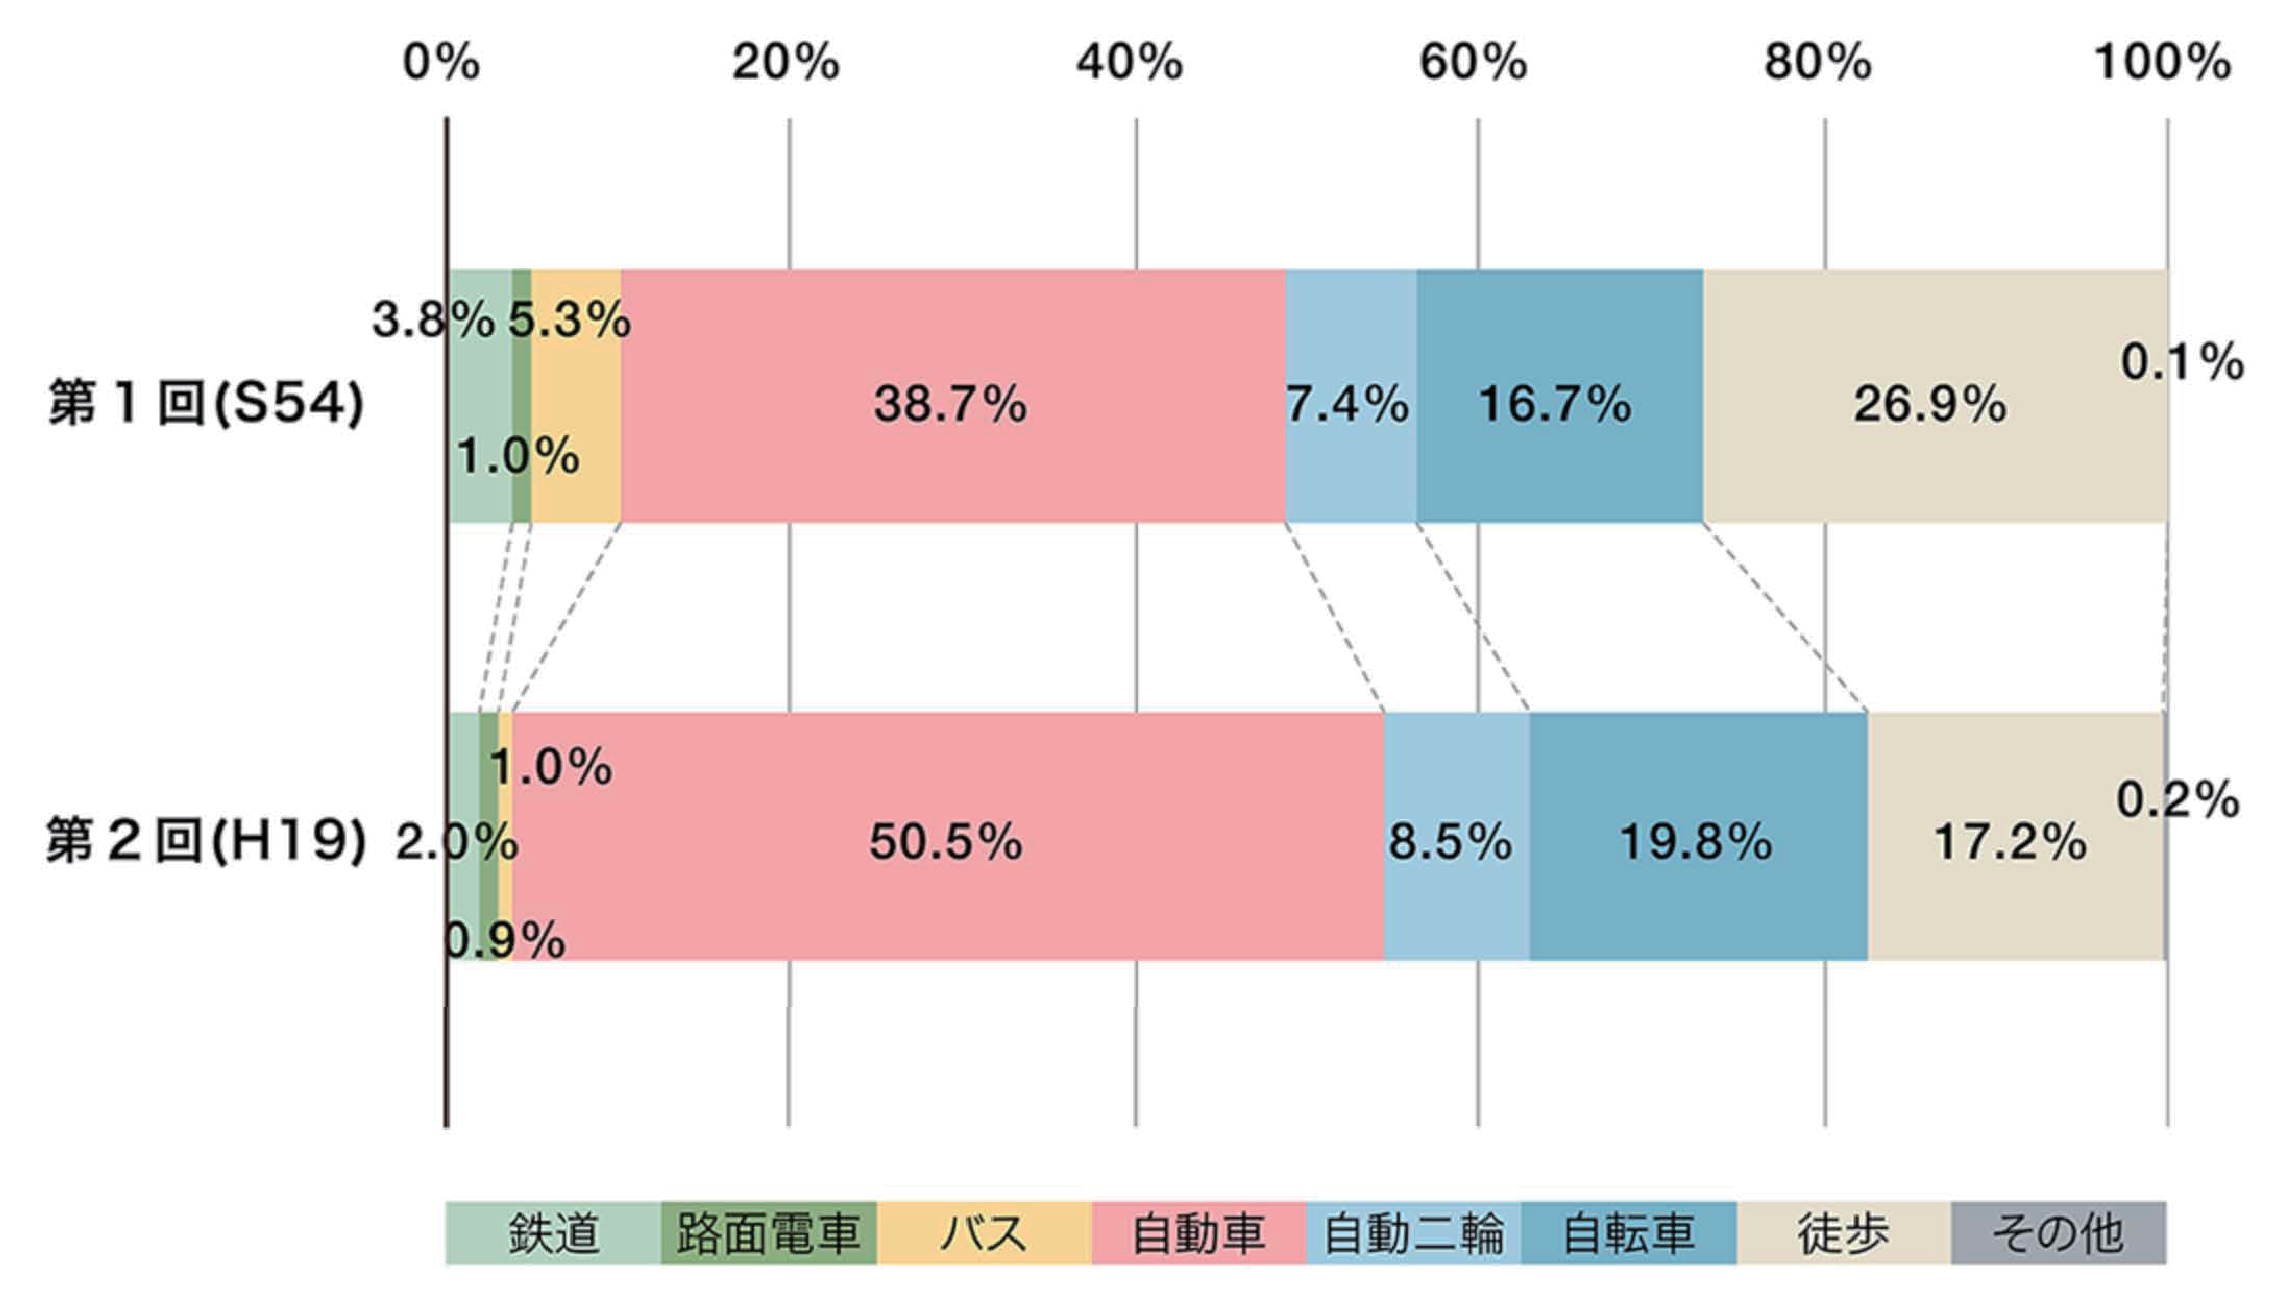
\includegraphics[width=0.8\textwidth]{picture/mode_past.eps}
    \caption{過去の松山都市圏パーソントリップ調査の交通手段分担率}
    \label{fig:mode_past}
\end{figure}

\begin{figure}[htbp]
    \centering
    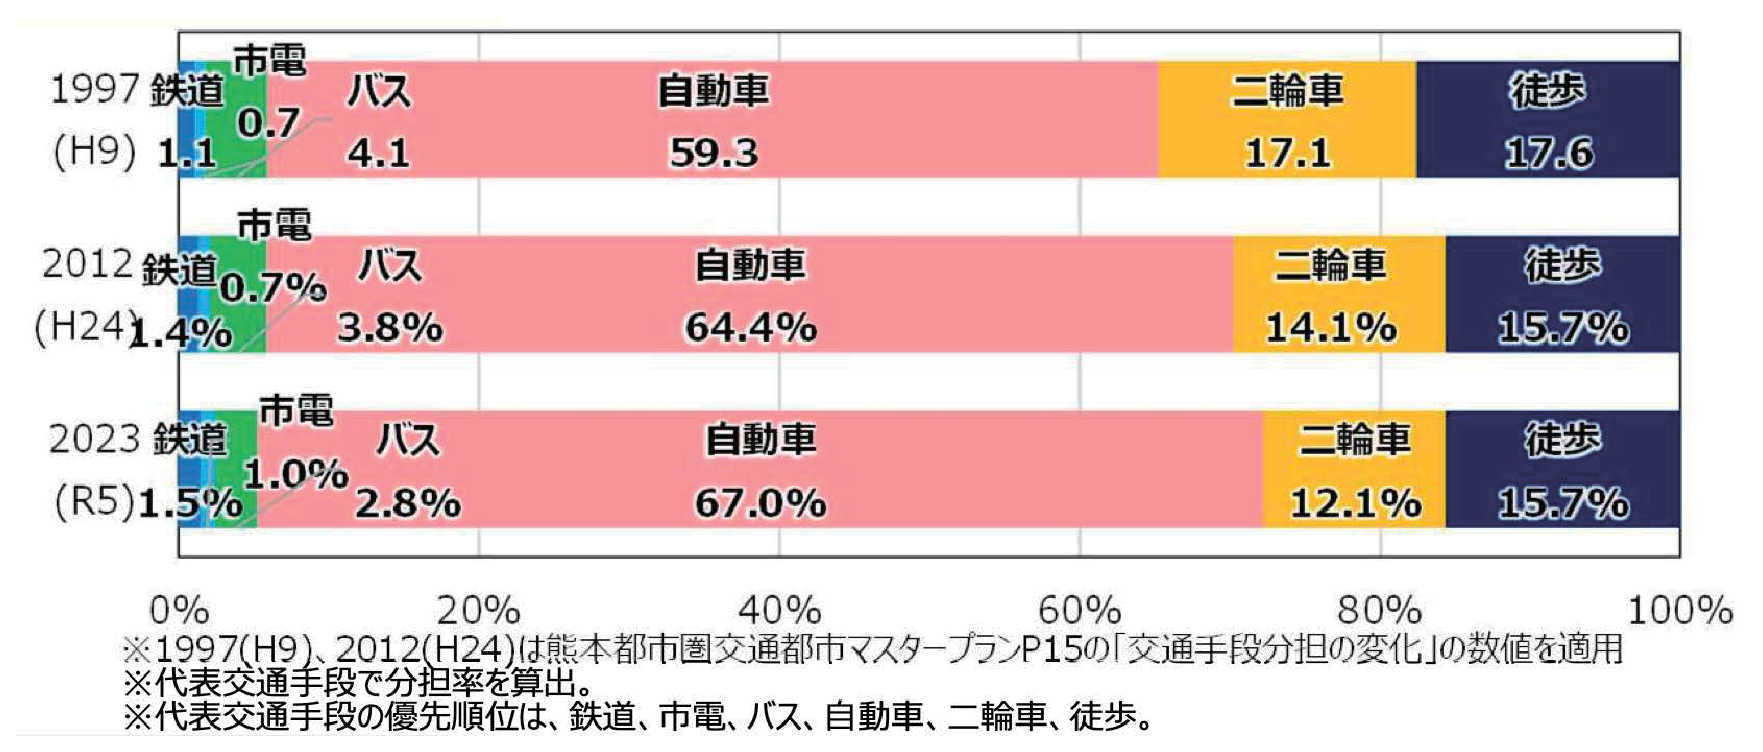
\includegraphics[width=0.8\textwidth]{picture/mode_kumamoto.eps}
    \caption{2023年熊本都市圏パーソントリップ調査の交通手段分担率\cite{kumamoto}}
    \label{fig:mode_kumamoto}
\end{figure}

\begin{figure}[htbp]
    \centering
    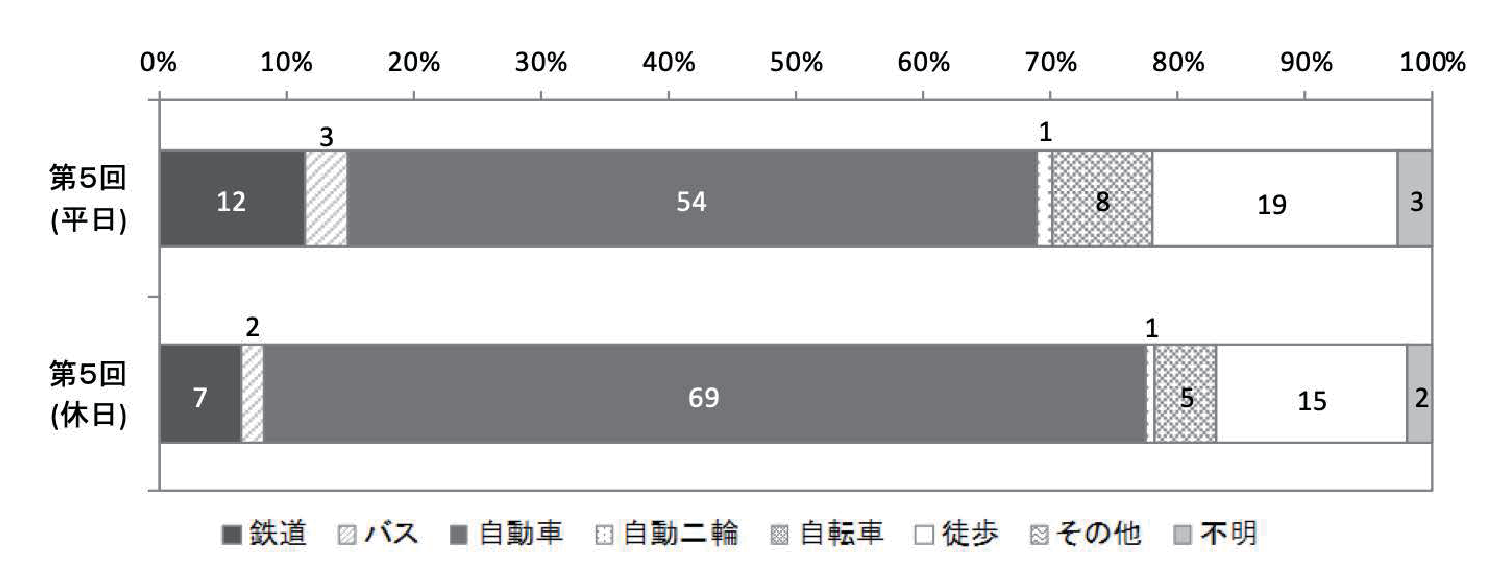
\includegraphics[width=0.8\textwidth]{picture/mode_sendai.eps}
    \caption{2017年仙台都市圏パーソントリップ調査の交通手段分担率\cite{sendai}}
    \label{fig:mode_sendai}
\end{figure}


\color{red}
\begin{framed}
\noindent
\textbf{\large 松山都市圏は車社会である。特に近年、自転車と徒歩による移動が減少し、自動車の利用が増加している。}
\end{framed}
\color{black}


\clearpage
\subsection{年齢別の交通手段分担率}
年齢別の交通手段分担率を図\ref{fig:mode_share_age}に示す。
自動車利用率は、若年層で低く、30〜50歳代をピークとして上昇し、その後減少する傾向にある。
18歳以下の年代は、運転免許を保持していないため、自動車の分担率が41\%と低い。
その分、徒歩の分担率が34\%と高い割合を占める。
19〜22歳の大学生の年代は、自動車分担率が35\%と全世代で最小である。
一方で、自転車の分担率が26\%、原付・二輪の分担率が18\%と、全世代で最大であり、小型のモビリティを盛んに利用している。
また、鉄道の分担率も7\%と全世代で最大であり、自動車に依存しない生活を送っていると言える。

その後、年齢が上がるにつれて、徒歩・自転車・原付・二輪・鉄道の分担率が減少し、自動車の分担率が上昇する。
自動車利用は、30〜50歳代にピークを迎え、その後は減少に転じる。
減少した分は、主に徒歩の分担率が増加し、公共交通の分担率は増加しないことに特徴がある。
また、60歳代以降は、他の人の運転する自動車への同乗が増加し、60~80歳代で15~16\%、90歳代で36\%を占める。

\begin{figure}[htbp]
    \centering
    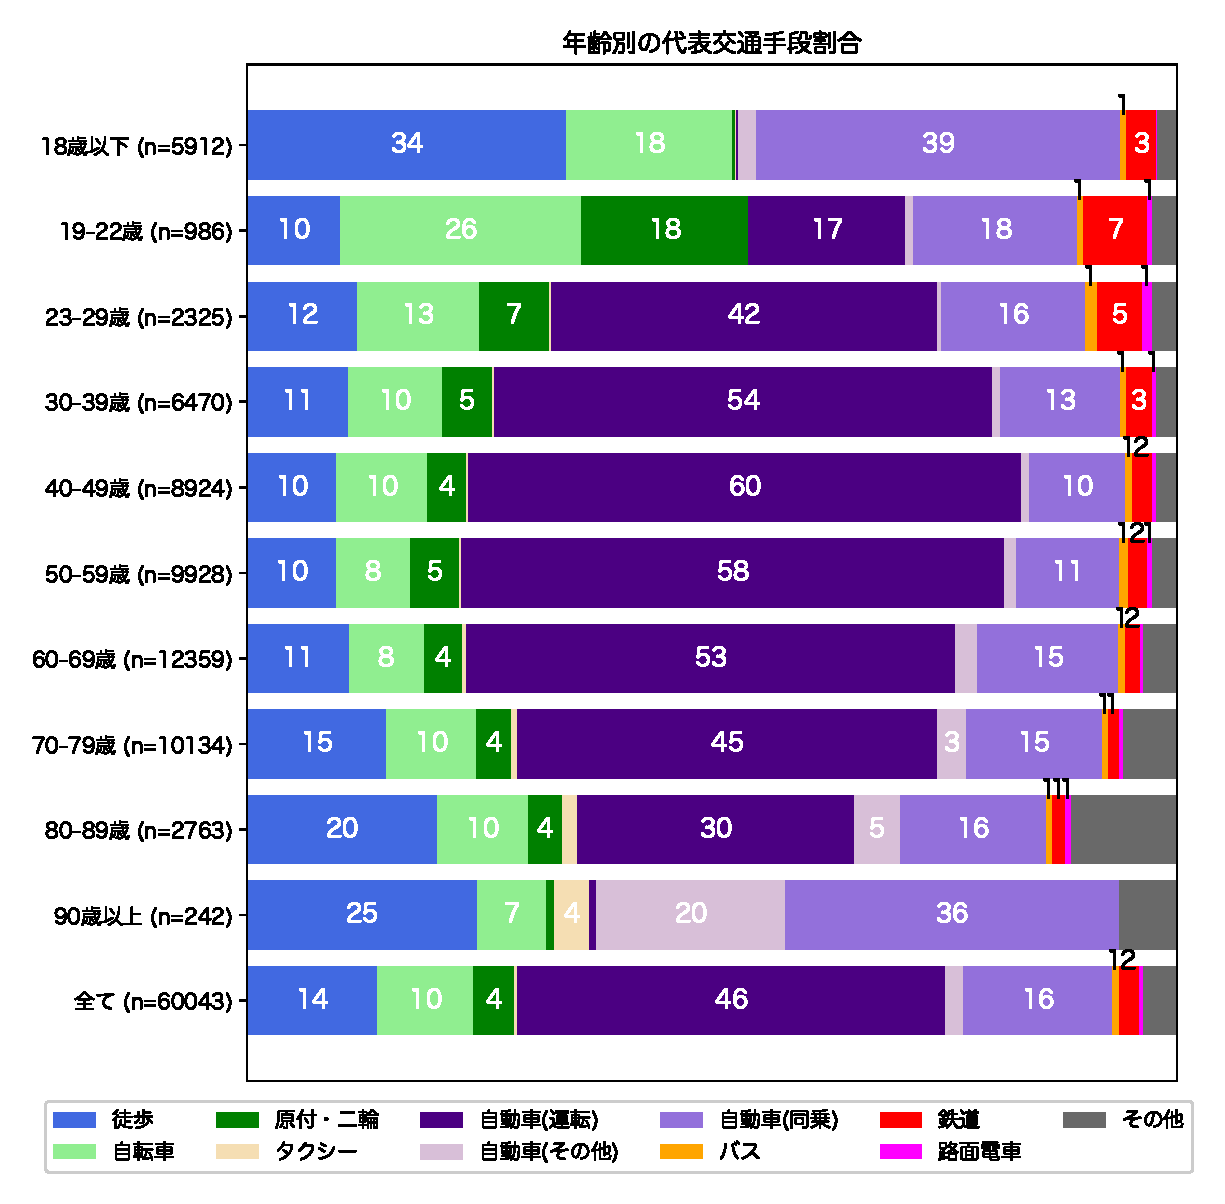
\includegraphics[width=1.0\textwidth]{picture/mode_share_age.eps}
    \caption{年齢別の交通手段分担率}
    \label{fig:mode_share_age}
\end{figure}

\clearpage
性・年齢別の代表交通手段分担率 (図\ref{fig:mode_share_gender_age})によると、性別によって交通手段利用に顕著な差は存在しない。

\begin{figure}[htbp]
  \centering
	\subfigure[男性]{%
		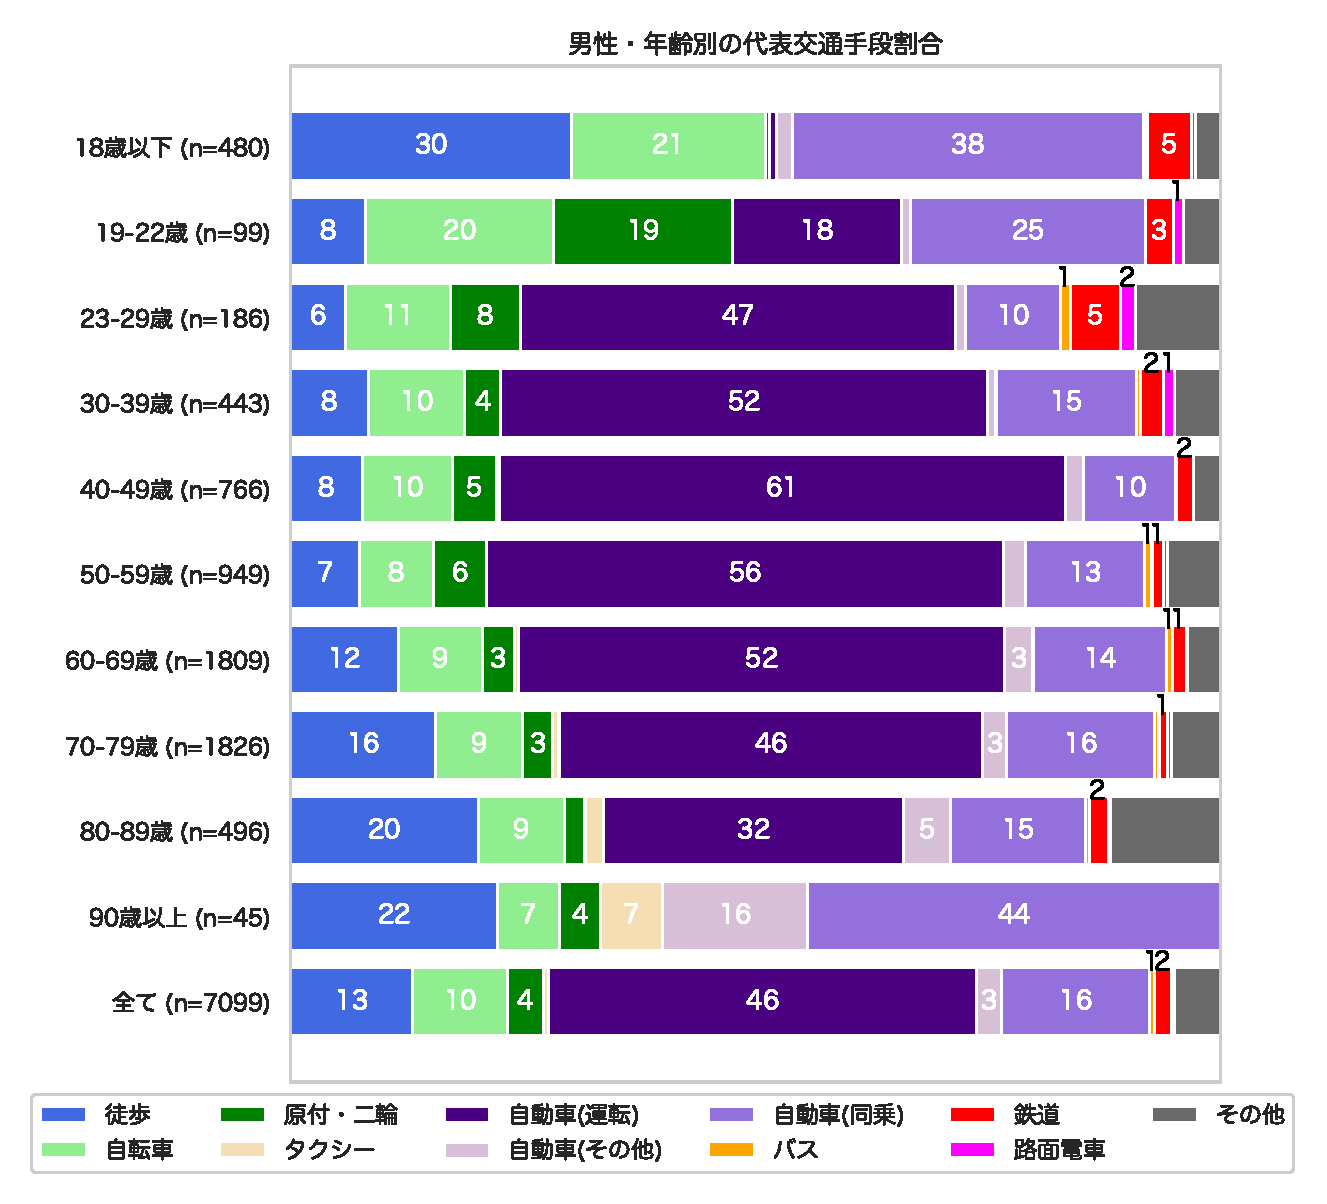
\includegraphics[clip, width=0.5\columnwidth]{picture/mode_share_male_age.eps}}%
	\subfigure[女性]{%
		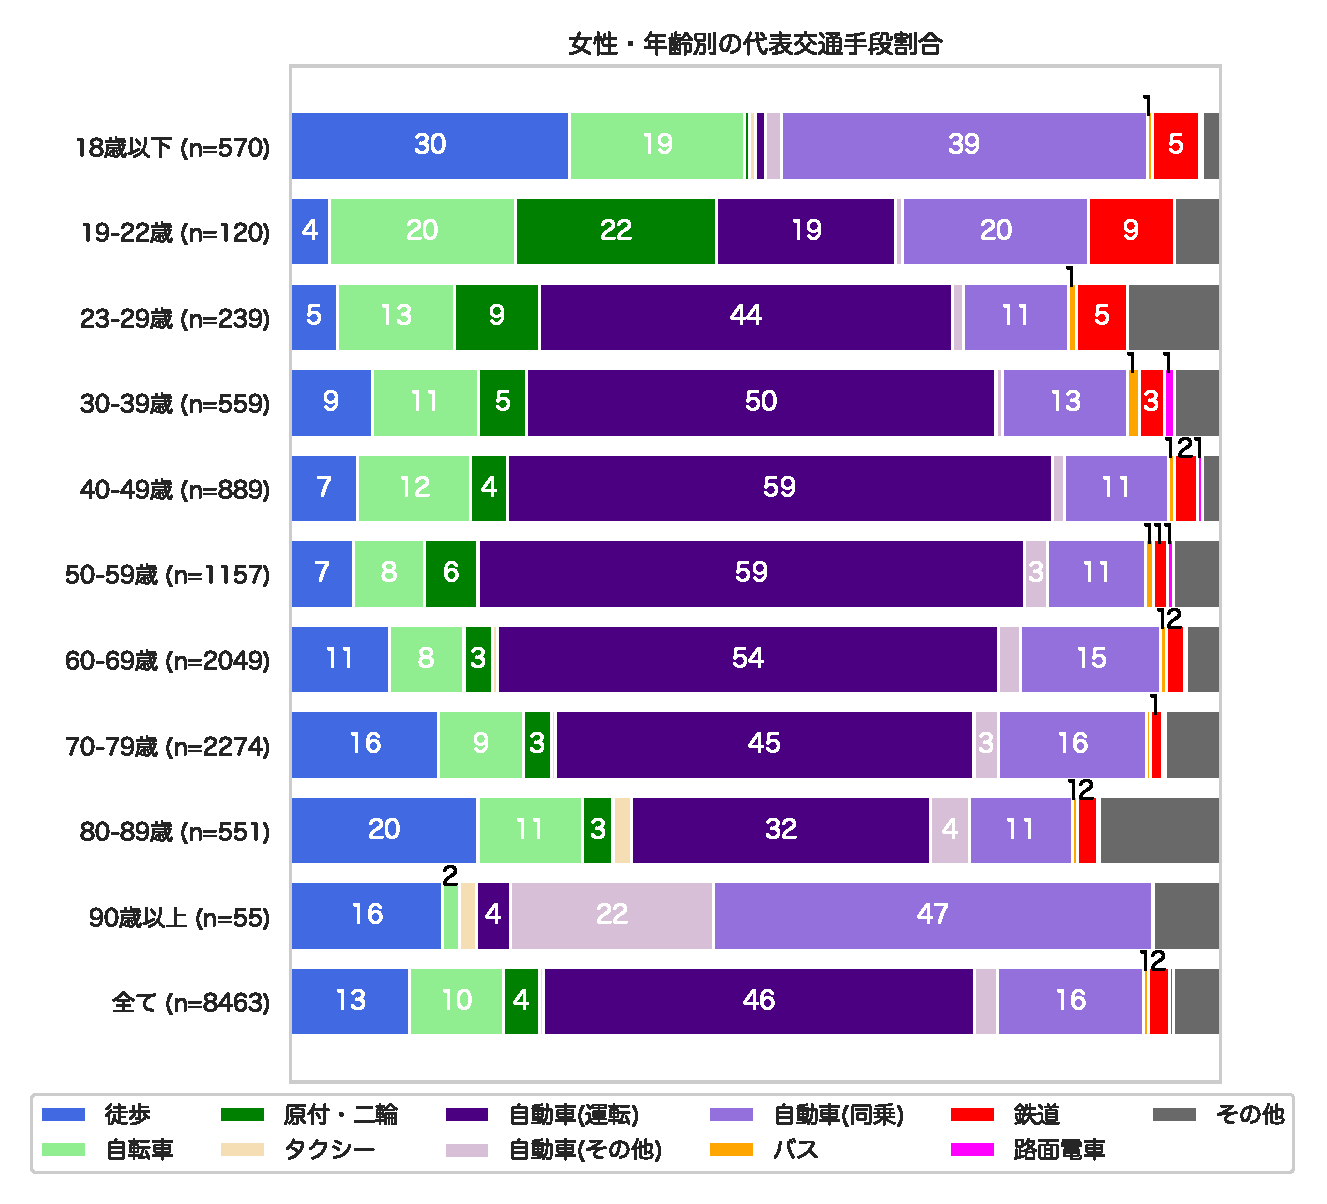
\includegraphics[clip, width=0.5\columnwidth]{picture/mode_share_female_age.eps}}%
	\caption{性・年齢別の代表交通手段割合}
	\label{fig:mode_share_gender_age}
\end{figure}

\color{red}
\begin{framed}
\noindent
\textbf{\large 20歳代までの若年層は、徒歩・自転車・原付の利用割合が高く、公共交通の利用も比較的多い。しかし、年齢が上がるにつれて自動車の利用が増加し、30〜60歳代で移動の約7割を占める。}
\end{framed}
\color{black}



\clearpage
\subsection{年齢・目的別の交通手段分担率}
目的・年齢別の交通手段分担率を、図\ref{fig:mode_share_commute}, \ref{fig:mode_share_shopping}, \ref{fig:mode_share_leisure}, \ref{fig:mode_share_tour}, \ref{fig:mode_share_hospital}に示す。

通勤・通学の交通手段 (図\ref{fig:mode_share_commute})は、若年層では、徒歩・自転車・原付・二輪が多く、19〜22歳では64\%、23〜29歳では39\%を占める。
特に、他の目的と比較して、自転車の分担率が高いことが特徴である。
また、通勤・通学は他の目的と比較して、鉄道やバスの分担率が高く、1割程度を占める。
これは、郊外の住宅地から松山市中心部の職場や学校への鉄道需要が存在するためと考えられる。
しかし、年齢が上がるにつれて自動車の割合が増加し、30歳代以降はおよそ6割が自動車で通勤する。
%
\begin{figure}[htbp]
    \centering
    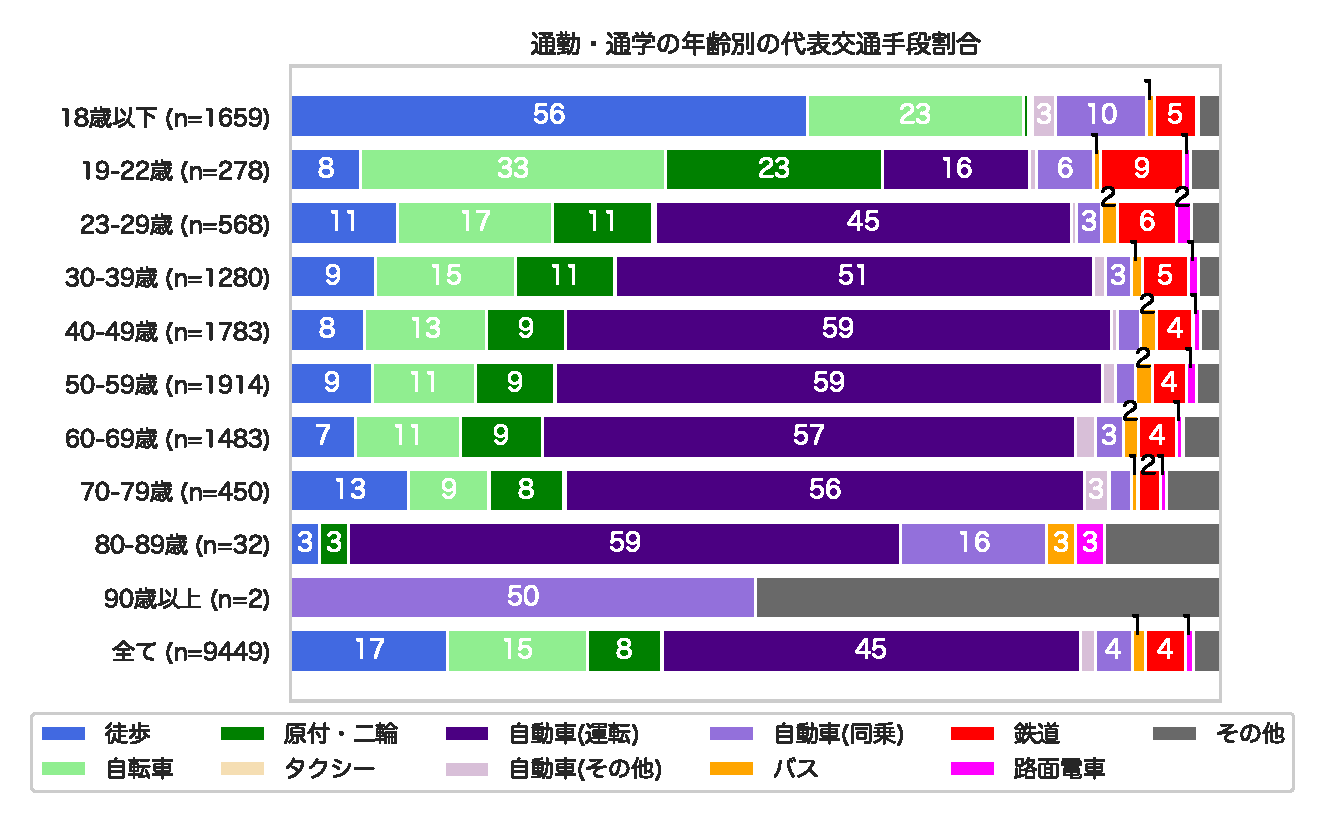
\includegraphics[width=1.0\textwidth]{picture/mode_share_通勤通学_age.eps}
    \caption{通勤・通学目的の年齢別交通手段分担率}
    \label{fig:mode_share_commute}
\end{figure}

買い物の交通手段 (図\ref{fig:mode_share_shopping})は、自動車の分担率が高く、20歳代で6割、30〜60歳代でおよそ75\%を占める。
これは、自宅近くでの買い物に加えて、郊外型のロードサイド店舗やショッピングモールを目的地とした買い物移動が多いためと考えられる。
一方で、若年層と高齢者では、徒歩と自転車の割合が、他の年代と比較して高い。
公共交通の利用は全年代を通してほとんど見られない。
%
\begin{figure}[htbp]
    \centering
    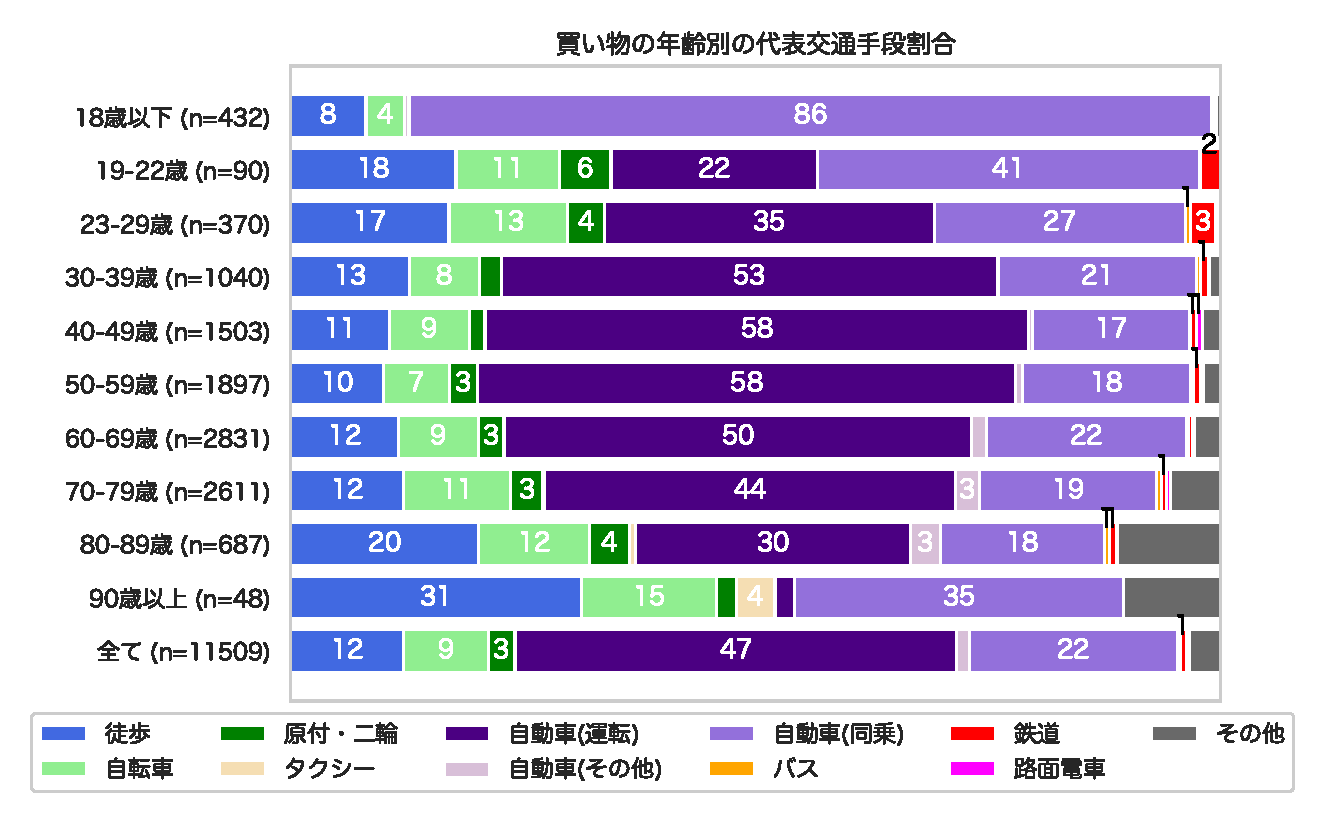
\includegraphics[width=1.0\textwidth]{picture/mode_share_買い物_age.eps}
    \caption{買い物目的の年齢別交通手段分担率}
    \label{fig:mode_share_shopping}
\end{figure}

食事・社交・娯楽の交通手段 (図\ref{fig:mode_share_leisure})も、買い物と同様に、自動車中心で、若年層では徒歩・自転車・原付の利用が見られる。
%
\begin{figure}[htbp]
    \centering
    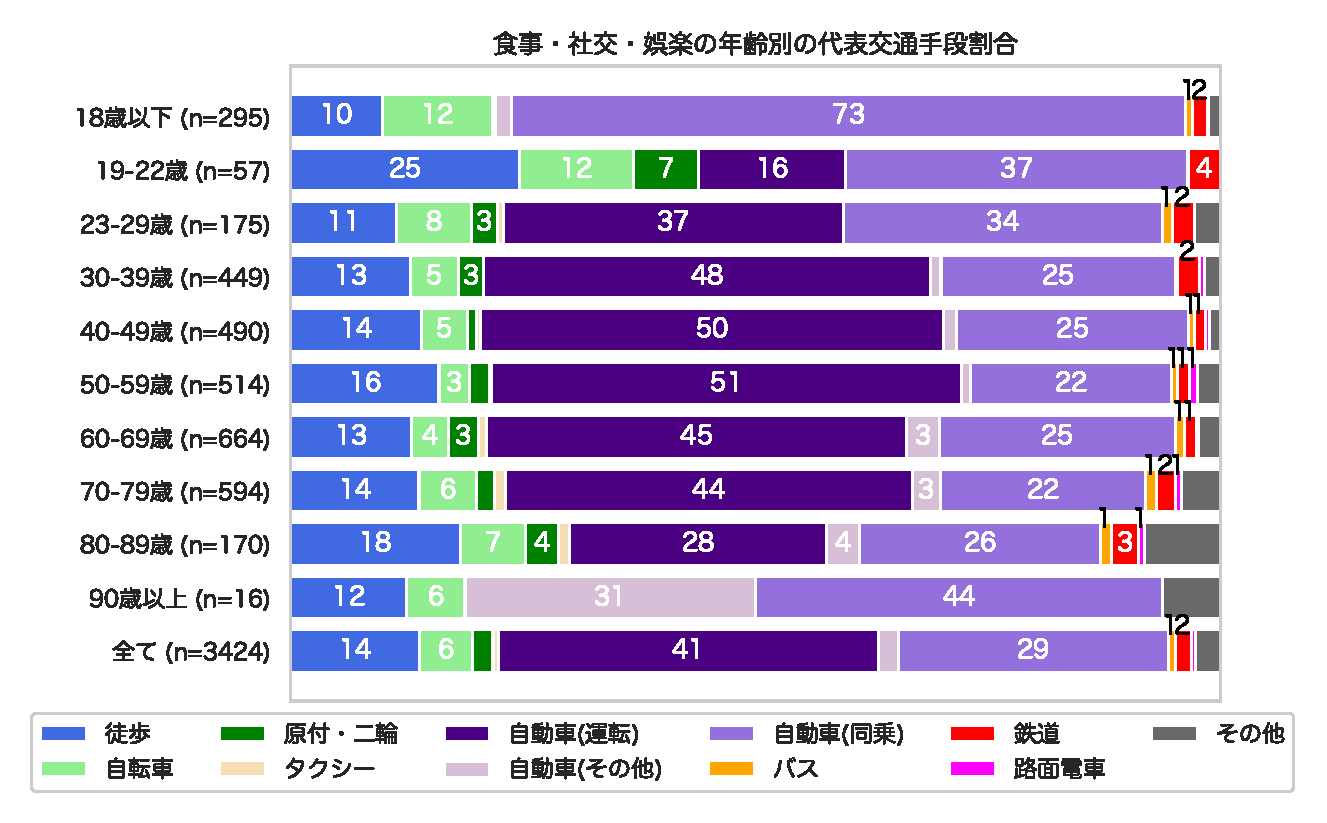
\includegraphics[width=1.0\textwidth]{picture/mode_share_食事・社交・娯楽_age.eps}
    \caption{食事・社交・娯楽目的の年齢別交通手段分担率}
    \label{fig:mode_share_leisure}
\end{figure}

観光・行楽・レジャーの交通手段 (図\ref{fig:mode_share_tour})は、他の目的と比較して鉄道の利用が若干多い。
また、60歳以上の高齢層において徒歩の割合が他の目的と比較して高いことも特徴である。
自動車の分担率は、若年層で6割程度、30〜50歳代で7割程度と高い水準である。
%
\begin{figure}[htbp]
    \centering
    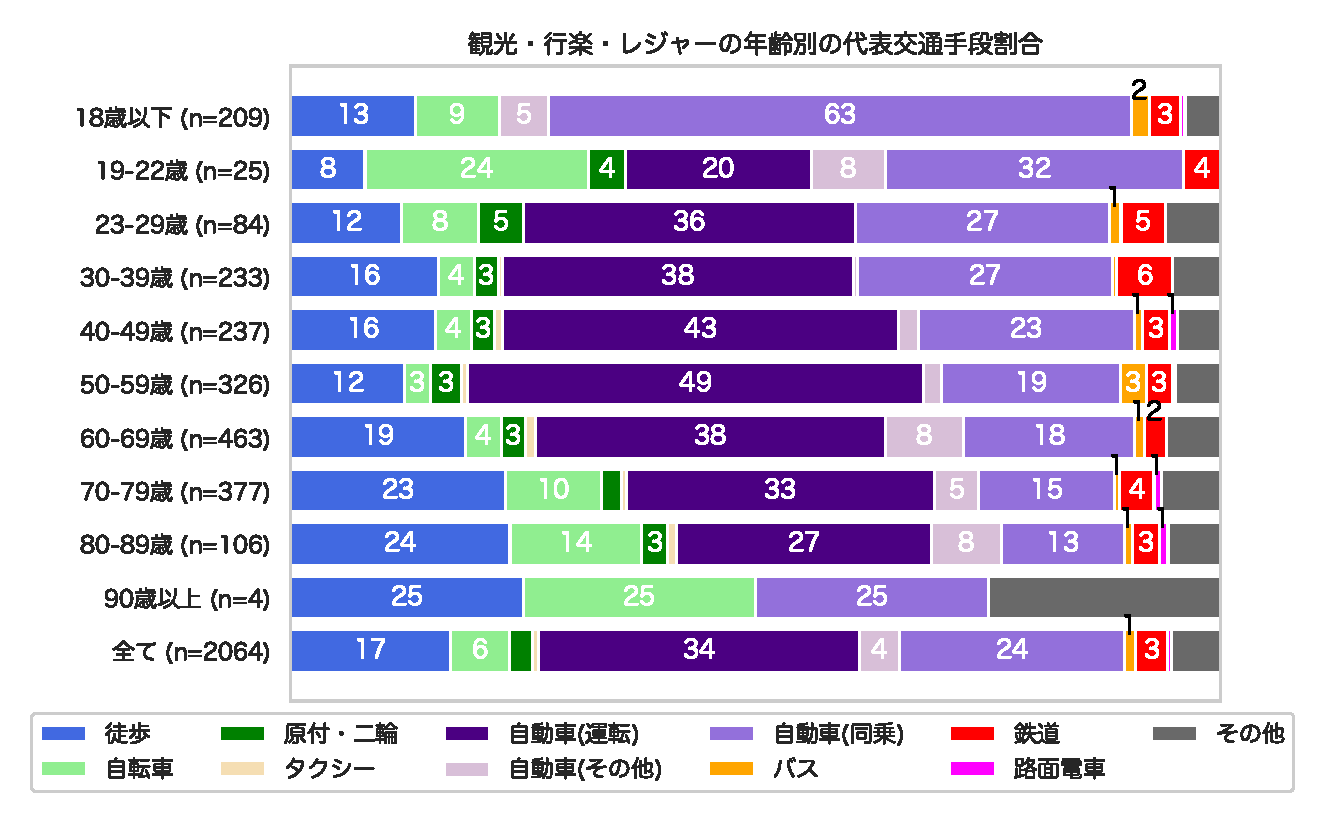
\includegraphics[width=1.0\textwidth]{picture/mode_share_観光・行楽・レジャー_age.eps}
    \caption{観光・行楽・レジャー目的の年齢別交通手段分担率}
    \label{fig:mode_share_tour}
\end{figure}

通院の交通手段 (図\ref{fig:mode_share_hospital})は、高齢者を中心にタクシーやその他のモビリティの割合が高い。
通院の際は、自宅からdoor-to-doorの移動の需要があるため、デマンド型の交通の需要が高いと考えられる。
%
\begin{figure}[htbp]
    \centering
    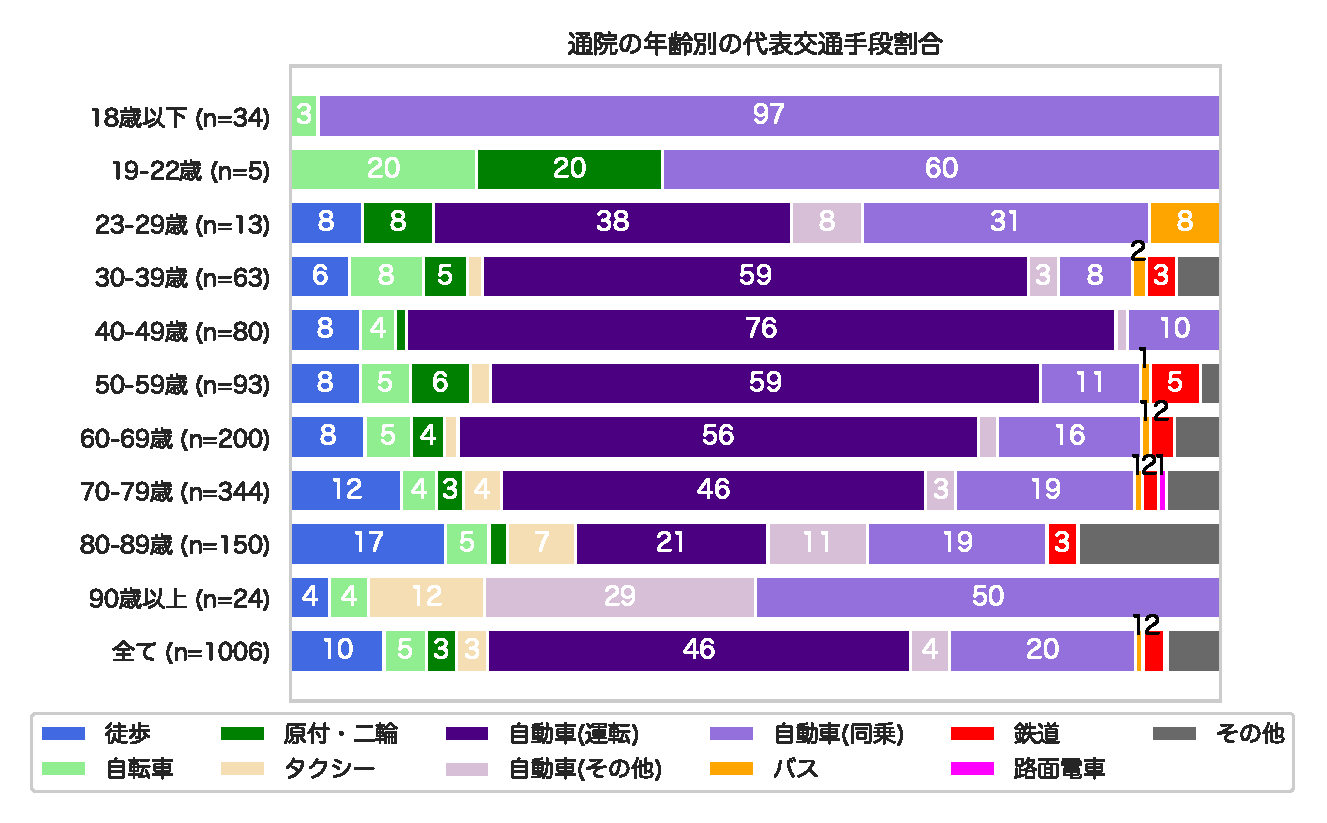
\includegraphics[width=1.0\textwidth]{picture/mode_share_通院_age.eps}
    \caption{通院目的の年齢別交通手段分担率}
    \label{fig:mode_share_hospital}
\end{figure}

\clearpage
\color{red}
\begin{framed}
\noindent
\textbf{\large 通勤・通学の移動は、若年層を中心に徒歩・二輪・公共交通の分担率が比較的高いが、買い物や食事・社交・娯楽の移動は6割から8割を自動車の移動が占め、公共交通はほとんど使われない。高齢者の通院や買い物の移動にタクシーが使われており、door-to-doorのデマンド型の交通の需要が存在する。}
\end{framed}
\color{black}



\clearpage
\subsection{距離帯別の交通手段分担率}

距離帯・年齢別の交通手段分担率を図\ref{fig:mode_share_dist}に示す。
200m未満の移動でも、23〜69歳の年代では、3割から4割程度の移動が自動車で行われている。
500mまでの移動では、徒歩と自転車による移動が全体の半分以上を占めるが、500m以上では自動車の割合が卓越し、500m-1kmでは50\%、1km-2kmでは62\%、2km-5kmでは73-74\%、5km以上では約8割を占める。
一方、若年層は徒歩と自転車で移動する距離が他の年代より顕著に長い。
200m-500mの移動について、29歳以下は70〜88\%が徒歩と自転車で移動し、他の年代より20〜30\%ほど多い。
500m〜1kmの距離帯でも、18歳以下は74\%、19〜22歳は56\%、23〜29歳は59\%が徒歩と自転車で移動する。
一方で、30歳代以上では、500m〜1kmの距離帯について、5割から6割の移動が自動車で行われる。

若年層の中距離の移動には、原付・二輪が多く使われることも特徴である。
特に、19〜22歳の大学生の年代では、1km〜10kmの移動の2割から3割が原付・二輪であり、自転車と並んで若年層の中距離移動の重要な交通手段となっている。

3km以上の移動には、20歳代を中心に鉄道の利用が増加する。
特に、19〜22歳の3km〜5kmの移動や、29歳以下の5km〜10kmの移動の1割が鉄道によるものである。
路面電車は、23〜29歳の1km〜2kmの移動で5\%を占め、1km〜3kmの距離帯の移動に比較的よく使われる。
これらのことから、20歳代以下の徒歩・自転車・公共交通を組み合わせた移動を、今後も継続してもらう政策的取り組みや、30歳代以上の年代にも広げていくことが、公共交通中心のまちづくりのために必要であると言える。


\begin{figure}[htbp]
    \centering
    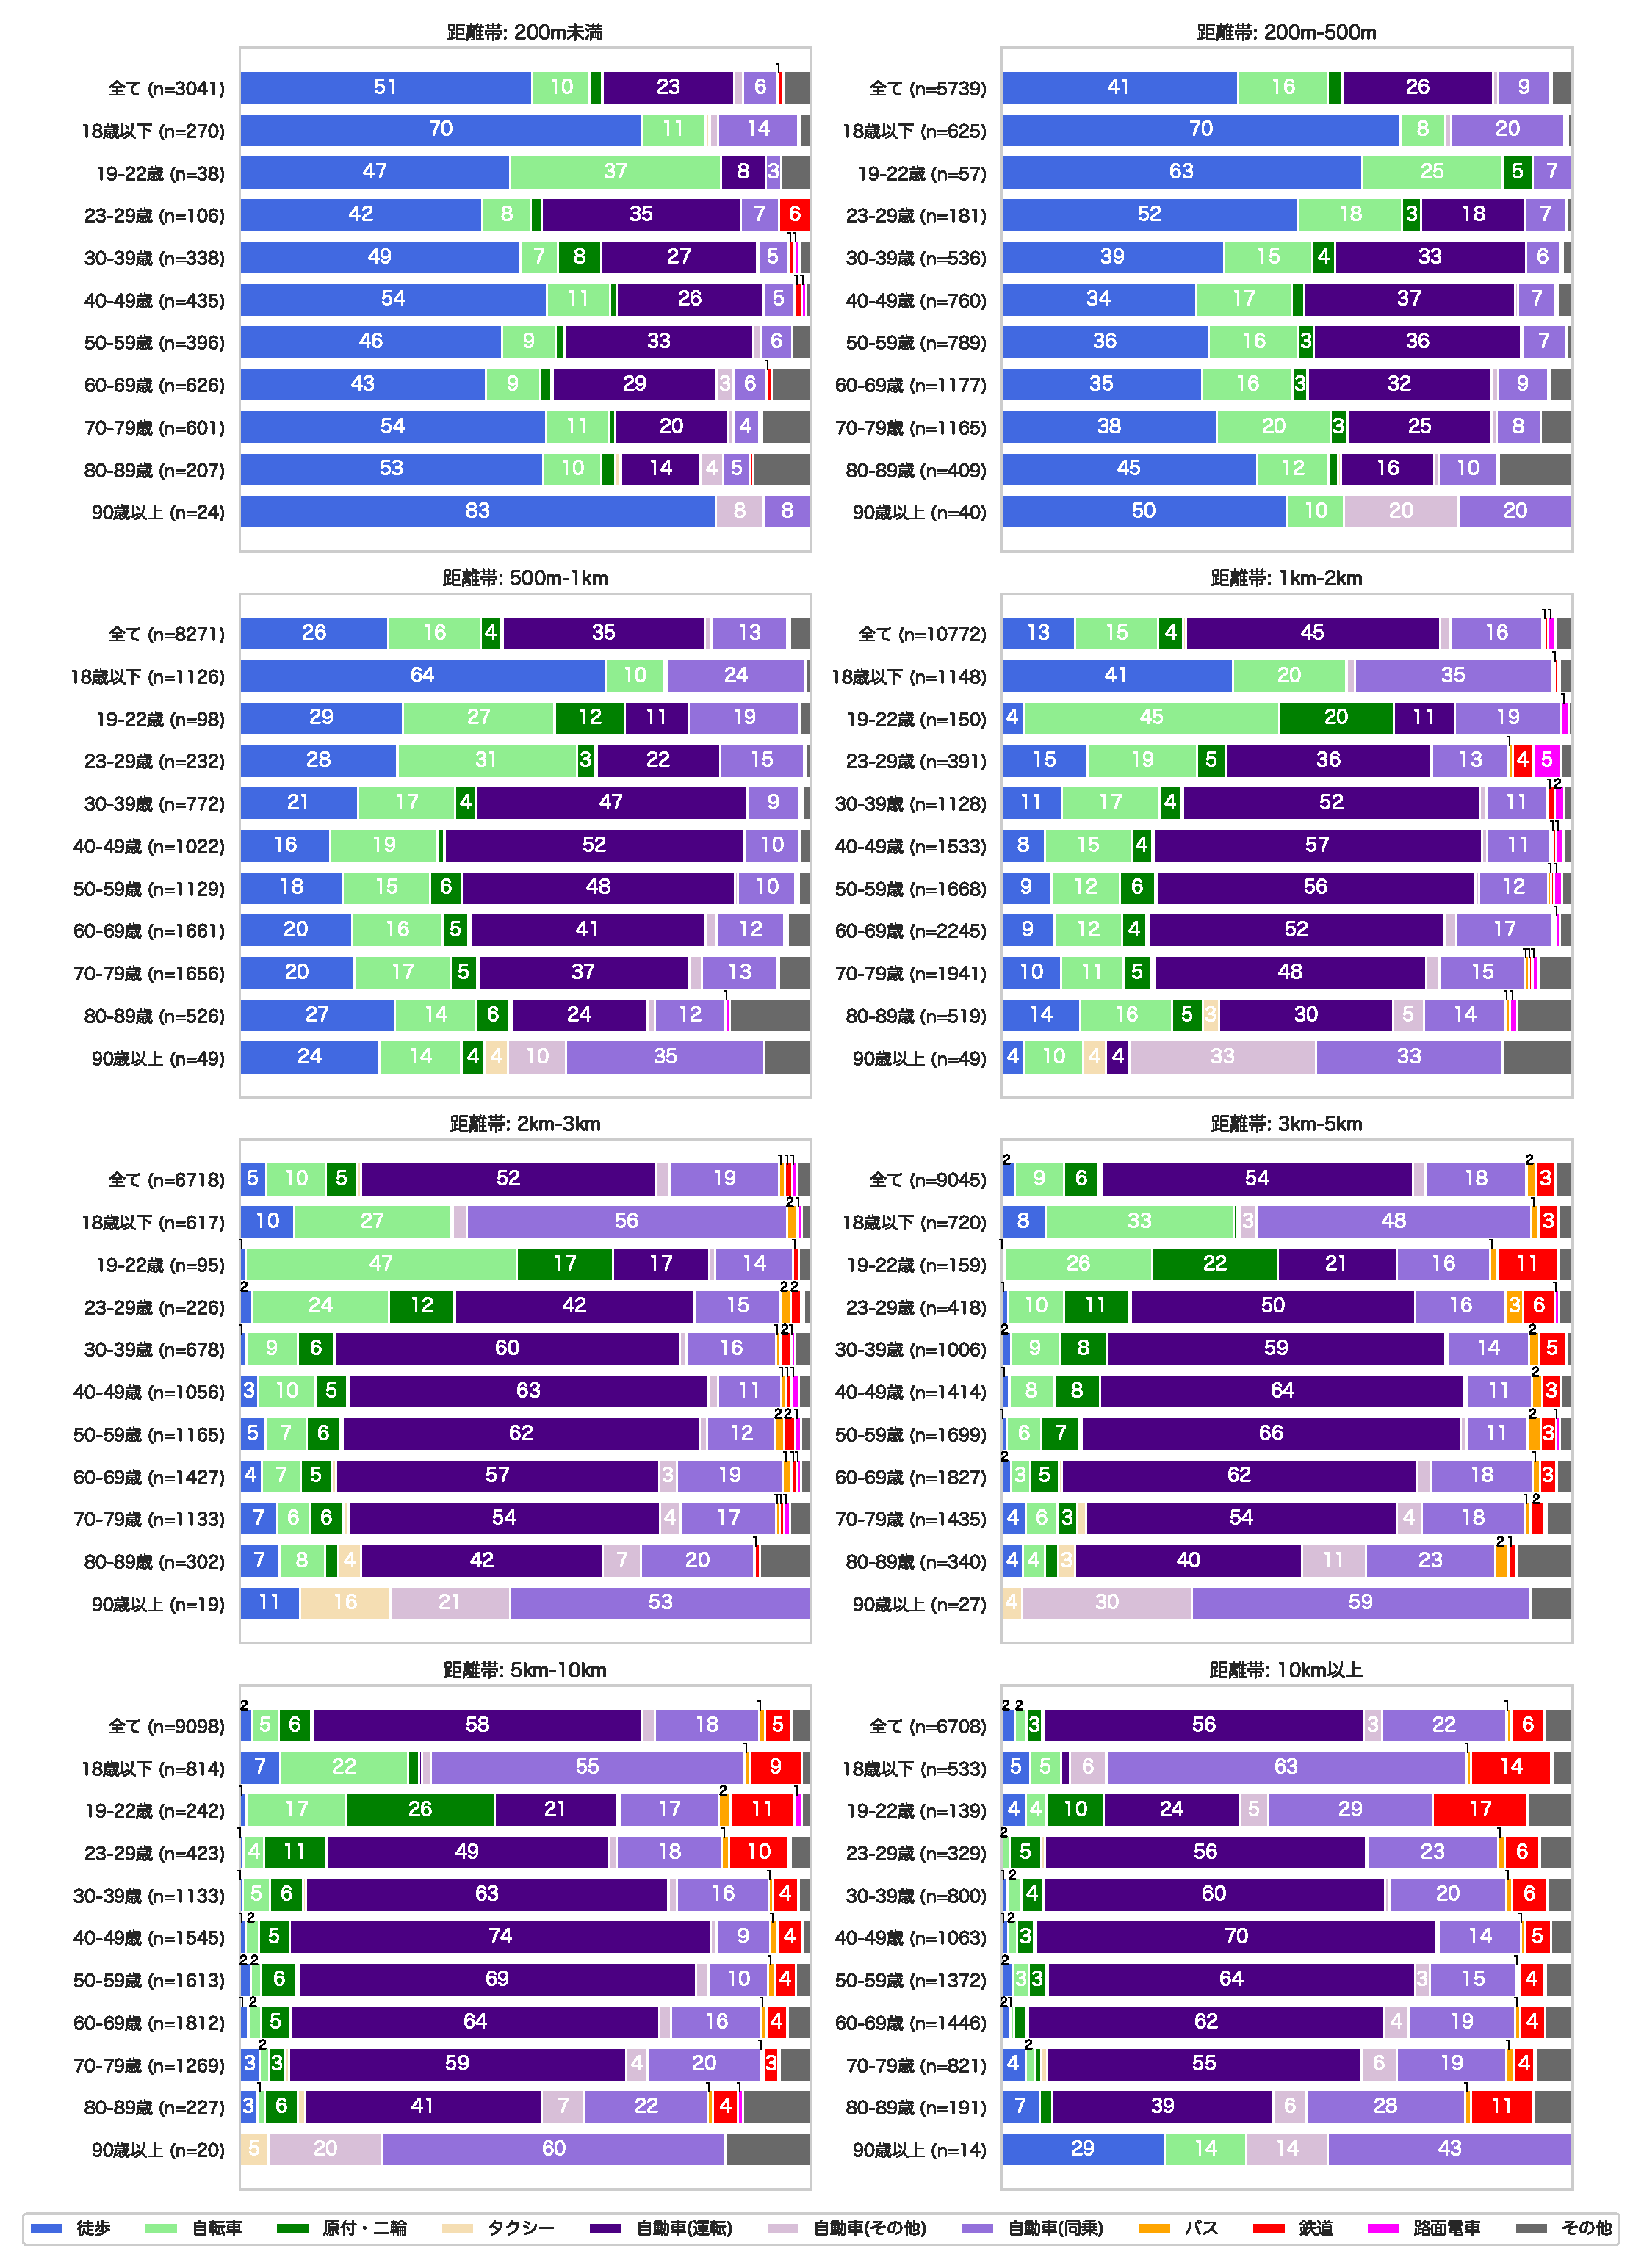
\includegraphics[width=1.0\textwidth]{picture/mode_share_age_dist.eps}
    \caption{距離帯・年齢別の交通手段分担率}
    \label{fig:mode_share_dist}
\end{figure}

\color{red}
\begin{framed}
\noindent
\textbf{\large 23〜69歳の年代は、200m未満の移動でも3〜4割の移動が自動車で行われ、500m以上の移動は6〜9割が自動車である。一方、19〜22歳の大学生年代の交通手段選択は特異的で、近距離は徒歩・自転車、中距離は自転車・原付、長距離は鉄道の利用が、それ以降の年代と比較して卓越している。}
\end{framed}
\color{black}


\clearpage
\subsection{地区間の移動の交通手段分担率}
次に、各地区を出発するトリップの代表交通手段分担率を分析することにより、地域ごとの交通手段の特徴を明らかにする。
各図内の棒グラフは、目的地ごとの代表交通手段割合を表し、トリップ数の多い順に上から並んでいる。

なお、松山市23区 (JR松山駅)、松山市24区 (三津埠頭)、松山市25区 (松山観光港)、松山市26区 (中央卸売市場)、松山市28区 (中島)、伊予市2区 (伊予南部山地)、伊予市3区 (伊予西部山地)、東温市2区 (東温市東部山地)、砥部町2区 (砥部南部山地)はデータ数が少なかったため分析から除いた。

\subsubsection{松山市1区 (市駅、大街道、松山城)}
松山市中心部は、徒歩と自転車の分担率が高く、松山市1区の地区内移動は、8割超を徒歩と自転車が占め、ウォーカブルなまちが形成されている。
また、松山市1区から松山市3区 (愛媛大、松山東高校、祝谷)、松山市1区から松山市6区 (衣山、宮田町)のトリップは、路面電車と鉄道が約1割を占めており、松山市駅エリアを中心に、中心市街地内の移動に路面電車と鉄道が利用されている。
一方で、松山市1区と松山市5区 (土橋、空港通り、南江戸)の間のトリップは、自動車が6割を占めており、中心部と周縁部との間では、自動車の利用が多い。

理想的には、トリップ数の多い同一地区内の移動は徒歩・自転車、次にトリップ数の多い中距離の移動は公共交通、公共交通では不便な地区や需要の少ない地域間の移動は自動車を利用することが望ましいと考えられる。
つまり、各グラフの上部の需要の多い移動は徒歩と自転車中心、中部はそれに加えて公共交通利用、下部の需要の少ない移動は自動車で補完する交通手段の構成が望ましいと言える。
松山市中心部は概ねその構成を満たしている。
%
\begin{figure}[H]
    \centering
    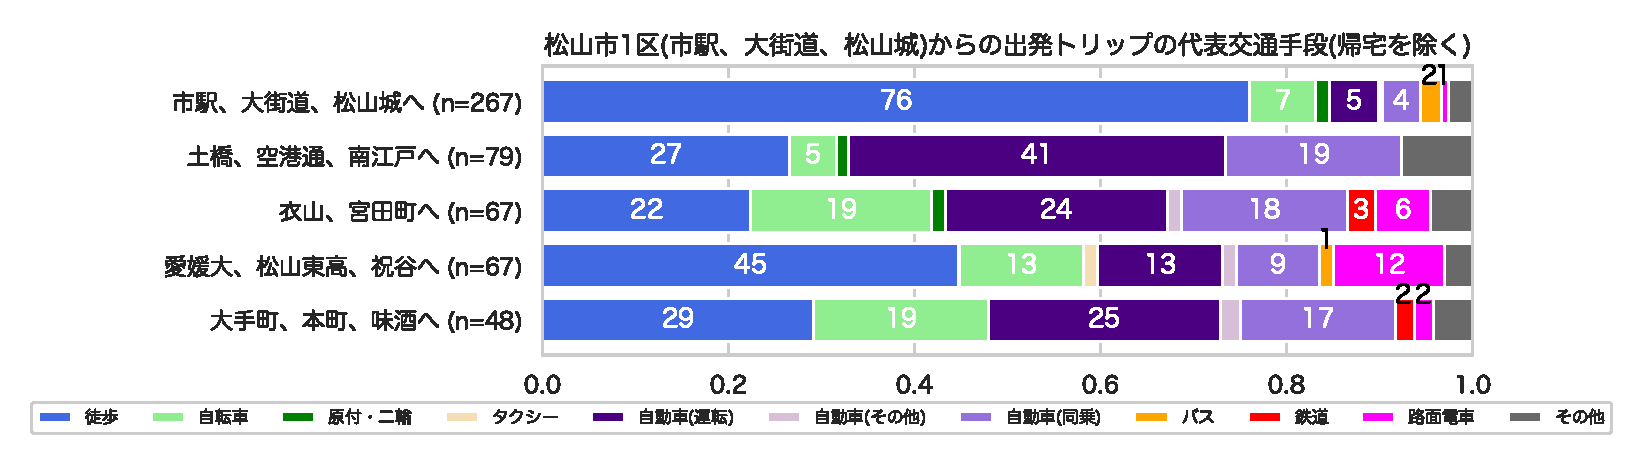
\includegraphics[width=1.0\textwidth]{picture/mode_share_松山市1区.eps}
    \caption{松山市1区を出発するトリップの交通手段割合}
    \label{fig:mode_share_1}
\end{figure}

\subsubsection{松山市2区 (大手町、本町、味酒)}
松山市2区も1区と同様に、地区内移動に占める徒歩と自転車の割合が高く、74\%を占める。
松山市2区から松山市1区 (市駅、大街道、松山城)間の移動は、路面電車と鉄道が9\%を占めており、公共交通の利用も多い。
一方で、松山市5区 (土橋、空港通り、南江戸)や松山市7区 (木屋町、山越、姫原)の周縁部への移動は、自動車の分担率が55〜63\%を占める。
%
\begin{figure}[H]
    \centering
    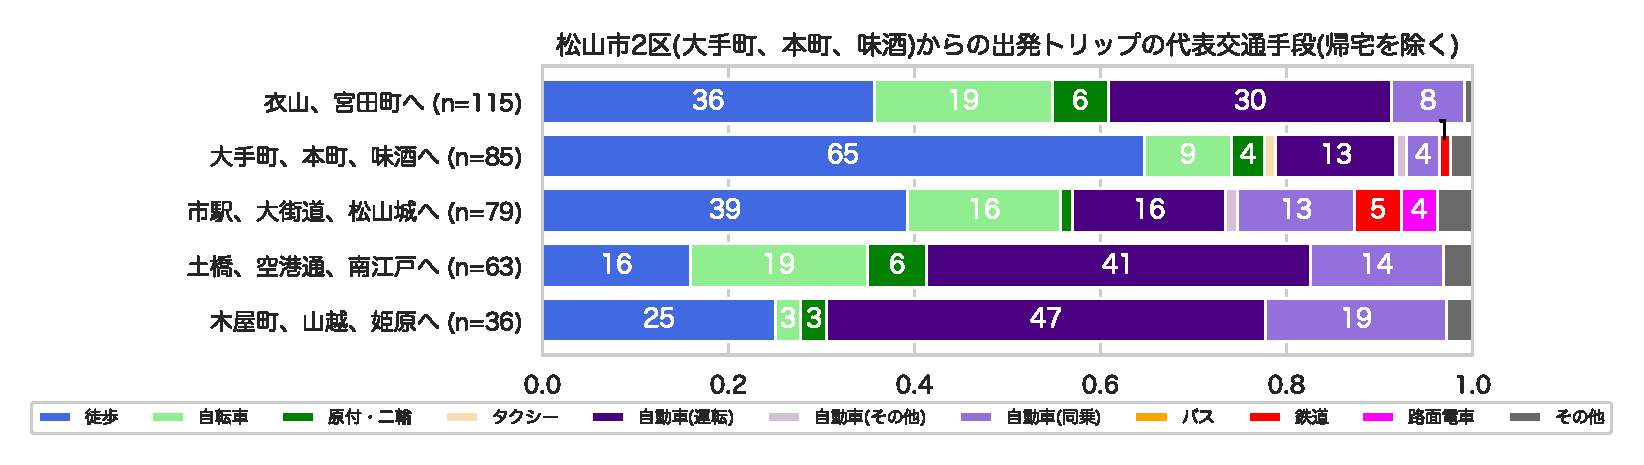
\includegraphics[width=1.0\textwidth]{picture/mode_share_松山市2区.eps}
    \caption{松山市2区を出発するトリップの交通手段割合}
    \label{fig:mode_share_2}
\end{figure}

\subsubsection{松山市3区 (愛媛大、松山東高校、祝谷)}
松山市3区から松山市1区 (市駅、大街道、松山城)への移動は、路面電車が11\%を占めており、特徴的な手段構成である。
また、地区内移動や、松山市1区 (市駅、大街道、松山城)、松山市22区 (道後温泉、石手寺)への移動は、徒歩と自転車の分担率が高く、6〜7割程度を占めており、徒歩・自転車・公共交通中心の移動が達成されている。
%
\begin{figure}[H]
    \centering
    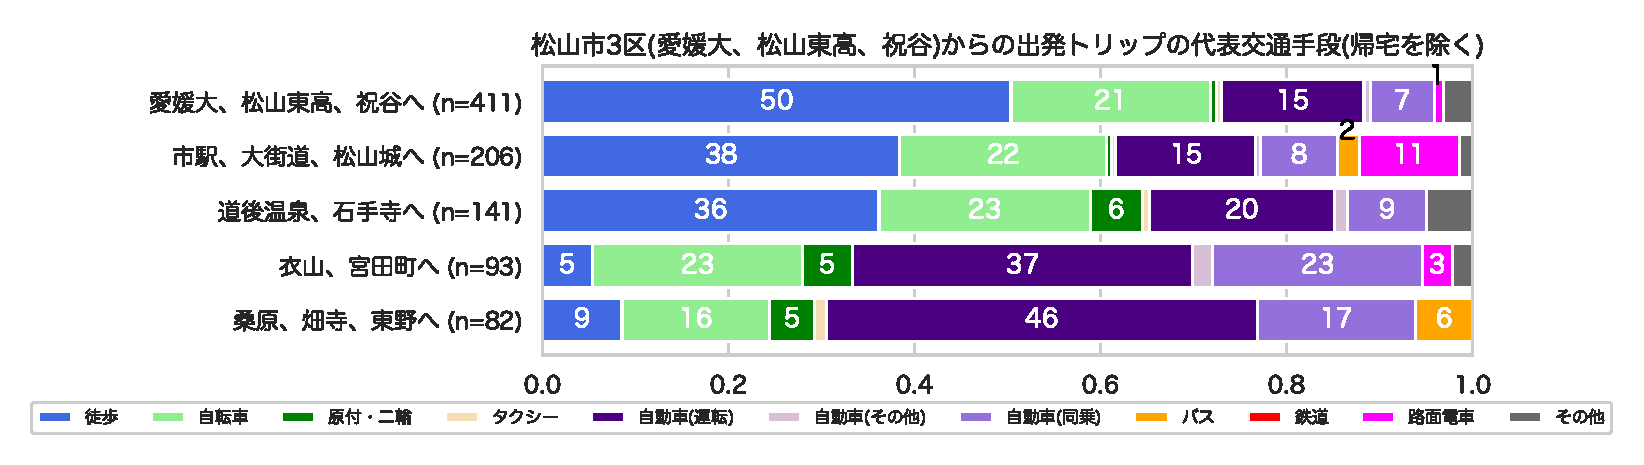
\includegraphics[width=1.0\textwidth]{picture/mode_share_松山市3区.eps}
    \caption{松山市3区を出発するトリップの交通手段割合}
    \label{fig:mode_share_3}
\end{figure}

\subsubsection{松山市4区 (いよ立花駅、朝生田)}
中心部と比較すると、地区内移動における徒歩の分担率が低下し、自動車の分担率が上昇している。
地区内の移動の徒歩・自転車の分担率が中心部と比較して20\%程度少なく、近距離の移動でも自動車中心のライフスタイルが根付いていると言える。
松山市13区 (和泉南、古川北、石井、朝生田)や松山市10区 (桑原、畑寺、東野)といった周辺地域への移動需要は多いが、公共交通による移動はほぼ見られず、周縁部どうしをつなぐバス路線の整備や利便性向上が必要である。
%
\begin{figure}[H]
    \centering
    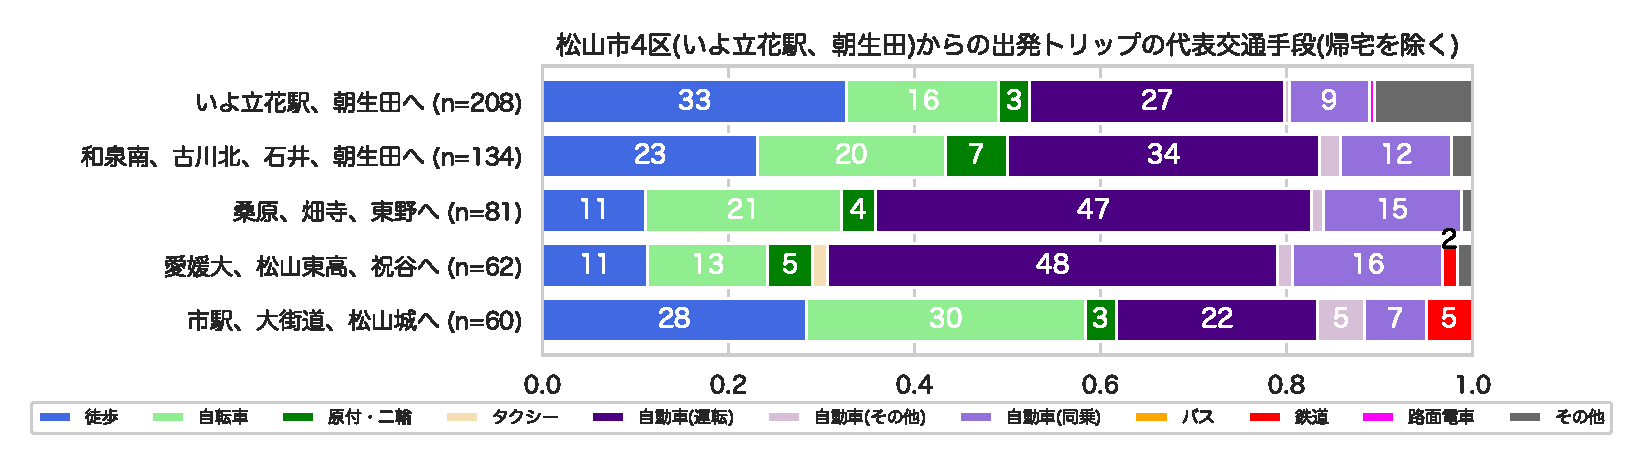
\includegraphics[width=1.0\textwidth]{picture/mode_share_松山市4区.eps}
    \caption{松山市4区を出発するトリップの交通手段割合}
    \label{fig:mode_share_4}
\end{figure}

\subsubsection{松山市5区 (土橋、空港通り、南江戸)}
松山市4区 (いよ立花駅、朝生田)と概ね同じ傾向で、地区内移動における自動車の分担率が高く、公共交通による移動がほとんど見られない。
特に、松山市15区 (垣生、余戸、土居田)や松山市6区 (衣山、宮田町)といった周辺地域への移動に占める自転車の割合が低いため、バイクシェアや自転車通行帯等のインフラ整備が必要と考えられる。
%
\begin{figure}[H]
    \centering
    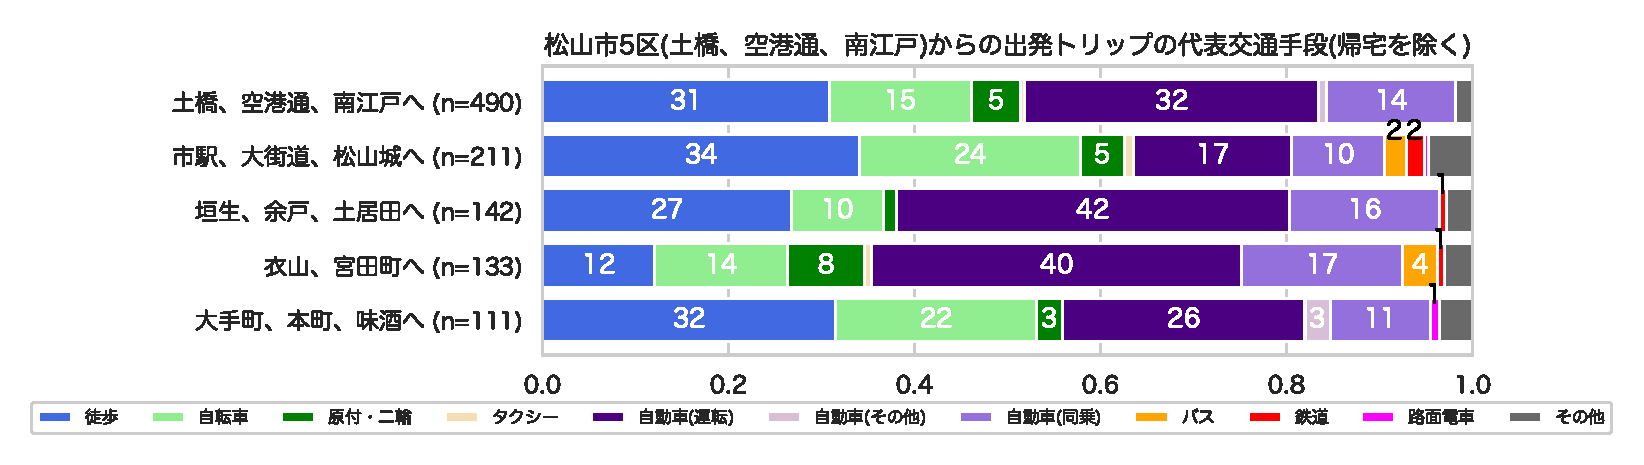
\includegraphics[width=1.0\textwidth]{picture/mode_share_松山市5区.eps}
    \caption{松山市5区を出発するトリップの交通手段割合}
    \label{fig:mode_share_5}
\end{figure}

\subsubsection{松山市6区 (衣山、宮田町)}
松山市1区 (市駅、大街道、松山城)への移動に、バスが3\%、鉄道が13\%、路面電車が9\%と高い割合を占めており、特徴的である。
地区内の移動は、徒歩と自転車が62\%を占めており、近い距離の移動に徒歩・自転車・公共交通中心の移動が達成されている。
一方で、松山市18区 (久万ノ台、谷町、北部山地)や松山市7区 (木屋町、山越、姫原)への移動は、需要が多い割に自動車の分担率が7〜8割を占めており、公共交通がほとんど使われていない。
このような郊外部へ向かう移動において、バスの利便性を高めたり、バイクシェア等の取り組みによって、自転車や公共交通の分担率を高めていく必要がある。
%
\begin{figure}[H]
    \centering
    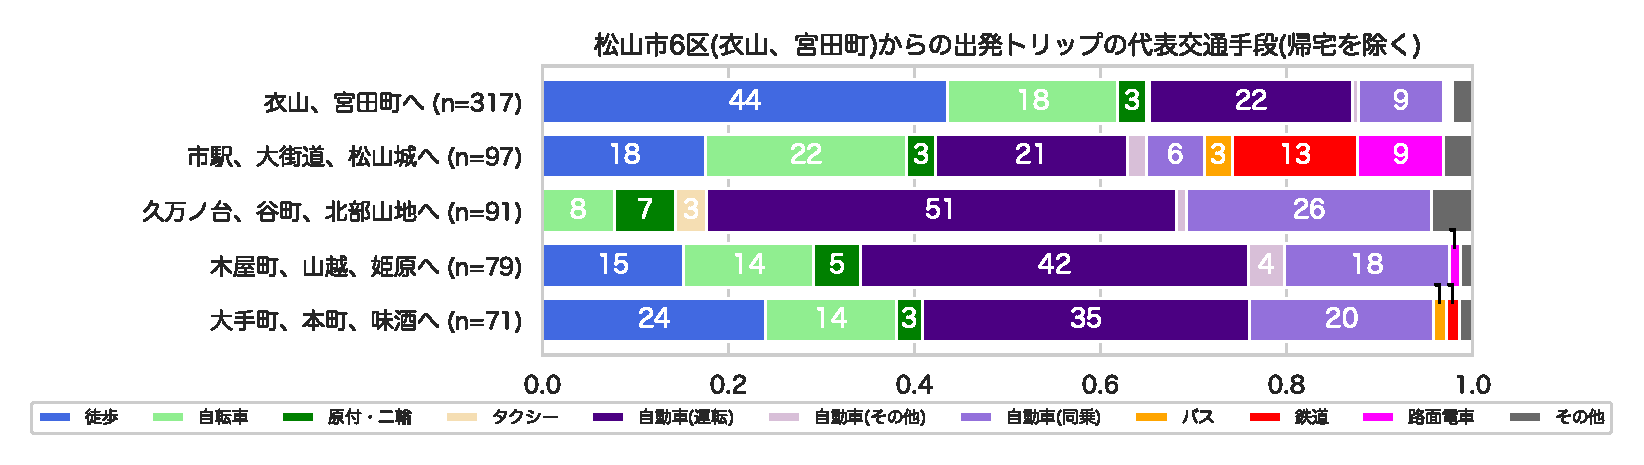
\includegraphics[width=1.0\textwidth]{picture/mode_share_松山市6区.eps}
    \caption{松山市6区を出発するトリップの交通手段割合}
    \label{fig:mode_share_6}
\end{figure}

\subsubsection{松山市7区 (木屋町、山越、姫原)}
松山市6区 (衣山、宮田町)への移動の5\%、松山市1区 (市駅、大街道、松山城)への移動の10\%を路面電車が占める。
松山市6区 (衣山、宮田町)と同様に、地区内の移動は、徒歩と自転車が60\%を占めており、近い距離の移動に徒歩・自転車・公共交通中心の移動が達成されている。
特に、松山市1区 (市駅、大街道、松山城)や松山市3区 (愛媛大、松山東高校、祝谷)への移動の約30\%が自転車によるもので、割合が大きい。
一方で、中心部と逆方向の松山市18区 (久万ノ台、谷町、北部山地)への移動は、自動車による移動が68\%を占める。
%
\begin{figure}[H]
    \centering
    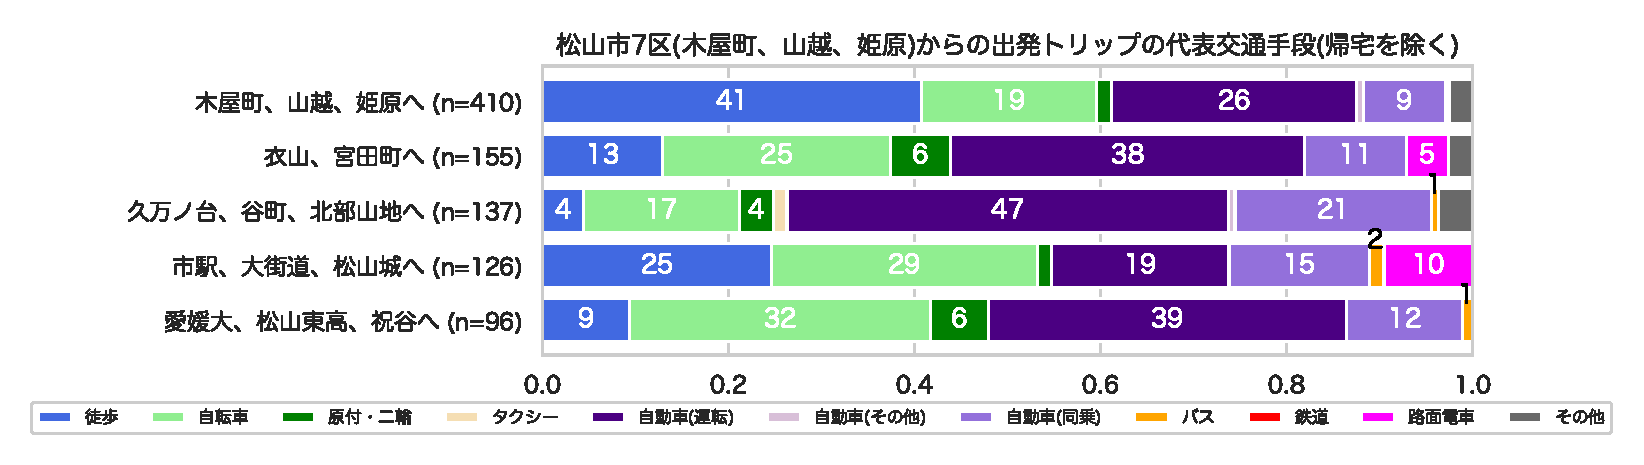
\includegraphics[width=1.0\textwidth]{picture/mode_share_松山市7区.eps}
    \caption{松山市7区を出発するトリップの交通手段割合}
    \label{fig:mode_share_7}
\end{figure}

\subsubsection{松山市8区 (湯の山、北東山地)}
自転車の分担率が他の地域と比較して著しく低く、自動車や原付・二輪の分担率が高い。
これは、山地部で坂が多いためと考えられる。
バスによる移動が、松山市6区 (衣山、宮田町)への移動の8\%、松山市3区 (愛媛大、松山東高校、祝谷)への移動の4\%を占めており、自動車や自転車による移動が困難な人の重要な移動手段となっていると考えられる。
%
\begin{figure}[H]
    \centering
    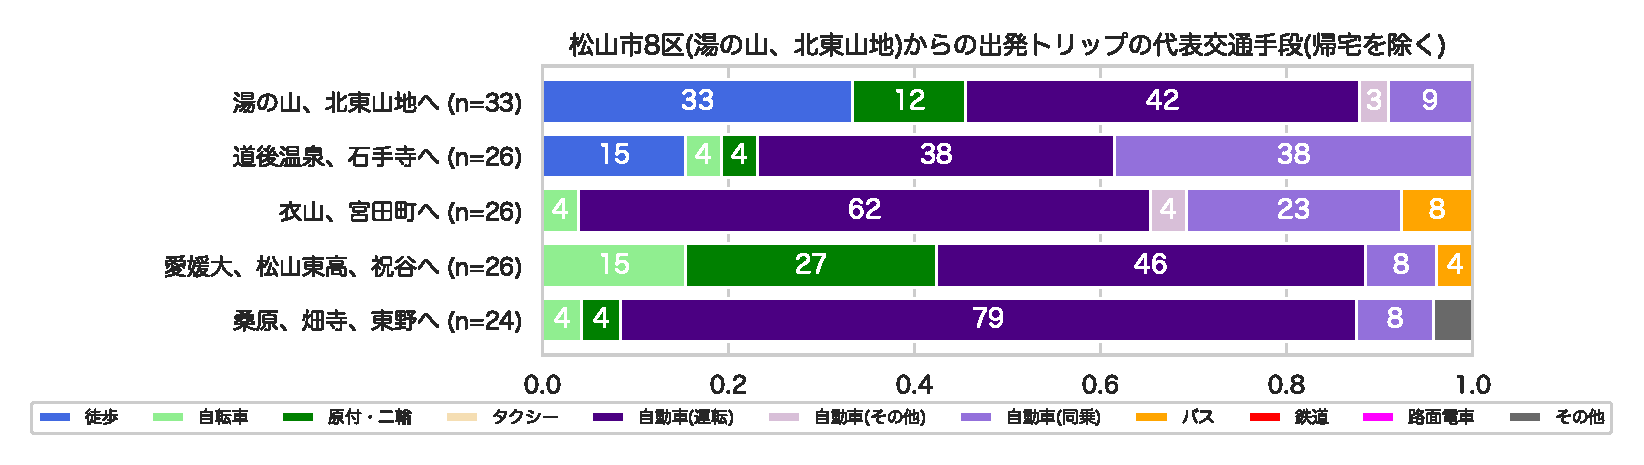
\includegraphics[width=1.0\textwidth]{picture/mode_share_松山市8区.eps}
    \caption{松山市8区を出発するトリップの交通手段割合}
    \label{fig:mode_share_8}
\end{figure}

\subsubsection{松山市9区 (平井、梅本、東久米)}
郊外部にあたる松山市9区では、地区内移動の徒歩と自転車の割合がさらに減少し、自動車に代替される (5割程度)。
また、東温市1区 (横河原駅、愛大医学部)や松山市11区 (久米、南土居、高井)、松山市14区 (市坪、松山IC、森松)といった周辺地域への移動はおよそ8割を自動車による移動が占める。
他地域と比較すると自転車の分担率が著しく低いため、歩道・自転車道の整備や駅の駐輪場整備により、自転車走行環境や乗り換え利便性を高める必要があると考えられる。
%
\begin{figure}[H]
    \centering
    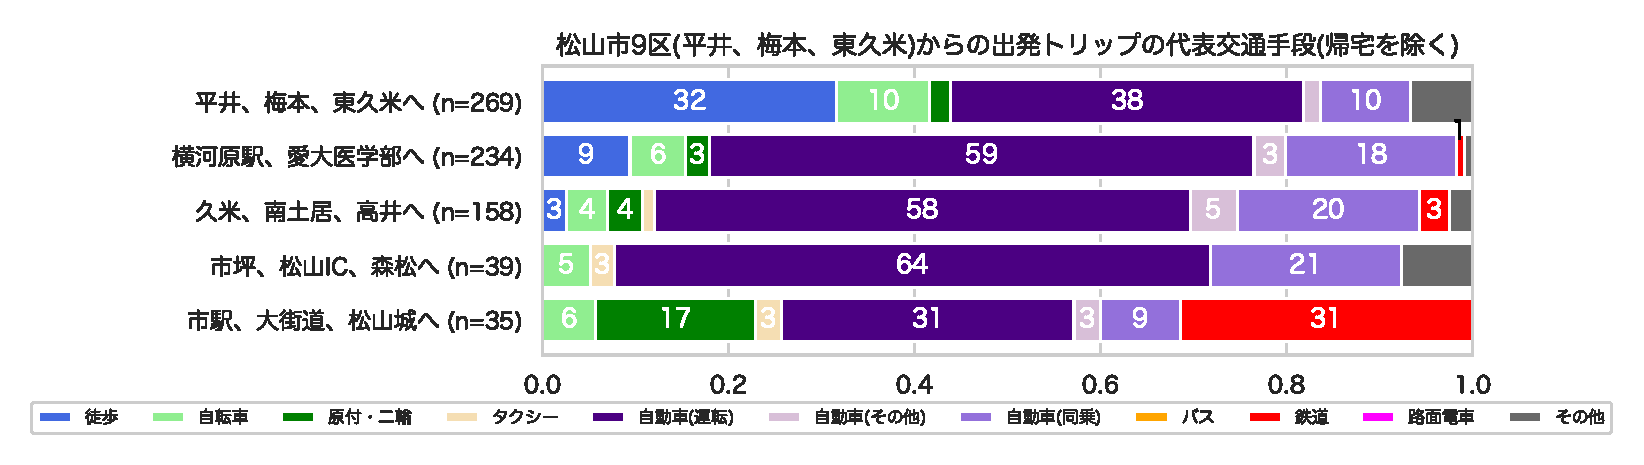
\includegraphics[width=1.0\textwidth]{picture/mode_share_松山市9区.eps}
    \caption{松山市9区を出発するトリップの交通手段割合}
    \label{fig:mode_share_9}
\end{figure}

\subsubsection{松山市10区 (桑原、畑寺、東野)}
松山市1区 (市駅、大街道、松山城)や松山市3区 (愛媛大、松山東高校、祝谷)への移動に占める自転車・原付 (35〜36\%)とバス (6〜11\%)の割合が高い。
中心部への移動に、バスと二輪が日常的な交通手段となっていると言えるため、自転車やバスの利便性をさらに向上させることで利用者の増加を見込める。
一方で、松山市11区 (久米、南土居、高井)や松山市4区 (いよ立花駅、朝生田)への郊外部どうしの移動は、自動車による移動が大半である。
%
\begin{figure}[H]
    \centering
    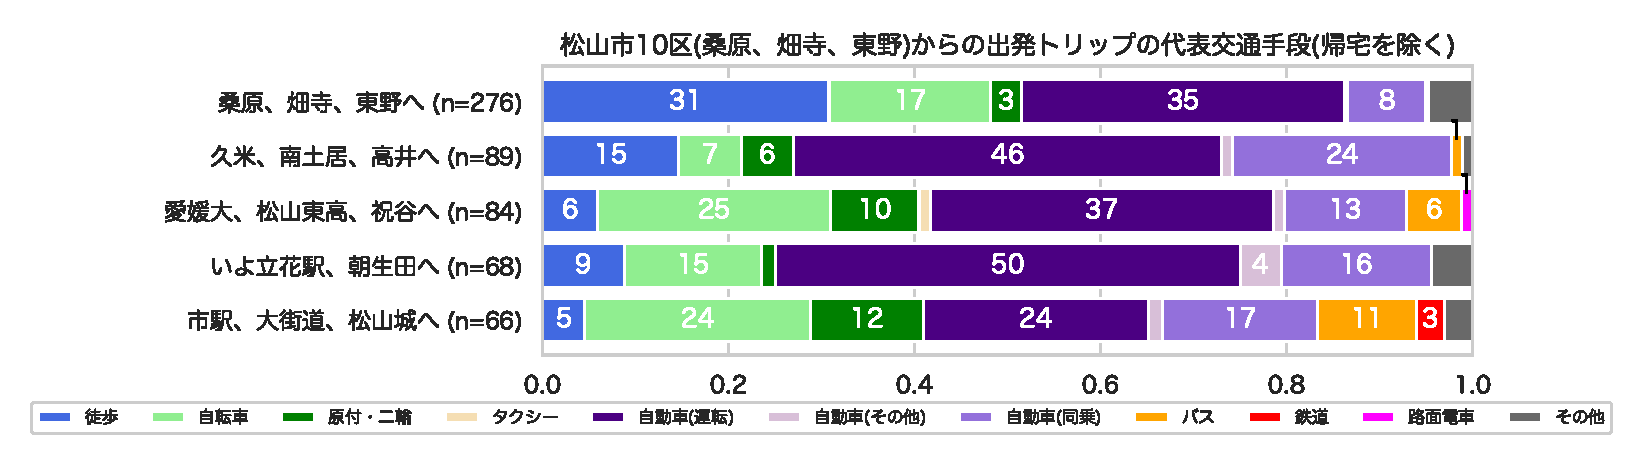
\includegraphics[width=1.0\textwidth]{picture/mode_share_松山市10区.eps}
    \caption{松山市10区を出発するトリップの交通手段割合}
    \label{fig:mode_share_10}
\end{figure}

\subsubsection{松山市11区 (久米、南土居、高井)}
松山市9区 (平井、梅本、東久米)と同じ傾向で、地区内移動の徒歩と自動車の割合が55\%を占め、周辺地域への移動はおよそ8〜9割を自動車による移動が占める。
また、周辺地域への移動のバスや鉄道の分担率が著しく低く、別の人の運転する自動車への同乗の割合が他地域と比較して高い。
土居や高井には、公共交通の空白地帯の新興住宅地が存在し、スプロール化した宅地であるがゆえに買い物や公共施設への距離も遠く、住民が自動車以外の選択肢を持たないと推察される。
したがって、公共交通空白地帯と周辺地域・駅をつなぐバス路線の新設、バイクシェアの導入、駅の駐車場・駐輪場整備による乗り換え利便性の向上、歩道・自転車道の整備による自転車走行環境の改善等の施策を行い、自動車に頼らない移動を実現する必要がある。
%
\begin{figure}[H]
    \centering
    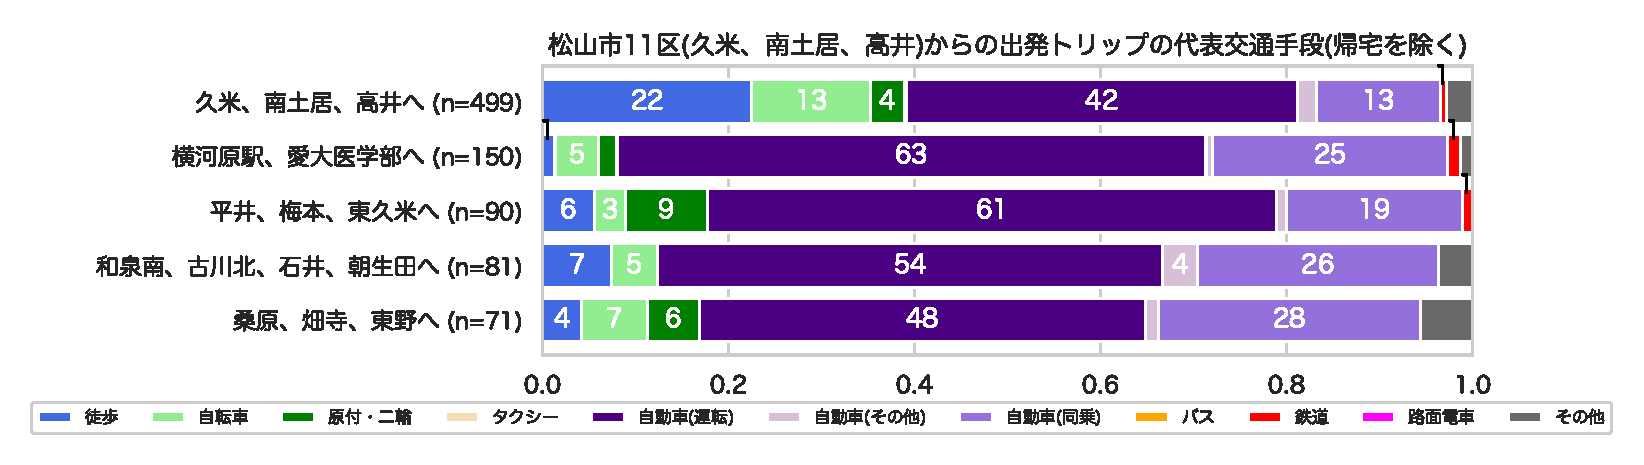
\includegraphics[width=1.0\textwidth]{picture/mode_share_松山市11区.eps}
    \caption{松山市11区を出発するトリップの交通手段割合}
    \label{fig:mode_share_11}
\end{figure}

\subsubsection{松山市12区 (久谷、荏原、浄瑠璃)}
山間部の地域であり、自動車による移動が大半を占める。
%
\begin{figure}[H]
    \centering
    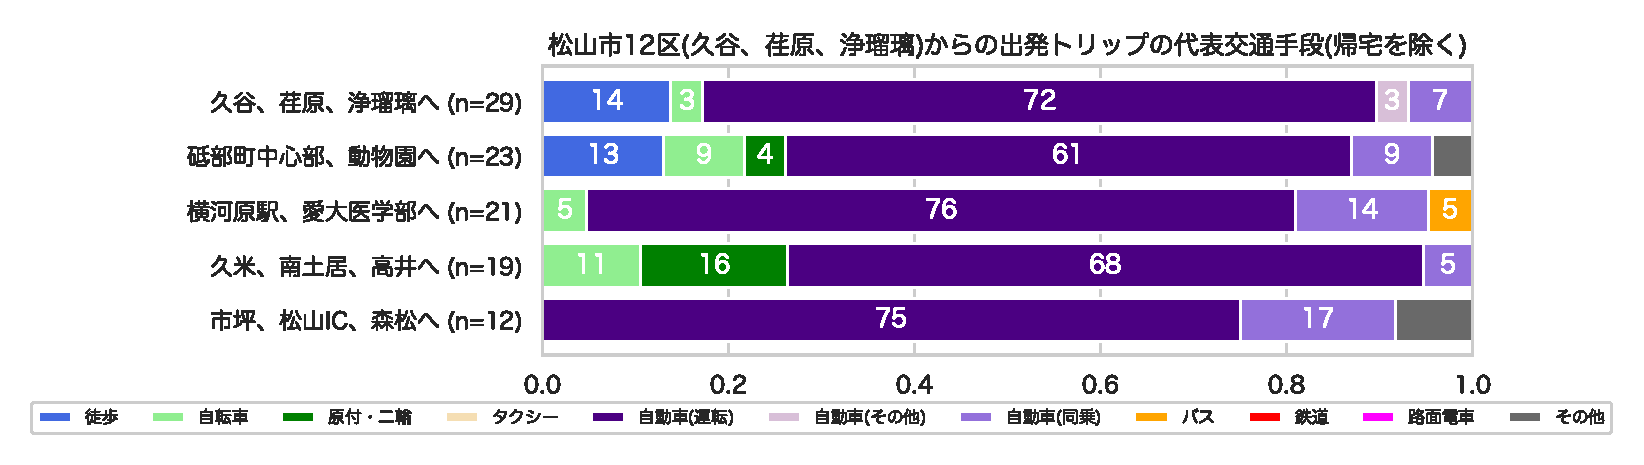
\includegraphics[width=1.0\textwidth]{picture/mode_share_松山市12区.eps}
    \caption{松山市12区を出発するトリップの交通手段割合}
    \label{fig:mode_share_12}
\end{figure}

\subsubsection{松山市13区 (和泉南、古川北、石井、朝生田)}
他の郊外部と同じく、自動車中心の移動構成で、松山市10区 (桑原、畑寺、東野)と類似している。
隣接する松山市11区 (久米、南土居、高井)や松山市14区 (市坪、松山IC、森松)への移動需要が多いが、公共交通は利用されていない。
松山市11区 (久米、南土居、高井)と同じく、公共交通の空白地帯の新興住宅地が存在するため、そのような地域の新規路線の整備や、近隣のいよ立花駅、福音寺駅、JR市坪駅におけるパークアンドライド・サイクルアンドライドによる乗り換え利便性の向上が必要であろう。
%
\begin{figure}[H]
    \centering
    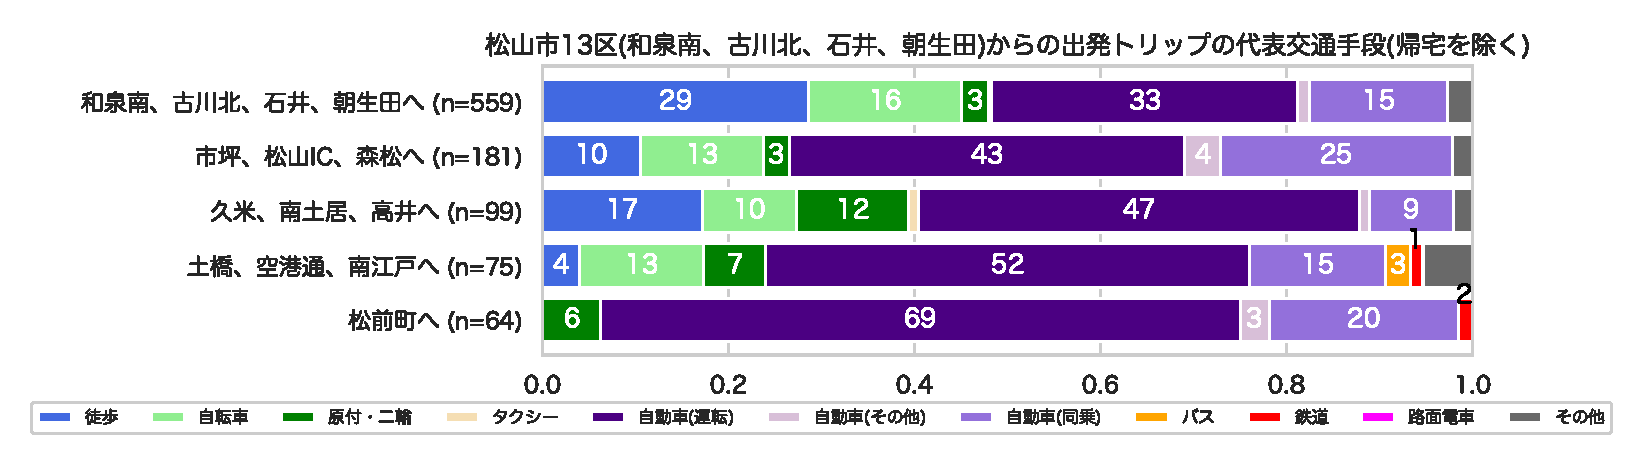
\includegraphics[width=1.0\textwidth]{picture/mode_share_松山市13区.eps}
    \caption{松山市13区を出発するトリップの交通手段割合}
    \label{fig:mode_share_13}
\end{figure}

\subsubsection{松山市14区 (市坪、松山IC、森松)}
松山市13区 (和泉南、古川北、石井、朝生田)と同様の手段構成である。
一方で、特徴的な構成として、松山市1区 (市駅、大街道、松山城)への移動のうち、20\%をバスが占める点が挙げられる。
バス利用のポテンシャルは高いため、松山市13区 (和泉南、古川北、石井、朝生田)や松山市11区 (久米、南土居、高井)とをつなぐバス路線が有望である。
%
\begin{figure}[H]
    \centering
    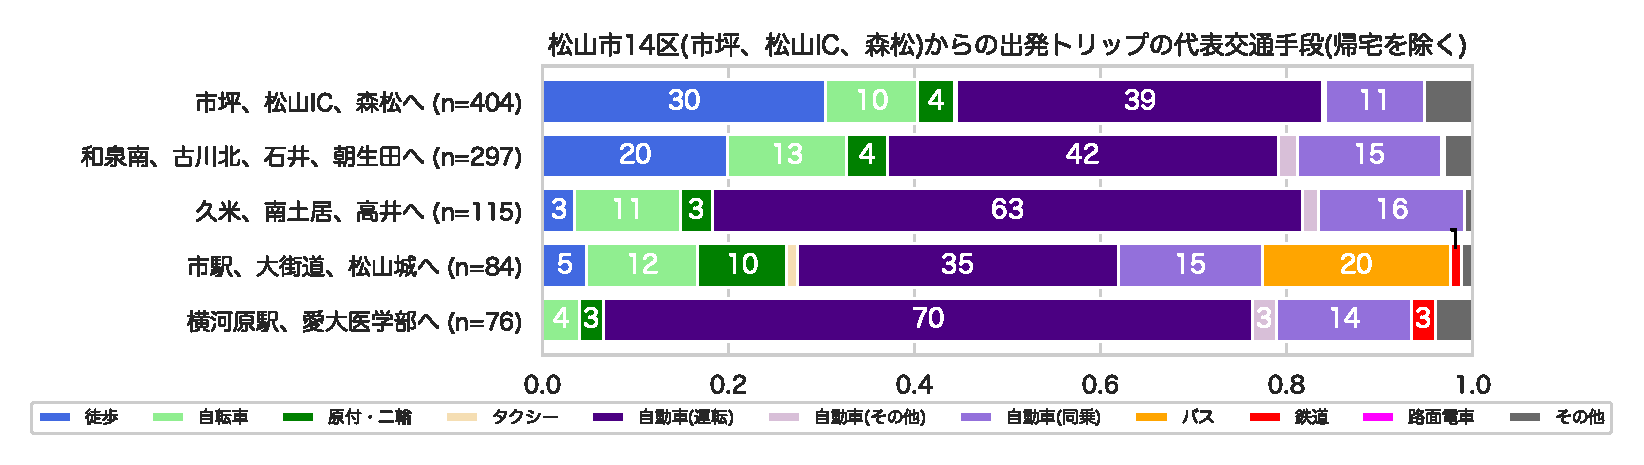
\includegraphics[width=1.0\textwidth]{picture/mode_share_松山市14区.eps}
    \caption{松山市14区を出発するトリップの交通手段割合}
    \label{fig:mode_share_14}
\end{figure}

\subsubsection{松山市15区 (垣生、余戸、土居田)}
伊予鉄郡中線の中間部に位置しており、松山市5区 (土橋、空港通り、南江戸)、松前町、松山市1区 (市駅、大街道、松山城)への移動に占める鉄道分担率が比較的高いことが特徴である。
特に、松山市1区 (市駅、大街道、松山城)への移動の32\%を鉄道が占めており、松山市9区 (平井、梅本、東久米)と同様に、伊予鉄郊外線が中心部に向けた移動の主要な交通手段となっている。
ただし、松山市13区 (和泉南、古川北、石井、朝生田)や松山市14区 (市坪、松山IC、森松)と同じく、周辺地域への移動は自動車の利用が6〜8割を占めるため、自転車や公共交通の分担率を向上させる取り組みが必要である。
特に、公共交通は既存の路線を活用するため、駅での乗り換え利便性の向上や待ち時間の表示、コミュニケーションによる利用促進策が有効であろう。
%
\begin{figure}[H]
    \centering
    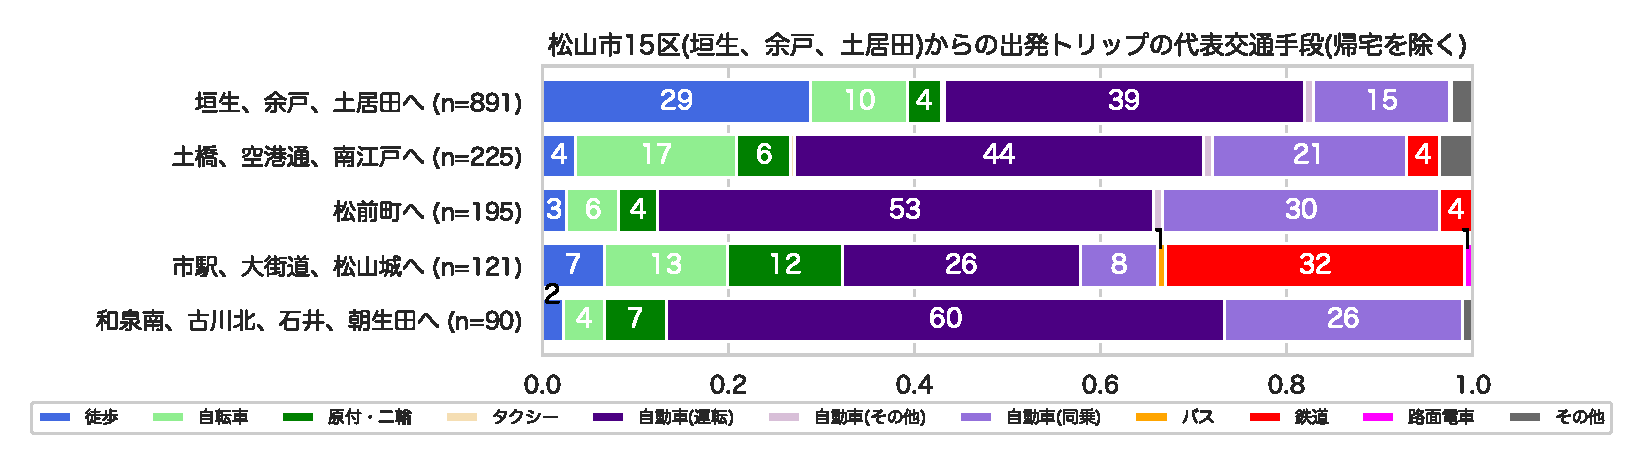
\includegraphics[width=1.0\textwidth]{picture/mode_share_松山市15区.eps}
    \caption{松山市15区を出発するトリップの交通手段割合}
    \label{fig:mode_share_15}
\end{figure}

\subsubsection{松山市16区 (北斎院、南斎院、北吉田)}
他の郊外部と比較すると、自動車の分担率が低く、徒歩と自転車の分担率が高い。
%
\begin{figure}[H]
    \centering
    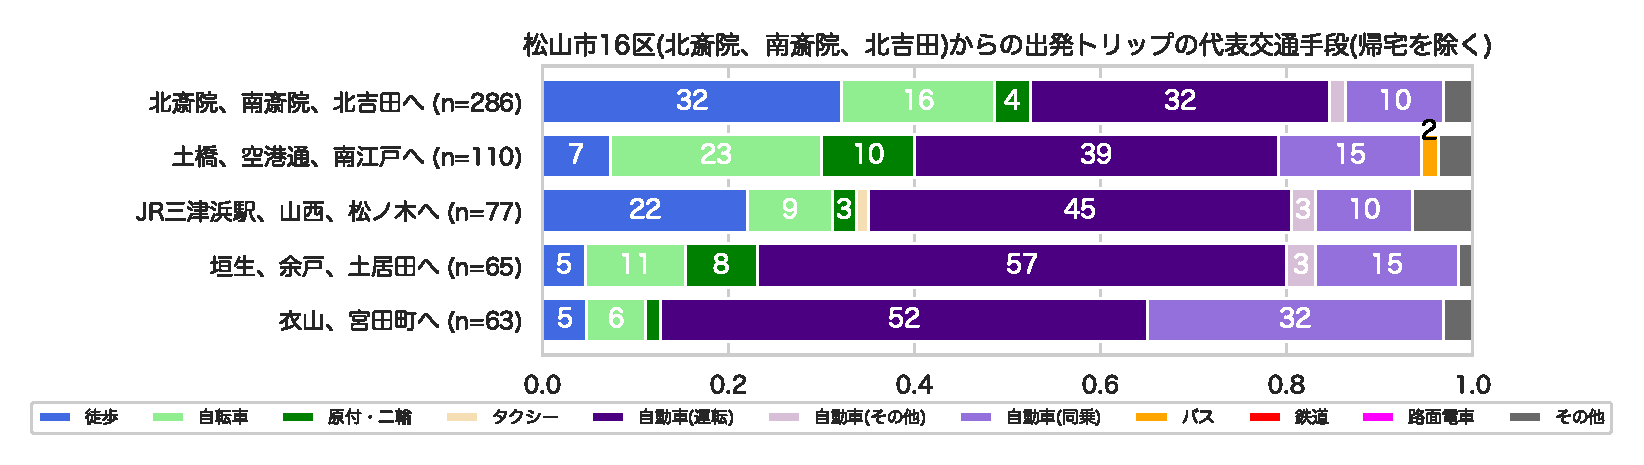
\includegraphics[width=1.0\textwidth]{picture/mode_share_松山市16区.eps}
    \caption{松山市16区を出発するトリップの交通手段割合}
    \label{fig:mode_share_16}
\end{figure}

\subsubsection{松山市17区 (JR三津浜駅、山西、松ノ木)}
松山市13区 (和泉南、古川北、石井、朝生田)、松山市14区 (市坪、松山IC、森松)、松山市15区 (垣生、余戸、土居田)と同様の手段構成である。
松山市15区 (垣生、余戸、土居田)と同様に、松山市1区 (市駅、大街道、松山城)への移動の22\%を鉄道が占めており、伊予鉄郊外線が中心部に向けた移動の主要な交通手段となっている。
一方で、松山市6区 (衣山、宮田町)への移動の鉄道の分担率は4\%にとどまり、鉄道利用の促進が必要である。
%
\begin{figure}[H]
    \centering
    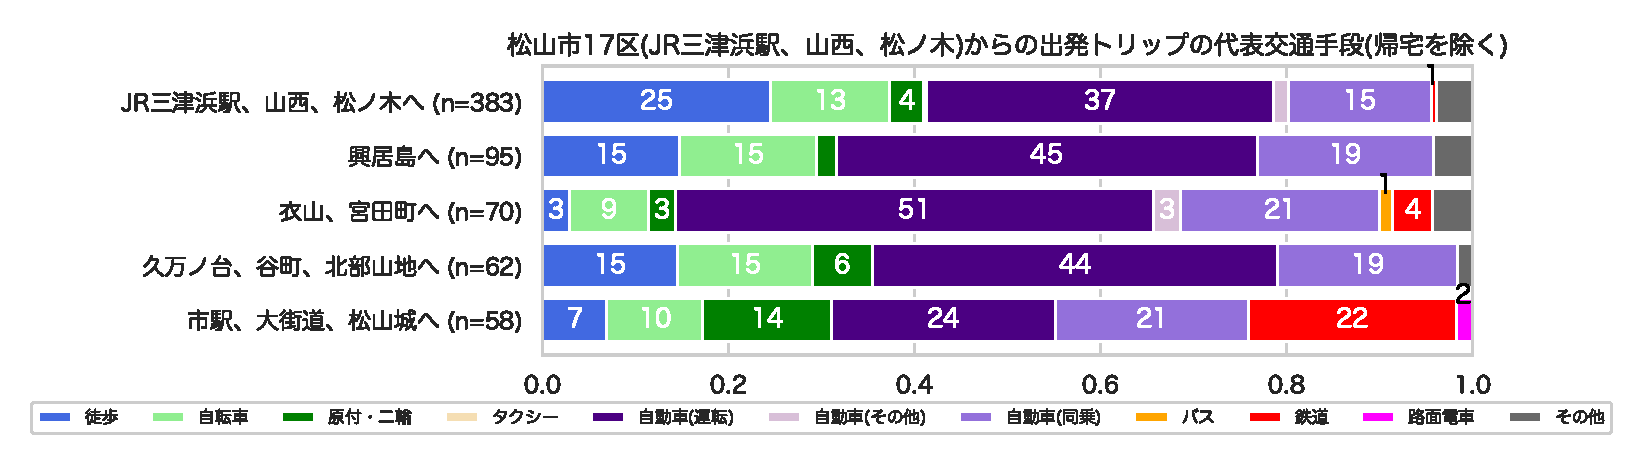
\includegraphics[width=1.0\textwidth]{picture/mode_share_松山市17区.eps}
    \caption{松山市17区を出発するトリップの交通手段割合}
    \label{fig:mode_share_17}
\end{figure}

\subsubsection{松山市18区 (久万ノ台、谷町、北部山地)}
松山市17区 (JR三津浜駅、山西、松ノ木)と同様に、周辺地域への移動は自動車が主要な交通手段であるが、松山市1区 (市駅、大街道、松山城)への移動はバスが12\%、鉄道が6\%を占めている。
他地域と比較して、バスの利用が多く、坂のある地形において自動車を運転できない人の移動をバスが支えていると考えられる。
%
\begin{figure}[H]
    \centering
    \includegraphics[width=1.0\textwidth]{picture/mode_share_松山市18区.eps}
    \caption{松山市18区を出発するトリップの交通手段割合}
    \label{fig:mode_share_18}
\end{figure}

\subsubsection{松山市19区 (伊予和気、堀江)}
松山市17区 (JR三津浜駅、山西、松ノ木)と同様に、周辺地域への移動は自動車が主要な交通手段であるが、松山市1区 (市駅、大街道、松山城)への移動はバスが12\%、鉄道が4\%を占めている。
自転車の分担率が低く、生活圏域が広いことや地形が影響していると考えられる。
%
\begin{figure}[H]
    \centering
    \includegraphics[width=1.0\textwidth]{picture/mode_share_松山市19区.eps}
    \caption{松山市19区を出発するトリップの交通手段割合}
    \label{fig:mode_share_19}
\end{figure}

\subsubsection{松山市20区 (高浜、興居島)}
トリップ数は少ないものの、松山市1区 (市駅、大街道、松山城)への移動や、松山市6区 (衣山、宮田町)への移動に占める公共交通の割合が高い。
松山市17区 (JR三津浜駅、山西、松ノ木)と同様に、伊予鉄の郊外線が中心部への主要な交通手段となっている。
%
\begin{figure}[H]
    \centering
    \includegraphics[width=1.0\textwidth]{picture/mode_share_松山市20区.eps}
    \caption{松山市20区を出発するトリップの交通手段割合}
    \label{fig:mode_share_20}
\end{figure}

\subsubsection{松山市21区 (空港)}
データ数が少ないものの、他の郊外地域と傾向は概ね同様である。
松山都市圏の住民のデータのみであるため、飛行機で松山空港へ到着した松山都市圏外の人のデータは存在しないことに注意が必要である。
%
\begin{figure}[H]
    \centering
    \includegraphics[width=1.0\textwidth]{picture/mode_share_松山市21区.eps}
    \caption{松山市21区を出発するトリップの交通手段割合}
    \label{fig:mode_share_21}
\end{figure}

\subsubsection{松山市22区 (道後温泉、石手寺)}
データが少ないものの、周辺地域の移動に占める路面電車の割合が高いことが特徴である。
また、徒歩と自転車の分担率が高く、中心部同様、ウォーカブルな環境と言える。
%
\begin{figure}[H]
    \centering
    \includegraphics[width=1.0\textwidth]{picture/mode_share_松山市22区.eps}
    \caption{松山市22区を出発するトリップの交通手段割合}
    \label{fig:mode_share_22}
\end{figure}

\subsubsection{松山市27区 (北条)}
北条地域は、徒歩と自転車の分担率が低く、自動車の分担率が高い。
多くのトリップは北条のゾーン内で行われるため、地域内のデマンド交通やバイクシェアが、公共交通中心の街づくりに有効であると考えられる。
%
\begin{figure}[H]
    \centering
    \includegraphics[width=1.0\textwidth]{picture/mode_share_松山市27区.eps}
    \caption{松山市27区を出発するトリップの交通手段割合}
    \label{fig:mode_share_27}
\end{figure}

\subsubsection{伊予市1区 (郡中、伊予市駅)}
地区内の移動、および松前町への移動が多いが、その65〜87\%が自動車よる移動である。
松山市内の郊外部よりさらに自動車中心のライフスタイルが構築されていると言える。
松山市15区 (垣生、余戸、土居田)や松山市1区 (市駅、大街道、松山城)への移動は、バスや鉄道といった公共交通が使われる傾向にあるが、絶対数は少ない。
%
\begin{figure}[H]
    \centering
    \includegraphics[width=1.0\textwidth]{picture/mode_share_伊予市1区.eps}
    \caption{伊予市1区を出発するトリップの交通手段割合}
    \label{fig:mode_share_iyo1}
\end{figure}

\subsubsection{東温市1区 (横河原駅、愛大医学部)}
伊予市1区 (郡中、伊予市駅)と同様に、地区内移動の自動車の分担率が78\%と非常に高い。
松山市11区 (久米、南土居、高井)や松山市9区 (平井、梅本、東久米)といった周辺地域の移動も見られるが、そのほとんどが自動車による移動であり、
松山市11区 (久米、南土居、高井)への移動の95\%、松山市9区 (平井、梅本、東久米)への移動の90\%を占める。
過度な自動車依存を低減するため、横河原駅や見奈良駅におけるパークアンドライドやサイクルアンドライドの施策が必要であろう。
また、目的地である、久米、梅本、平井、鷹ノ子駅におけるシェアバイク等の端末交通も重要である。
%
\begin{figure}[H]
    \centering
    \includegraphics[width=1.0\textwidth]{picture/mode_share_東温市1区.eps}
    \caption{東温市1区を出発するトリップの交通手段割合}
    \label{fig:mode_share_toon1}
\end{figure}

\subsubsection{松前町}
伊予市や東温市と同じく、ほとんどの移動は自動車で行われ、徒歩・自転車・公共交通の分担率は著しく低い。
東温市と同じく、過度な自動車依存を低減するため、バスの利便性向上や松前駅におけるパークアンドライドやサイクルアンドライドの実施、目的地である郡中駅や余戸駅におけるシェアバイク等の端末交通の整備が必要である。
%
\begin{figure}[H]
    \centering
    \includegraphics[width=1.0\textwidth]{picture/mode_share_松前町.eps}
    \caption{松前町を出発するトリップの交通手段割合}
    \label{fig:mode_share_masaki}
\end{figure}

\subsubsection{砥部町1区 (砥部町中心部、動物園)}
伊予市、東温市、松前町と同じく、ほとんどの移動は自動車で行われ、徒歩・自転車・公共交通の分担率は著しく低い。
バスの利便性向上や自転車利用の促進が重要である。
%
\begin{figure}[H]
    \centering
    \includegraphics[width=1.0\textwidth]{picture/mode_share_砥部町1区.eps}
    \caption{砥部町1区を出発するトリップの交通手段割合}
    \label{fig:mode_share_tobe1}
\end{figure}


\color{red}
\begin{framed}
\noindent
\textbf{\large 松山市中心部を出発する移動は、近距離移動は徒歩・自転車、中距離移動は公共交通、公共交通不便地域への移動は自動車が使われる傾向にあり、徒歩・自転車・公共交通中心の街が形成されている。
また、伊予鉄郊外線沿線の地域では、松山市中心部までの移動に鉄道がよく利用されており、乗り換え利便性の向上により更なる利用者増加を目指す施策が有効である。
その一方で、郊外部と郊外部の間の移動や、郊外の新興住宅地、松山市の周辺の市町村、山間部では、ほとんどの移動が自動車によって占められている。
需要の多い地区間移動には、バスの新規路線の検討、拠点駅の駐輪場・駐車場・待合施設の整備による乗り換え利便性向上、バイクシェアの導入、歩道・自転車道の整備といった施策により、自動車利用を徒歩・自転車・公共交通に少しずつ転換していく必要がある。
}
\end{framed}
\color{black}


\clearpage
\section{移動時間の分析}
各地区の目的別の移動時間について分析する。
図\ref{fig:time_commute}は、各地区を出発する通勤トリップの移動時間を示した図である。
赤線が中央値、箱の左端と右端がそれぞれ第一四分位点、第三四分位点を示す。
ほとんどの地域において、通勤トリップの移動時間の中央値は20分以内で、75\%のトリップは30分以内に完了する。
一方で、松山市8区 (湯の山、北東山地)、松山市12区 (久谷、荏原、浄瑠璃)、松山市19区 (伊予和気、堀江)、松山市22区 (道後温泉、石手寺)、松山市27区 (北条)エリアでは、中央値や第三四分位点が10分程度長い。
%
\begin{figure}[H]
    \centering
    \includegraphics[width=1.0\textwidth]{picture/time_通勤.eps}
    \caption{各地区を出発する通勤トリップの移動時間}
    \label{fig:time_commute}
\end{figure}

\clearpage
図\ref{fig:time_school}は、各地区を出発する通学トリップの移動時間を示す。
通勤と比較すると、校区制により広範囲の移動は少ないため、同一地区内の移動時間の分散は小さい。
一方で、地区間の差異は大きく、松山市8区 (湯の山、北東山地)、松山市12区 (久谷、荏原、浄瑠璃)、松山市27区 (北条)、伊予市1区 (郡中、伊予市駅)、東温市1区 (横河原駅、愛大医学部)の移動時間は、他の地区に比べて10〜20分程度大きい。
%
\begin{figure}[H]
    \centering
    \includegraphics[width=1.0\textwidth]{picture/time_通学.eps}
    \caption{各地区を出発する通学トリップの移動時間}
    \label{fig:time_school}
\end{figure}

図\ref{fig:time_shopping}は、各地区を出発する買い物トリップの移動時間を示す。
移動時間の中央値は20分以内であり、通勤と比較すると近場で移動が行われている。
一方で、通勤・通学で移動時間の長かった地域で、同様に買い物の移動時間も長くなっている。
%
\begin{figure}[H]
    \centering
    \includegraphics[width=1.0\textwidth]{picture/time_買い物.eps}
    \caption{各地区を出発する買い物トリップの移動時間}
    \label{fig:time_shopping}
\end{figure}

\clearpage
図\ref{fig:time_leisure}は、各地区を出発する食事・社交・娯楽トリップの移動時間を示す。
松山市1区 (市駅、大街道、松山城)、松山市2区 (大手町、本町、味酒)、松山市6区 (衣山、宮田町)、松山市7区 (木屋町、山越、姫原)、松山市8区 (湯の山、北東山地)、松山市13区 (和泉南、古川北、石井、朝生田)といった地域で移動時間が短く、中心市街地や郊外のショッピングセンター、ロードサイド店舗への利便性が高いためと考えられる。
%
\begin{figure}[H]
    \centering
    \includegraphics[width=1.0\textwidth]{picture/time_食事・社交・娯楽.eps}
    \caption{各地区を出発する食事・社交・娯楽トリップの移動時間}
    \label{fig:time_leisure}
\end{figure}

\color{red}
\begin{framed}
\noindent
\textbf{\large 山間部を中心に、移動に時間を要する、移動不便地域が存在する。
}
\end{framed}
\color{black}

\clearpage
\section{駐車場の利用状況}
本パーソントリップ調査では、自動車によるトリップの場合、到着地の駐車場の種類や駐車料金のデータを取得している。
無料駐車場、時間貸駐車場、月極駐車場の種類ごとに、目的地や施設種類に関して分析する。

図\ref{fig:facility_share_parking}は、各駐車場を利用する際の目的施設の割合を示している (住宅・寮を除く)。
まず、駐車場を利用する場合のほとんどが無料駐車場である。
無料駐車場を利用する際の目的施設は、飲食店、官公庁、大型商店が特に多い。
時間貸駐車場は、より多様な施設種別を目的地とする場合に利用される。
特に、事務所・会社・銀行、官公庁、農林漁業作業など業務系施設や医療施設を訪れる際の利用が多い。
月極駐車場は、官公庁の利用に多い。
%
\begin{figure}[H]
    \centering
    \includegraphics[width=1.0\textwidth]{picture/facility_share_parking.eps}
    \caption{各駐車場を利用する際の目的施設 (住宅・寮を除く)}
    \label{fig:facility_share_parking}
\end{figure}

\clearpage
次に、目的地の施設別に駐車場の種類の割合を、図\ref{fig:parking_share_facility}に示す。
ほとんどが無料駐車場であるが、文化・宗教施設、公園・緑地、体育・レクリエーション施設の利用時には、およそ1割程度時間貸駐車場の利用が見られる。
%
\begin{figure}[H]
    \centering
    \includegraphics[width=1.0\textwidth]{picture/parking_share_facility.eps}
    \caption{各施設を利用する際の駐車場の種別}
    \label{fig:parking_share_facility}
\end{figure}

\clearpage
目的地別の駐車場の種類の割合を、図\ref{fig:parking_share_zone}に示す。
松山市1区 (市駅、大街道、松山城)、松山市2区 (大手町、本町、味酒)、松山市3区 (愛媛大、松山東高校、祝谷)を訪れる際は、時間貸駐車場の割合がおよそ1割を占めており、他の地域と比較して高い。
他に、松山市12区 (久谷、荏原、浄瑠璃)、松山市22区 (道後温泉、石手寺)を訪れる際も、時間貸駐車場が多い。
%
\begin{figure}[H]
    \centering
    \includegraphics[width=1.0\textwidth]{picture/parking_share_zone.eps}
    \caption{各地区を自動車で訪れる際の駐車場の種別}
    \label{fig:parking_share_zone}
\end{figure}

\clearpage
特に時間貸駐車場の利用が多い、中心部に買い物・娯楽目的で訪れるトリップに着目して駐車料金を調べる。
図\ref{fig:parking_fee}は駐車料金分布、図\ref{fig:parking_fee_per_hour}は滞在時間で割った時間あたりの駐車料金分布である。
ほとんどの場合、駐車料金は1000円以下で、400円以下の場合が多い。
時間あたりに直すと、200円程度である。
%
\begin{figure}[H]
    \centering
    \includegraphics[width=0.7\textwidth]{picture/parking_fee.eps}
    \caption{中心部に買い物・娯楽目的で訪れるトリップの駐車料金分布}
    \label{fig:parking_fee}
\end{figure}
%
\begin{figure}[H]
    \centering
    \includegraphics[width=0.7\textwidth]{picture/parking_fee_per_hour.eps}
    \caption{中心部に買い物・娯楽目的で訪れるトリップの時間あたりの駐車料金分布}
    \label{fig:parking_fee_per_hour}
\end{figure}

\color{red}
\begin{framed}
\noindent
\textbf{\large 車で移動する際の駐車場はほとんどの場合無料である。一方で、中心部の移動や業務・娯楽施設を目的地として移動で、時間貸駐車場の利用が1割程度見られる。
}
\end{framed}
\color{black}


\clearpage
\section{端末交通と交通手段の組み合わせ}
複数の交通手段を組み合わせた移動に関して検討するため、2つ以上の交通手段を組み合わせたトリップについて分析する。
図\ref{fig:transit_combination}は、2つ以上の交通手段の組み合わせパターンのうち、上位10組を表す (帰宅を除く)。
徒歩と鉄道・バス・路面電車・自動車の組み合わせが多くを占める。
パークアンドライドやサイクルアンドライドと呼ばれる、自動車と鉄道、自転車と鉄道の組み合わせはほぼ存在しない。
%
\begin{figure}[H]
    \centering
    \includegraphics[width=1.0\textwidth]{picture/transit_combination.eps}
    \caption{2つ以上の交通手段の組み合わせ (上位10組。帰宅を除く)}
    \label{fig:transit_combination}
\end{figure}

\color{red}
\begin{framed}
\noindent
\textbf{\large 自転車・自動車と公共交通を組み合わせた移動はほとんど見られない。拠点駅において駐輪場や無料駐車場を整備することにより、公共交通の利用を促進する施策が有効と考えられる。
}
\end{framed}
\color{black}

\clearpage
\chapter{主体に着目した移動の分析}
この章では、松山都市圏に住む特定の住民の属性に着目して、生活パターン、移動の目的地、交通手段、買い物・娯楽トリップを分析する。
具体的には、19〜25歳の若年層、中学生・高校生、70歳以上の高齢者、免許返納者 (70歳以上)、子育て世帯の親、在宅勤務者 (25〜59歳)、低所得世帯 (59歳以下)、外出に困難のある人について分析し、移動・活動の特徴を見出す。

\section{19〜25歳の若年層}

表\ref{tab:トリップ_外出率_若年層}は、19〜25歳の若年層のトリップ原単位と外出率を示す。
19〜25歳の若年層のグロス原単位 (外出していない人も含む1日の移動回数)は、平日・休日とも人口全体より小さい。
平日の外出率は、人口全体の平均と比較して大きいが、外出した人の平均トリップ数 (ネット原単位)が小さい。
また、休日の外出率は、50\%を割り込んでおり、人口全体と比較して小さい。
まちの賑わいを回復させるためには、若年層の休日の外出を引き出すようなまちづくりが求められる。
%
\begin{table}[htbp]
\centering
\caption{トリップ原単位と外出率 (19〜25歳の若年層)}
\label{tab:トリップ_外出率_若年層}
\begin{tabular}{lrr}
\toprule
& 若年層 & 人口全体 \\
\midrule
拡大前人数 (トリップ数) & 659 (2209) & 19021 (60043)\\
トリップ原単位(グロス) & & \\
\hspace{2em} 平日 & 1.88 & 1.97 \\
\hspace{2em} 休日 & 1.31 & 1.60 \\
トリップ原単位(ネット) & & \\
\hspace{2em} 平日 & 2.44 & 2.72 \\
\hspace{2em} 休日 & 2.65 & 2.88\\
外出率 (\%) & & \\
\hspace{2em} 平日 & 76.9 & 72.2\\
\hspace{2em} 休日 & 49.3 & 55.6\\
\bottomrule
\end{tabular}
\end{table}

次に、19〜25歳の若年層の平日・休日のアクティビティパターンを図\ref{fig:activity_pattern_young}に示す。
平日は、移動なしが24\%、家と職場・学校の往復のみが54\%を占めており、食事・買い物・娯楽を含むその他の移動は22\%のみである。
休日は、移動しない人が51\%を占め、食事・買い物・娯楽とその他の移動は31\%のみである。
したがって、若年層の平日の立ち寄り行動や休日の外出を促すような施設整備や街づくりが求められる。
%
\begin{figure}[htbp]
    \centering
    \includegraphics[width=1.0\textwidth]{picture/activity_pattern_若年層.eps}
    \caption{若年層のアクティビティパターン}
    \label{fig:activity_pattern_young}
\end{figure}

19〜25歳の若年層の通勤・通学の出発地と目的地の分布を図\ref{fig:od_commute_young}に示す。
上図が若年層、下図が全体を表す。
通勤・通学トリップは、愛媛大学や松山大学の立地する松山市3区へと集中している。
また、松山市3区に向けては、松山市3区に加えて、松山市7区 (木屋町、山越、姫原)、松山市10区 (桑原、畑寺、東野)、松山市15区 (垣生、余戸、土居田)からのトリップが多い。
%
\begin{figure}[htbp]
  \centering
  \subfigure[若年層]{%
    \includegraphics[clip, width=0.7\columnwidth]{picture/connection_若年層_通勤・通学.eps}}\\%
  \subfigure[全体]{%
    \includegraphics[clip, width=0.7\columnwidth]{picture/connection_通勤・通学.eps}}
    \caption{通勤・通学目的の出発地 (左列)と到着地 (右列)}
  	\label{fig:od_commute_young}
\end{figure}

19〜25歳の若年層の買い物の出発地と目的地の分布を図\ref{fig:od_shopping_young}に示す。
人口全体と比較して、松山市1区 (市駅、大街道、松山城)と松前町を利用する割合が高い。
前者は大学に近い中心市街地、後者は大型ショッピングモールの存在が、選択の理由として挙げられる。
%
\begin{figure}[htbp]
  \centering
  \subfigure[若年層]{%
    \includegraphics[clip, width=0.7\columnwidth]{picture/connection_若年層_買い物.eps}}\\%
  \subfigure[全体]{%
    \includegraphics[clip, width=0.7\columnwidth]{picture/connection_買い物.eps}}
    \caption{買い物目的の出発地 (左列)と到着地 (右列)}
  	\label{fig:od_shopping_young}
\end{figure}

図\ref{fig:od_leisure_young}に示す、食事・社交・娯楽・観光のトリップの目的地は、人口全体と概ね似た傾向であるが、松山市11区 (久米、南土居、高井)や松山市14区 (市坪、松山IC、森松)といったロードサイド店舗の多い地区が少なく、松山市1区 (市駅、大街道、松山城)や松山市22区 (道後温泉、石手寺)といった中心市街地と、東温市1区 (横河原駅、愛媛大学医学部)や松前町といった郊外のショッピングモールのある地区への移動が多い。
これらのことから、すでに余暇活動の目的地として選ばれている中心部の魅力を高めることで、若年層の外出率や移動をさらに増加させることができると考えられる。
%
\begin{figure}[htbp]
  \centering
  \subfigure[若年層]{%
    \includegraphics[clip, width=0.7\columnwidth]{picture/connection_若年層_食事_社交_娯楽_観光.eps}}\\%
  \subfigure[全体]{%
    \includegraphics[clip, width=0.7\columnwidth]{picture/connection_食事_社交_娯楽_観光.eps}}
    \caption{食事・社交・娯楽・観光目的の出発地 (左列)と到着地 (右列)}
  	\label{fig:od_leisure_young}
\end{figure}

\clearpage
次に、19〜25歳の若年層の交通手段について、図\ref{fig:mode_share_purpose_young}に目的別の交通手段割合を、図\ref{fig:mode_share_dist_young}に距離帯別の交通手段割合を示す。
通勤・通学目的では自転車と原付・二輪が多く、徒歩と鉄道の分担率もそれぞれ約1割を占める。
一方で、買い物、食事・社交・娯楽、観光・行楽・レジャー目的では、自ら運転する自動車や同乗の割合が高く、6〜7割を占める。
ただ、他の年代や人口全体と比較すると、徒歩・自転車・公共交通中心の移動が実現されている。
%
\begin{figure}[H]
    \centering
    \includegraphics[width=1.0\textwidth]{picture/mode_share_purpose_若年層.eps}
    \caption{若年層の目的別の交通手段分担率}
    \label{fig:mode_share_purpose_young}
\end{figure}

\clearpage
距離帯で見ると、自転車の分担率が高いことが特徴で、3kmいないの移動では、およそ30\%を自転車が占める。
また、長距離の移動では、鉄道の分担率も10\%ほど存在することに特徴がある。
%
\begin{figure}[H]
    \centering
    \includegraphics[width=1.0\textwidth]{picture/mode_share_distance_若年層.eps}
    \caption{若年層の距離別の交通手段分担率}
    \label{fig:mode_share_dist_young}
\end{figure}

\color{red}
\begin{framed}
\noindent
\textbf{\large 若年層は休日の外出率が低く、外出した人のトリップ数 (移動回数)も少ない。大学に近く、すでに余暇活動の目的地として選ばれている中心市街地が、若年層にとって魅力的になるような施設整備とまちづくりを行うことで、若年層の外出を引き出すことが重要である。}
\end{framed}
\color{black}




\clearpage
\section{中学生・高校生}

表\ref{tab:トリップ_外出率_中高生}は、中学生・高校生のトリップ原単位と外出率を示す。
中学生・高校生の若年層のグロス原単位 (外出していない人も含む1日の移動回数)は、平日は人口全体より大きいが、休日は人口全体を大きく下回る。
学校があるため、平日の外出率 (87\%)は、人口全体の平均を大きく上回るが、休日の外出率は、19〜25歳の若年層と同様に、50\%を割り込んでいる。
%
\begin{table}[htbp]
\centering
\caption{トリップ原単位と外出率 (中学生・高校生)}
\label{tab:トリップ_外出率_中高生}
\begin{tabular}{lrr}
\toprule
& 中学生・高校生 & 人口全体 \\
\midrule
拡大前人数 (トリップ数) & 814 (2800) & 19021 (60043)\\
トリップ原単位(グロス) & & \\
\hspace{2em} 平日 & 2.07 & 1.97 \\
\hspace{2em} 休日 & 1.22 & 1.60 \\
トリップ原単位(ネット) & & \\
\hspace{2em} 平日 & 2.25 & 2.72 \\
\hspace{2em} 休日 & 2.58 & 2.88\\
外出率 (\%) & &  \\
\hspace{2em} 平日 & 92.4 & 72.2\\
\hspace{2em} 休日 & 47.3 & 55.6\\
\bottomrule
\end{tabular}
\end{table}

アクティビティパターンは、平日は家と学校の往復が大半を占めるが、休日は買い物・食事・娯楽の割合が15\%を占める。
平日・休日とも、「その他」の割合が大きいのは、習い事や部活に伴う移動と考えられる。
%
\begin{figure}[htbp]
    \centering
    \includegraphics[width=1.0\textwidth]{picture/activity_pattern_中高生.eps}
    \caption{中高生のアクティビティパターン}
    \label{fig:activity_pattern_school}
\end{figure}

図\ref{fig:od_shopping_school}に中学生・高校生の買い物トリップの目的地を示す。
人口全体と比較して、松山市1区 (市駅、大街道、松山城)の中心部と、松山市6区 (衣山、宮田町)、東温市1区 (横河原駅、愛大医学部)、松前町といった大型ショッピングセンターを目的地とする移動が多い。
%
\begin{figure}[htbp]
  \centering
  \subfigure[中高生]{%
    \includegraphics[clip, width=0.7\columnwidth]{picture/connection_中高生_買い物.eps}}\\%
  \subfigure[全体]{%
    \includegraphics[clip, width=0.7\columnwidth]{picture/connection_買い物.eps}}
    \caption{買い物目的の出発地 (左列)と到着地 (右列)}
  	\label{fig:od_shopping_school}
\end{figure}

\clearpage
交通手段分担率を確認すると (図\ref{fig:mode_share_purpose_school}, \ref{fig:mode_share_dist_school})、通勤・通学以外は自動車への同乗が多くを占めており、自動車に乗り家族連れで郊外のショッピングセンターに出かけると推察される。
通学や食事・社交・娯楽、観光・行楽・レジャーにおいて、トリップ数は少ないもののバスや鉄道が利用されており、中学生・高校生にとって公共交通が重要な移動手段になっていると言える。
特に、3km以上の移動では、バスと鉄道による移動が、8〜25\%を占める。
%
\begin{figure}[htbp]
    \centering
    \includegraphics[width=1.0\textwidth]{picture/mode_share_purpose_中高生.eps}
    \caption{中高生の目的別の交通手段分担率}
    \label{fig:mode_share_purpose_school}
\end{figure}
%
\begin{figure}[htbp]
    \centering
    \includegraphics[width=1.0\textwidth]{picture/mode_share_distance_中高生.eps}
    \caption{中高生の距離別の交通手段分担率}
    \label{fig:mode_share_dist_school}
\end{figure}

\color{red}
\begin{framed}
\noindent
\textbf{\large 中学生・高校生は、休日の外出率が低い。買い物や娯楽活動は、家族の運転する自動車に同乗し、郊外のショッピングセンターに向かう移動が多い。鉄道やバスが長距離移動の貴重な手段となっているが、移動圏域は限られるため、自宅・学校・駅の近くに図書館や体育施設などの施設や集まれる場所が必要と言える。}
\end{framed}
\color{black}



\clearpage
\section{70歳以上の高齢者}

表\ref{tab:トリップ_外出率_高齢者}は、70歳以上の高齢者のトリップ原単位と外出率を示す。
70歳以上の高齢者のグロス原単位 (外出していない人も含む1日の移動回数)は、平日・休日とも人口全体より小さい。
1回の外出あたりの移動回数 (ネット原単位)は人口全体と大きな差はなく、平日は人口全体の平均を上回るが、平日と休日の外出率がそれぞれ54.2\%, 45.8\%と著しく低い。
%
\begin{table}[htbp]
\centering
\caption{トリップ原単位と外出率 (70歳以上の高齢者)}
\label{tab:トリップ_外出率_高齢者}
\begin{tabular}{lrr}
\toprule
& 70歳以上の高齢者 & 人口全体 \\
\midrule
拡大前人数 (トリップ数) & 5294 (17893) & 19021 (60043)\\
トリップ原単位(グロス) & & \\
\hspace{2em} 平日 & 1.51 & 1.97 \\
\hspace{2em} 休日 & 1.23 & 1.60 \\
トリップ原単位(ネット) & & \\
\hspace{2em} 平日 & 2.79 & 2.72 \\
\hspace{2em} 休日 & 2.68 & 2.88\\
外出率 (\%) & &  \\
\hspace{2em} 平日 & 54.2 & 72.2\\
\hspace{2em} 休日 & 45.8 & 55.6\\
\bottomrule
\end{tabular}
\end{table}

高齢者のアクティビティパターン (図\ref{fig:activity_pattern_elder})は、平日と休日で大きな差はない。約半数が移動を行わず、28〜30\%が買い物・食事・娯楽による移動を行う。
%
\begin{figure}[htbp]
    \centering
    \includegraphics[width=1.0\textwidth]{picture/activity_pattern_高齢者.eps}
    \caption{高齢者のアクティビティパターン}
    \label{fig:activity_pattern_elder}
\end{figure}


高齢者の買い物の出発地と目的地の分布 (図\ref{fig:od_shopping_elder})は、概ね人口全体の傾向と同じである。
また、食事・社交・娯楽・観光目的の出発地と目的地の分布 (図\ref{fig:od_leisure_elder})も、人口全体の分布と大きな差がない。
%
\begin{figure}[htbp]
  \centering
  \subfigure[高齢者]{%
    \includegraphics[clip, width=0.7\columnwidth]{picture/connection_高齢者_買い物.eps}}\\%
  \subfigure[全体]{%
    \includegraphics[clip, width=0.7\columnwidth]{picture/connection_買い物.eps}}
    \caption{買い物目的の出発地 (左列)と到着地 (右列)}
  	\label{fig:od_shopping_elder}
\end{figure}
%
\begin{figure}[htbp]
  \centering
  \subfigure[高齢者]{%
    \includegraphics[clip, width=0.7\columnwidth]{picture/connection_高齢者_食事_社交_娯楽_観光.eps}}\\%
  \subfigure[全体]{%
    \includegraphics[clip, width=0.7\columnwidth]{picture/connection_食事_社交_娯楽_観光.eps}}
    \caption{食事・社交・娯楽・観光目的の出発地 (左列)と到着地 (右列)}
  	\label{fig:od_leisure_elder}
\end{figure}

\clearpage
図\ref{fig:mode_share_purpose_elder}は、高齢者の目的別の交通手段分担率である。
買い物、娯楽、私用目的では、自ら運転する自動車の分担率が3〜4割で、別の人の運転への同乗が1〜2割程度である。
公共交通の利用は少なく、自動車中心の移動である。
%
\begin{figure}[H]
    \centering
    \includegraphics[width=1.0\textwidth]{picture/mode_share_purpose_高齢者.eps}
    \caption{高齢者の目的別の交通手段分担率}
    \label{fig:mode_share_purpose_elder}
\end{figure}

\clearpage
距離帯別に見ると (図\ref{fig:mode_share_dist_elder})、500m以上の移動で、徒歩・自転車の分担率と自動車の分担率が逆転し、2km以上では自動車による移動が7割以上を占める。
\begin{figure}[H]
    \centering
    \includegraphics[width=1.0\textwidth]{picture/mode_share_distance_高齢者.eps}
    \caption{高齢者の距離別の交通手段分担率}
    \label{fig:mode_share_dist_elder}
\end{figure}

\color{red}
\begin{framed}
\noindent
\textbf{\large 70歳以上の高齢者の外出率は平日・休日ともに50\%程度と低い。外出する場合の、余暇活動の目的地の分布は、人口全体と概ね同じである。また、自動車の分担率が高く、公共交通はほとんど使わない。つまり、高齢になっても、自動車に依存する生活を脱却することが難しい。}
\end{framed}
\color{black}



\clearpage
\section{免許返納者 (70歳以上)}

表\ref{tab:トリップ_外出率_返納}は、70歳以上の免許返納した人のトリップ原単位と外出率を示す。
免許返納した人のグロス原単位 (外出していない人も含む1日の移動回数)は、70歳以上の人口全体のグロス原単位よりさらに小さく、平日が1.04、休日が0.83である。
外出した人の1日の平均トリップ数 (ネット原単位)は、70歳以上の人口全体と大きな差はない (若干小さい)が、外出率が著しく小さい。
平日と休日の外出率は、それぞれ40.5\%と33.0\%であり、免許を返納していない人に比べて10\%以上小さい。
70歳以上の高齢者の生活が自動車に依存していることは、免許を返納した人の外出率が低い一因と考えられる。
%
\begin{table}[htbp]
\centering
\caption{トリップ原単位と外出率 (70歳以上の免許返納した人)}
\label{tab:トリップ_外出率_返納}
\begin{tabular}{lrr}
\toprule
& 免許返納者 (70歳以上) & 70歳以上の人口全体 \\
\midrule
拡大前人数 (トリップ数) & 2073 (5828) & 5294 (17893)\\
トリップ原単位(グロス) & & \\
\hspace{2em} 平日 & 1.04 & 1.51 \\
\hspace{2em} 休日 & 0.83 & 1.23 \\
トリップ原単位(ネット) & & \\
\hspace{2em} 平日 & 2.56 & 2.79 \\
\hspace{2em} 休日 & 2.52 & 2.68\\
外出率 (\%) & & \\
\hspace{2em} 平日 & 40.5 & 54.2\\
\hspace{2em} 休日 & 33.0 & 45.8\\
\bottomrule
\end{tabular}
\end{table}

図\ref{fig:activity_pattern_return}は、70歳以上の免許を返納した人のアクティビティパターンである。
6〜7割は外出しないが、24\%を占める買い物・食事・娯楽を含め、その他の人は何らかの活動を行う。
%
\begin{figure}[htbp]
    \centering
    \includegraphics[width=1.0\textwidth]{picture/activity_pattern_返納.eps}
    \caption{70歳以上の免許を返納した人のアクティビティパターン}
    \label{fig:activity_pattern_return}
\end{figure}

買い物の出発地・目的地分布 (図\ref{fig:od_shopping_return})より、免許返納した人は地区をまたぐ移動が少ない。
食事・社交・娯楽・観光の出発地・目的地分布 (図\ref{fig:od_leisure_return})も、地区をまたぐ移動が少ない傾向があるが、松山市1区 (市駅、大街道、松山城)と松山市6区 (衣山、宮田町)は例外的にトリップが集中している。
%
\begin{figure}[htbp]
  \centering
  \subfigure[免許返納者]{%
    \includegraphics[clip, width=0.7\columnwidth]{picture/connection_返納_買い物.eps}}\\%
  \subfigure[70歳以上の人口全体]{%
    \includegraphics[clip, width=0.7\columnwidth]{picture/connection_高齢者_買い物.eps}}
    \caption{買い物目的の出発地 (左列)と到着地 (右列)}
  	\label{fig:od_shopping_return}
\end{figure}
%
\begin{figure}[htbp]
  \centering
  \subfigure[免許返納者]{%
    \includegraphics[clip, width=0.7\columnwidth]{picture/connection_返納_食事_社交_娯楽_観光.eps}}\\%
  \subfigure[70歳以上の人口全体]{%
    \includegraphics[clip, width=0.7\columnwidth]{picture/connection_高齢者_食事_社交_娯楽_観光.eps}}
    \caption{食事・社交・娯楽・観光目的の出発地 (左列)と到着地 (右列)}
  	\label{fig:od_leisure_return}
\end{figure}

\clearpage
交通手段分担率は、70歳以上の人口全体と比較して、自分の運転する自動車の割合が0になった代わりに、徒歩、バス、鉄道、タクシーの分担率が上昇する。
よって、免許を返納した人の長距離移動に、バス、鉄道、路面電車、タクシーといった交通手段が重要な役割を果たしていると言える。
%
\begin{figure}[H]
    \centering
    \includegraphics[width=1.0\textwidth]{picture/mode_share_purpose_返納.eps}
    \caption{免許返納者の目的別の交通手段分担率}
    \label{fig:mode_share_purpose_return}
\end{figure}
%
\begin{figure}[H]
    \centering
    \includegraphics[width=1.0\textwidth]{picture/mode_share_distance_返納.eps}
    \caption{免許返納者の距離別の交通手段分担率}
    \label{fig:mode_share_dist_return}
\end{figure}

\color{red}
\begin{framed}
\noindent
\textbf{\large 70歳以上の免許を返納した人は、外出率が3〜4割程度と著しく低い。外出する際の移動は、自動車の同乗に加えて、近距離は徒歩、長距離はバス・鉄道・タクシーが重要な移動手段である。そのため、既存のバスや鉄道と、オンデマンド交通やコミュニティバスを組み合わせたきめ細やかな交通網の整備と、自宅周りや交通拠点に近い位置での文化施設や交流施設の整備が、外出率を向上させるために重要であろう。}
\end{framed}
\color{black}



\clearpage
\section{子育て世帯の大人}

表\ref{tab:トリップ_外出率_子育て}は、子育て世帯の大人のトリップ原単位と外出率を示す。
ここでは、子育て世帯の大人を、18歳以下の世帯構成員がいる世帯の中で、25歳以上の個人と定義した。
子育て世帯の大人は、平日・休日のグロス原単位 (外出していない人も含む1日の移動回数)、外出率、ネット原単位 (外出した人の1日の平均トリップ数)の全てが、25〜59際の人口全体と比較して大きかった。
したがって、子育て世帯は、そうでない世帯と比較して、外出する割合が高く、1回あたりの外出の移動数も多い。
%
\begin{table}[htbp]
\centering
\caption{トリップ原単位と外出率 (子育て世帯の大人)}
\label{tab:トリップ_外出率_子育て}
\begin{tabular}{lrr}
\toprule
& 子育て世帯の大人 & 25〜59歳の人口全体 \\
\midrule
拡大前人数 (トリップ数) & 2760 (12588) & 7287 (31134)\\
トリップ原単位(グロス) & & \\
\hspace{2em} 平日 & 2.42 & 2.20 \\
\hspace{2em} 休日 & 2.00 & 1.83 \\
トリップ原単位(ネット) & & \\
\hspace{2em} 平日 & 2.95 & 2.76 \\
\hspace{2em} 休日 & 3.15 & 3.03\\
外出率 (\%) & & \\
\hspace{2em} 平日 & 82.0 & 79.7\\
\hspace{2em} 休日 & 63.7 & 60.6\\
\bottomrule
\end{tabular}
\end{table}

図\ref{fig:activity_pattern_parent}は、子育て世帯の大人のアクティビティパターンである。
通勤・通学と送迎を平日に行う人が6\%、買い物・食事・娯楽と送迎を平日に行う人が2\%、送迎のみのトリップが3\%、その他のアクティビティパターン中に送迎行動を行う人が5\%存在し、平日1日のうちに何らかの送迎トリップを行う人が23\%に達する。
また、送迎トリップの担い手は、72.1\%が女性、27.6\%が男性で、女性に送迎の負担が偏っていると言える。
%
\begin{figure}[htbp]
  \centering
  \subfigure[アクティビティパターン]{%
    \includegraphics[clip, width=0.7\columnwidth]{picture/activity_pattern_子育て.eps}}%
  \subfigure[送迎トリップの男女比]{%
    \includegraphics[clip, width=0.3\columnwidth]{picture/sougei_gender_parent.eps}}
    \caption{子育て世帯の大人のアクティビティパターン}
  	\label{fig:activity_pattern_parent}
\end{figure}

通勤・通学、買い物目的のトリップの出発地・目的地分布は、25〜59歳の人口全体と大きな違いはなかった。
子育て世帯の大人の食事・社交・娯楽・観光目的のトリップの出発地・目的地分布を図\ref{fig:od_leisure_parent}に示す。
25〜59歳の人口全体と比較して、松山市1区 (市駅、大街道、松山城)のゾーンの割合が小さく、松前町、東温市1区 (横河原駅、愛大医学部)、砥部町1区 (砥部町中心部、動物園)のゾーンの割合が大きい。
このことから、中心部には子育て世帯にとって魅力的な目的地が少なく、郊外のショッピングセンターやレジャー施設が選択されている、と考えられる。
%
\begin{figure}[htbp]
  \centering
  \subfigure[子育て世帯の大人]{%
    \includegraphics[clip, width=0.7\columnwidth]{picture/connection_子育て_食事_社交_娯楽_観光.eps}}\\%
  \subfigure[25〜59歳の人口全体]{%
    \includegraphics[clip, width=0.7\columnwidth]{picture/connection_大人_食事_社交_娯楽_観光.eps}}
    \caption{食事・社交・娯楽・観光目的の出発地 (左列)と到着地 (右列)}
  	\label{fig:od_leisure_parent}
\end{figure}

\clearpage
子育て世帯の大人の目的別の交通手段分担率 (図\ref{fig:mode_share_purpose_parent})より、子育て世帯の移動のほとんどは自動車である。
通勤では、自転車や公共交通の利用が若干見られるものの、その他の移動では、およそ8〜9割が自動車による移動で占められており、自動車への偏重が見られる。
%
\begin{figure}[H]
    \centering
    \includegraphics[width=1.0\textwidth]{picture/mode_share_purpose_子育て.eps}
    \caption{子育て世帯の親の目的別の交通手段分担率}
    \label{fig:mode_share_purpose_parent}
\end{figure}

\clearpage
距離帯別の代表交通手段についても、自動車への依存が明らかである。
200m未満の移動の約4割を自動車が占め (人口全体では約3割)、500m以上の移動では7割以上 (人口全体では約5割)が自動車を使う。
その分、他の属性と比較して、徒歩と自転車の割合が5〜15\%程度低い。
%
\begin{figure}[H]
    \centering
    \includegraphics[width=1.0\textwidth]{picture/mode_share_distance_子育て.eps}
    \caption{子育て世帯の親の距離別の交通手段分担率}
    \label{fig:mode_share_dist_parent}
\end{figure}


\color{red}
\begin{framed}
\noindent
\textbf{\large 子育て世帯の大人の23\%は、平日の移動で送迎行動を行い、その担い手の73\%は女性である。食事や娯楽の活動は松前町や東温市、砥部町など郊外で行う割合が高く、松山市中心部を訪れる割合は、他の年代と比較して低い。また、その移動は大きく自動車に依存している。}
\end{framed}
\color{black}



\clearpage
\section{在宅勤務者}

図\ref{fig:online_work_age}は、年齢別の在宅勤務回数 (2週間のうち)を示す。
在宅勤務は、19〜22歳の大学生年代に最も多く、2週間中に1回以上在宅勤務をした人は、25\%に及ぶ。
これは、大学のオンライン講義の影響と考えられる。
次に、30代、40代、50代の順に、在宅勤務を行った人が多い。
頻度に注目すると、30代の約1割が2週間のうち10日以上、在宅で勤務する。
調査が行われた2023年6月時点でも、在宅勤務が社会に根付いていることが確認できる。
%
\begin{figure}[htbp]
    \centering
    \includegraphics[width=1.0\textwidth]{picture/online_work_age.eps}
    \caption{年齢別の在宅勤務回数 (2週間)}
    \label{fig:online_work_age}
\end{figure}

次に、図\ref{fig:online_shopping_age}は、年齢別のオンライン買い物回数 (2週間のうち)を示す。
2週間に1回以上オンラインで買い物をする人は、30代で29\%と最大であり、19際から59歳の年代で、2割以上を占める。
頻度に着目すると、2週間に1回または2回行う人が多い。
このように、オンラインでの買い物も、松山都市圏の人の生活に馴染んでいると言える。
%
\begin{figure}[htbp]
    \centering
    \includegraphics[width=1.0\textwidth]{picture/online_shopping_age.eps}
    \caption{年齢別のオンライン買い物 (2週間)}
    \label{fig:online_shopping_age}
\end{figure}

このように、オンラインで勤務や買い物等の生活行動を行う人は、今後さらに増加すると考えられるため、そのような人々の移動・活動の特徴を分析することは重要である。
そこで、本節では、2週間のうち3回以上在宅勤務を行う人 (在宅勤務者と呼ぶ)を対象とする。

表\ref{tab:トリップ_外出率_在宅}は、2週間のうち3回以上在宅勤務を行う人のトリップ原単位と外出率を示す。
在宅勤務者のグロス原単位 (外出していない人も含む1日の移動回数)は、25〜59歳の人口全体と比較して、平日は小さく、休日は大きい。
その理由は、外出率が、平日は25〜59歳の人口全体と比較して13\%小さく、休日は25〜59歳の人口全体と比較して0.7\%と若干大きいためである。
また、ネット原単位 (外出した人の1日の平均トリップ数)は、平日・休日とも、25〜59歳の人口全体と比較して大きく、外出した場合は多くの移動を行う。
特に、平日のネット原単位の差は顕著で、在宅勤務者の方が平日の活動が活発という、意外な結果がみられた。
%
\begin{table}[H]
\centering
\caption{トリップ原単位と外出率 (在宅勤務者)}
\label{tab:トリップ_外出率_在宅}
\begin{tabular}{lrr}
\toprule
& 在宅勤務者 & 25〜59歳の人口全体 \\
\midrule
拡大前人数 (トリップ数) & 512 (2317) & 7287 (31134)\\
トリップ原単位(グロス) & & \\
\hspace{2em} 平日 & 2.03 & 2.20 \\
\hspace{2em} 休日 & 1.94 & 1.83 \\
トリップ原単位(ネット) & & \\
\hspace{2em} 平日 & 3.05 & 2.76 \\
\hspace{2em} 休日 & 3.16 & 3.03\\
外出率 (\%) & & \\
\hspace{2em} 平日 & 66.5 & 79.7\\
\hspace{2em} 休日 & 61.3 & 60.6\\
\bottomrule
\end{tabular}
\end{table}

アクティビティパターンを図\ref{fig:activity_pattern_remote}に示す。
平日は、25〜59歳の人口全体と比較して、移動なしが増加 (外出率が低下)し、通勤・通学が減少した。
また、買い物・食事・娯楽の活動が増加しており、在宅勤務の休憩時間や、通勤時間の空いた時間を、買い物・食事・娯楽の活動にあてていると推察される。
「その他」の活動も多く、それ以外の目的のトリップや、トリップ数が2以上で分類できなかった、多様な活動が生まれていると考えられる。
%
\begin{figure}[H]
    \centering
    \includegraphics[width=1.0\textwidth]{picture/activity_pattern_在宅勤務者.eps}
    \caption{在宅勤務者のアクティビティパターン}
    \label{fig:activity_pattern_remote}
\end{figure}

通勤通学トリップの出発地・目的地分布を図\ref{fig:od_commute_remote}に示す。
松山市1区 (市駅、大街道、松山城)、松山市2区 (大手町、本町、味酒)、松山市3区 (愛媛大、松山東高、祝谷)、松山市5区 (土橋、空港通り、南江戸)の割合が顕著に大きく、それらのゾーンの企業に在宅勤務者が多いと言える。
%
\begin{figure}[htbp]
  \centering
  \subfigure[在宅勤務者]{%
    \includegraphics[clip, width=0.7\columnwidth]{picture/connection_在宅_通勤・通学.eps}}\\%
  \subfigure[25〜59歳の人口全体]{%
    \includegraphics[clip, width=0.7\columnwidth]{picture/connection_大人_通勤・通学.eps}}
    \caption{通勤・通学目的の出発地 (左列)と到着地 (右列)}
  	\label{fig:od_commute_remote}
\end{figure}

買い物の出発地・目的地分布に顕著な特徴はみられなかった (図\ref{fig:od_shopping_remote})。
%
\begin{figure}[htbp]
  \centering
  \subfigure[在宅勤務者]{%
    \includegraphics[clip, width=0.7\columnwidth]{picture/connection_在宅_買い物.eps}}\\%
  \subfigure[25〜59歳の人口全体]{%
    \includegraphics[clip, width=0.7\columnwidth]{picture/connection_大人_買い物.eps}}
    \caption{買い物目的の出発地 (左列)と到着地 (右列)}
  	\label{fig:od_shopping_remote}
\end{figure}

\clearpage
在宅勤務者の目的別代表交通手段を図\ref{fig:mode_share_purpose_remote}に示す。
25〜59歳の人口全体と比較して、食事・社交・娯楽および観光・行楽・レジャーのトリップの徒歩の分担率が10\%程度高い。
これは、自宅から近い距離にある場所での買い物やレジャー活動の増加によると考えられる。
%
\begin{figure}[H]
    \centering
    \includegraphics[width=1.0\textwidth]{picture/mode_share_purpose_在宅.eps}
    \caption{在宅勤務者の目的別の交通手段分担率}
    \label{fig:mode_share_purpose_remote}
\end{figure}

\clearpage
次に、距離帯別の代表交通手段割合を図\ref{fig:mode_share_dist_remote}に示す。
25〜59歳の人口全体と比較して、200m未満の移動の徒歩の分担率が12\%高く、200m〜500mの距離の移動の分担率が7\%高い。
前項と合わせると、在宅勤務者が、食事・社交・娯楽やレジャー目的で、自宅から近い距離の目的地へと徒歩で移動する傾向がある。
自動車の分担率は概ね同じである。
%
\begin{figure}[H]
    \centering
    \includegraphics[width=0.6\textwidth]{picture/mode_share_distance_在宅.eps}
    \caption{在宅勤務者の距離別の交通手段分担率}
    \label{fig:mode_share_dist_remote}
\end{figure}

\color{red}
\begin{framed}
\noindent
\textbf{\large 20〜40歳代の約1割以上が2週間のうち5日以上在宅勤務を行い、2週間に1回以上オンライン買い物をする人は30歳代で約3割に達しており、オンラインでの活動は生活に根付いている。在宅勤務者は、平日の外出率は低いが、平日・休日の外出した人のトリップ数は大きく、外出する人は活発に活動する。また、在宅勤務者は、食事・社交・娯楽やレジャー目的で、自宅から近い距離の目的地へと徒歩で移動する傾向がある。}
\end{framed}
\color{black}



\clearpage
\section{低所得世帯 (59歳以下)}
調査世帯の世帯年収の分布を図\ref{fig:income}に示す。
200〜399万円が最も割合が高く、次に200万円未満の割合が高い。
%
\begin{figure}[H]
    \centering
    \includegraphics[width=1.0\textwidth]{picture/income.eps}
    \caption{調査世帯の世帯年収の分布}
    \label{fig:income}
\end{figure}


表\ref{tab:トリップ_外出率_若年層}は、世帯年収が200万円未満の世帯かつ25〜59歳の、低所得層のトリップ原単位と外出率を示す。
25〜59歳の低所得層の外出率は、25〜59歳の人口全体と比べて、平日が約14\%、休日が約8\%低く、外出しない傾向がある。
外出した人のトリップ数 (ネット原単位)は、25〜59歳の人口全体と同程度であるため、トータルではグロス原単位は、25〜59歳の人口全体と比べて、小さい。
%
\begin{table}[H]
\centering
\caption{トリップ原単位と外出率 (低所得世帯)}
\label{tab:トリップ_外出率_低所得}
\begin{tabular}{lrr}
\toprule
& 低所得世帯 (25〜59歳) & 25〜59歳の人口全体 \\
\midrule
拡大前人数 (トリップ数) & 730 (2897) & 7287 (31134)\\
トリップ原単位(グロス) & & \\
\hspace{2em} 平日 & 1.86 & 2.20 \\
\hspace{2em} 休日 & 1.57 & 1.83 \\
トリップ原単位(ネット) & & \\
\hspace{2em} 平日 & 2.83 & 2.76 \\
\hspace{2em} 休日 & 2.97 & 3.03\\
外出率 (\%) & & \\
\hspace{2em} 平日 & 65.9 & 79.7\\
\hspace{2em} 休日 & 52.9 & 60.6\\
\bottomrule
\end{tabular}
\end{table}

低所得層のアクティビティパターンを図\ref{fig:activity_pattern_income}に示す。
25〜59歳の人口全体と比べると、移動なしの割合が高く、それ以外のアクティビティパターンの割合が減少している。
%
\begin{figure}[H]
    \centering
    \includegraphics[width=1.0\textwidth]{picture/activity_pattern_低所得.eps}
    \caption{低所得層のアクティビティパターン}
    \label{fig:activity_pattern_income}
\end{figure}

次に、買い物目的の移動の出発地・目的地分布を図\ref{fig:od_shopping_income}に示す。
25〜59歳の人口全体との間に大きな差は見られないが、松山市5区 (土橋、空港通、南江戸)、松山市7区 (木屋町、山越、姫原)等で若干割合が多い。
%
\begin{figure}[htbp]
  \centering
  \subfigure[25〜59歳の低所得層]{%
    \includegraphics[clip, width=0.7\columnwidth]{picture/connection_低所得層_買い物.eps}}\\%
  \subfigure[25〜59歳の人口全体]{%
    \includegraphics[clip, width=0.7\columnwidth]{picture/connection_大人_買い物.eps}}
    \caption{買い物目的の出発地 (左列)と到着地 (右列)}
  	\label{fig:od_shopping_income}
\end{figure}

また、食事・社交・娯楽・観光の出発地と目的地は、25〜59歳の低所得層と25〜59歳の人口全体で大きく異なる点がある。
低所得層では、松山市5区 (土橋、空港通、南江戸)から松山市1区 (市駅、大街道、松山城)へと向かう移動と、松山市3区 (愛媛大、松山東高、祝谷)の中の移動が多い。
%
\begin{figure}[htbp]
  \centering
  \subfigure[25〜59歳の低所得層]{%
    \includegraphics[clip, width=0.7\columnwidth]{picture/connection_低所得層_食事_社交_娯楽_観光.eps}}\\%
  \subfigure[25〜59歳の人口全体]{%
    \includegraphics[clip, width=0.7\columnwidth]{picture/connection_大人_食事_社交_娯楽_観光.eps}}
    \caption{食事・社交・娯楽・観光目的の出発地 (左列)と到着地 (右列)}
  	\label{fig:od_leisure_income}
\end{figure}

\clearpage
交通手段については、観光・行楽・レジャーの移動において、公共交通の利用の割合が1割を占め、比較的高い。
また、徒歩と自転車の分担率が25〜59歳の人口全体と比べて合わせて20\%程度高く、自動車の分担率が低いことも特徴である。
%
\begin{figure}[H]
    \centering
    \includegraphics[width=1.0\textwidth]{picture/mode_share_purpose_低所得.eps}
    \caption{低所得層の目的別の交通手段分担率}
    \label{fig:mode_share_purpose_income}
\end{figure}
%
\begin{figure}[H]
    \centering
    \includegraphics[width=1.0\textwidth]{picture/mode_share_distance_低所得.eps}
    \caption{低所得層の距離別の交通手段分担率}
    \label{fig:mode_share_dist_income}
\end{figure}


\color{red}
\begin{framed}
\noindent
\textbf{\large 所得の低い世帯は、外出率が低い傾向がある。交通手段は、徒歩・自転車が多く、長距離の移動では、鉄道やバスも使われる。自動車の利用割合は全体的に少ない。}
\end{framed}
\color{black}



\clearpage
\section{外出に困難のある人}
パーソントリップ調査では、外出の困難度を5段階で尋ねている。
\begin{enumerate}
  \item 外出困難なし
  \item 多少はあるが1人で外出できる
  \item 一部で介助者が必要
  \item 常に介助者が必要
  \item 基本的に外出できない
  \item 無回答
\end{enumerate}
ここでは、2, 3, 4と回答した人を外出に困難のある人と定義する。

表\ref{tab:トリップ_外出率_介助}は、外出に困難のある人のトリップ原単位と外出率を示す。
外出に困難のある人は、グロス原単位、ネット原単位、外出率が全て、人口全体と比較して小さい。
特に、外出率は、平日43.5\%、休日28.7\%と、著しく低い。
%
\begin{table}[htbp]
\centering
\caption{トリップ原単位と外出率 (外出に困難のある人)}
\label{tab:トリップ_外出率_介助}
\begin{tabular}{lrr}
\toprule
& 外出に困難のある人 & 人口全体 \\
\midrule
拡大前人数 (トリップ数) & 1868(4686) & 19021 (60043) \\
トリップ原単位(グロス) & & \\
\hspace{2em} 平日 & 1.11 & 1.97 \\
\hspace{2em} 休日 & 0.77 & 1.60 \\
トリップ原単位(ネット) & & \\
\hspace{2em} 平日 & 2.56 & 2.72 \\
\hspace{2em} 休日 & 2.67 & 2.88\\
外出率 (\%) & & \\
\hspace{2em} 平日 & 43.5 & 72.2\\
\hspace{2em} 休日 & 28.7 & 55.6\\
\bottomrule
\end{tabular}
\end{table}

アクティビティパターンは、移動なしと買い物・食事・娯楽のための1回か2回の移動がおよそ8割を占める。
%
\begin{figure}[htbp]
    \centering
    \includegraphics[width=0.8\textwidth]{picture/activity_pattern_介助.eps}
    \caption{外出に困難のある人のアクティビティパターン}
    \label{fig:activity_pattern_care}
\end{figure}


買い物の出発地・目的地の分布は、人口全体と同様であるが、ゾーン内移動が多い傾向がある。
%
\begin{figure}[htbp]
  \centering
  \subfigure[外出に介助の必要な人]{%
    \includegraphics[clip, width=0.7\columnwidth]{picture/connection_介助_買い物.eps}}\\%
  \subfigure[全体]{%
    \includegraphics[clip, width=0.7\columnwidth]{picture/connection_買い物.eps}}
    \caption{買い物目的の出発地 (左列)と到着地 (右列)}
  	\label{fig:od_shopping_care}
\end{figure}

食事・社交・娯楽・観光の移動は、松前町の割合が若干低いものの、それ以外は人口全体の傾向と一致する。
%
\begin{figure}[htbp]
  \centering
  \subfigure[外出に介助の必要な人]{%
    \includegraphics[clip, width=0.7\columnwidth]{picture/connection_介助_食事_社交_娯楽_観光.eps}}\\%
  \subfigure[全体]{%
    \includegraphics[clip, width=0.7\columnwidth]{picture/connection_食事_社交_娯楽_観光.eps}}
    \caption{食事・社交・娯楽・観光目的の出発地 (左列)と到着地 (右列)}
  	\label{fig:od_leisure_care}
\end{figure}

\clearpage
交通手段は、他人の運転する自動車への同乗が多い。
また、長距離の移動には、タクシーや鉄道・バスも使われる傾向にあり、このような交通が移動を支えていると言える。
%
\begin{figure}[H]
    \centering
    \includegraphics[width=1.0\textwidth]{picture/mode_share_purpose_介助.eps}
    \caption{外出に介助の必要な人の目的別の交通手段分担率}
    \label{fig:mode_share_purpose_care}
\end{figure}
%
\begin{figure}[H]
    \centering
    \includegraphics[width=1.0\textwidth]{picture/mode_share_distance_介助.eps}
    \caption{外出に介助の必要な人の距離別の交通手段分担率}
    \label{fig:mode_share_dist_care}
\end{figure}


\color{red}
\begin{framed}
\noindent
\textbf{\large 外出に困難のある人は外出率が著しく低い。外出する場合の交通手段は、自分以外の運転する車への同乗が主で、長距離の移動では、タクシーや鉄道、バスも利用される。}
\end{framed}
\color{black}




\chapter{居住地移転の分析}

\section{転居の履歴}

表\ref{tab:居住年数}は、各世帯の現在の居住地の居住年数である。
過去20年以内に転居の経験があると回答した4621世帯について、転居の動機や元の居住地と現在の居住地等について質問した。

\begin{table}[htbp]
\centering
\caption{居住年数}
\label{tab:居住年数}
\begin{tabular}{lrr}
\toprule
 & 数 & 割合 (\%) \\
\midrule
0-3年 & 1363 & 16.02 \\
4-10年 & 1714 & 20.14 \\
11-19年 & 1291 & 15.17 \\
20年以上 & 4142 & 48.67 \\
\bottomrule
\end{tabular}
\end{table}

\subsection{転居の理由}

図\ref{fig:reasons_for_moving}によると、転居した理由は、就職・就学・転勤、住宅の狭さ、子供の成長、世帯分離などが多い。
\begin{figure}[H]
    \centering
    \includegraphics[width=0.8\textwidth]{picture/転居理由.eps}
    \caption{転居した理由}
    \label{fig:reasons_for_moving}
\end{figure}

\clearpage
転居理由は複数回答であるため、どの理由どうしが同時に起こりやすいかの共起関係を調べる。
図\ref{fig:reasons_for_moving_combination}によると、
\begin{itemize}
  \item 子供の成長とともに住宅が狭くなる
  \item 子供の成長とともに、子供の教育環境の改善を求める
  \item 住宅が老朽化し、地震・水害などの災害に対する安全性が心配である
  \item 就職・転勤を機に、狭く老朽化した住宅から引っ越す
\end{itemize}
といった転居理由どうしの関係が見られる。
%
\begin{figure}[htbp]
    \centering
    \includegraphics[width=\textwidth]{picture/転居理由_共起.eps}
    \caption{転居した理由どうしの共起関係}
    \label{fig:reasons_for_moving_combination}
\end{figure}

\clearpage
\subsection{転居元、転居先の関係}

転居元の地域と転居先の地域の関係を図\ref{fig:OD_relocated_people}に示す。
自治体内の移動が大半を占める。
自治体間の移動に注目すると、松山市から東温市、松前町等の周辺市町村に転居する人が、周辺市長から松山市へ流入する人より多い。
また、松山市へは、愛媛県内の市町村、香川県、広島県、東京都、大阪府からの流入も多い。
\begin{figure}[H]
    \centering
    \includegraphics[width=\textwidth]{picture/OD_relocated_people.eps}
    \caption{転居した人の移転元と移転先}
    \label{fig:OD_relocated_people}
\end{figure}

次に、図\ref{fig:OD_inside_matsuyama}において、松山都市圏内での転居に注目すると、図の対角線に当たる地域内での転居が大半であることがわかる。
転居先の決定においては、住み慣れた地域に近いことや、家族の近くに住めることが重視されると推測できる。

\begin{figure}[H]
    \centering
    \includegraphics[width=\textwidth]{picture/OD_inside_matsuyama.eps}
    \caption{転居した人の移転元と移転先(松山都市圏内)}
    \label{fig:OD_inside_matsuyama}
\end{figure}


\subsection{各地域から/への転居理由}
各地域への転入理由を図\ref{fig:reason_ratio_come}に示す。
暖色系がライフイベントを表し、青色系が住居の問題、緑/黄色系が地域の問題を表す。
結婚などによる世帯分離・独立は、郊外部で若干高く、中心部・中山間地域で若干低い傾向がある。
砥部町や空港周辺、堀江、湯の山周辺では、子供の成長・誕生に伴う転入が多い。
松山市2, 3, 11, 21, 22, 23区など中心部に近い地域では、就職・就学・転勤・転職による転入が多く、子供の成長・誕生による転入は少ない。
住居と地域の問題は、地域による大きな違いは見られない。
%
\begin{figure}[H]
    \centering
    \includegraphics[width=0.9\textwidth]{picture/reason_ratio_come.eps}
    \caption{他地域からの転入理由}
    \label{fig:reason_ratio_come}
\end{figure}

次に、各地域からの転出理由を図\ref{fig:reason_ratio_go}に示す。
郊外部では、結婚による世帯分離・独立による転出が多い。
住居に関する課題では、中心部の松山市2区や、郊外部の松山市17区、伊予市1区では駐車場の問題による転居が多い。
郊外部の松山市8, 12, 21, 27区では、通勤・通学・買い物などの不便を転居理由にあげる人が、他地域と比較して多い。
%
\begin{figure}[H]
    \centering
    \includegraphics[width=0.9\textwidth]{picture/reason_ratio_go.eps}
    \caption{他地域への転出理由}
    \label{fig:reason_ratio_go}
\end{figure}

\clearpage
\subsection{転居世帯の移転距離}
転居世帯の移転距離の分布を、図\ref{fig:relocation_dist}に示す。
ほとんどの世帯が、元の住宅から5km以内の近場に転居することが分かる。
転居理由ごとの移転距離も、全体とほぼ同じ傾向である。
結婚や子供の成長に伴う世帯分離は家族からの支援や環境の変化を避けるため近場へと転居すると考えれる。
%
\begin{figure}[H]
    \centering
    \includegraphics[width=0.6\textwidth]{picture/distance_near.eps}
    \caption{転居世帯の移転距離の分布}
    \label{fig:relocation_dist}
\end{figure}

一方で、図\ref{fig:reloc_dist_reason}に示すように、就職・就学・転勤・転職、駐車場の問題、生活の利便性の問題を理由とする転居は、移転距離が大きい傾向がある。
%
\begin{figure}[H]
\centering
\subfigure[就職・就学・転勤・転職]{%
\includegraphics[width=0.32\linewidth]{picture/relocation_distance_3.eps}
\label{fig:reloc_dist_3}}%\hspace{0.01\linewidth}
\subfigure[駐車場が高い・遠い・狭い]{%
\includegraphics[width=0.32\linewidth]{picture/relocation_distance_9.eps}
\label{fig:reloc_dist_9}}%\hspace{0.01\linewidth}
\subfigure[通勤・通学・買い物等が不便]{%
\includegraphics[width=0.32\linewidth]{picture/relocation_distance_13.eps}
\label{fig:reloc_dist_13}}
\caption{理由ごとの居住地移転距離の分布}
\label{fig:reloc_dist_reason}
\end{figure}

\clearpage
\subsection{転居時の世帯主の年齢}
移転時の世帯主の年齢を図\ref{fig:reloc_age}に示す。
20代後半から50代までの転居が多い。
理由ごとの転居時の世帯主年齢を確認すると、20, 30代で結婚や子供の成長による転居があり、その後40, 50, 60代で住宅の老朽化や設備の不良、周辺の利便性による転居が見られる (図\ref{fig:reloc_age_reason_young}, \ref{fig:reloc_age_reason_old})。
%
\begin{figure}[H]
    \centering
    \includegraphics[width=0.5\textwidth]{picture/relocation_age.eps}
    \caption{移転時の世帯主の年齢}
    \label{fig:reloc_age}
\end{figure}
%
\begin{figure}[H]
\centering
\subfigure[結婚などによる世帯分離・独立]{%
\includegraphics[width=0.32\linewidth]{picture/relocation_age_1.eps}
\label{fig:reloc_age_1}}%\hspace{0.01\linewidth}
\subfigure[子供の成長・誕生]{%
\includegraphics[width=0.32\linewidth]{picture/relocation_age_2.eps}
\label{fig:reloc_age_2}}%\hspace{0.01\linewidth}
\subfigure[就職・就学・転勤・転職]{%
\includegraphics[width=0.32\linewidth]{picture/relocation_age_3.eps}
\label{fig:reloc_age_3}}
\caption{理由ごとの世帯主年齢の分布1}
\label{fig:reloc_age_reason_young}
\end{figure}
%
\begin{figure}[H]
\centering
\subfigure[住宅の老朽化]{%
\includegraphics[width=0.32\linewidth]{picture/relocation_age_6.eps}
\label{fig:reloc_age_6}}%\hspace{0.01\linewidth}
\subfigure[段差・バリアフリー・断熱・換気・日照の問題]{%
\includegraphics[width=0.32\linewidth]{picture/relocation_age_7.eps}
\label{fig:reloc_age_7}}%\hspace{0.01\linewidth}
\subfigure[通勤・通学・買い物などが不便]{%
\includegraphics[width=0.32\linewidth]{picture/relocation_age_13.eps}
\label{fig:reloc_age_13}}
\caption{理由ごとの居住地移転距離の分布2}
\label{fig:reloc_age_reason_old}
\end{figure}

\clearpage
\subsection{中心部からの距離}
自動車保有有無による移転場所の違いを確認するため、移転先の中心部(松山市役所)からの距離を、転居直前の自動車保有有無により図示したのが図\ref{fig:center_distance_car}である。
転居直前に車を保有していた世帯は、そうでない世帯に比べて、中心部から離れたエリアにも立地する傾向が明らかである。
%
\begin{figure}[H]
\centering
\subfigure[転居直前に車保有]{%
\includegraphics[width=0.45\linewidth]{picture/center_distance_car.eps}
\label{fig:center_distance_withcar}}%\hspace{0.01\linewidth}
\subfigure[転居直前に車非保有]{%
\includegraphics[width=0.45\linewidth]{picture/center_distance_nocar.eps}
\label{fig:center_distance_wocar}}%\hspace{0.01\linewidth}
\caption{転居直前の自動車保有有無による、移転先の違い}
\label{fig:center_distance_car}
\end{figure}




\section{今後の住み替えの意向}
今後の住み替えの意向は、現在の場所に住み続けたいと回答した世帯が60\%を超えている。
一方で、住み替える予定または希望を現在・将来的に持っている世帯も19\%程度いるため、持続的に居住のマネジメントを行っていくことが重要である。
%
\begin{table}[H]
\centering
\caption{今後の住み替え意向}
\label{tab:住み替え意向}
\begin{tabular}{lrr}
\toprule
 & 世帯数 & 割合 (\%) \\
\midrule
住み替える予定または希望がある & 638 & 6.76 \\
現在はないが、将来的には住み替えたいと思っている  & 1162 & 12.31 \\
現在の場所に住み続けたい & 5696 & 60.34 \\
現在の場所に住み続けるかわからない & 1552 & 16.44 \\
無回答 & 392 & 4.15 \\
\bottomrule
\end{tabular}
\end{table}


\clearpage
\color{red}
\begin{framed}
\noindent
\textbf{\large
松山都市圏内の住み替えの特徴を以下にまとめる。
\begin{itemize}
  \item ライフイベントに伴う近場への転居が多い
  \item 仕事・学校の事情、駐車場の問題、生活の利便性を理由とする転居は離れた場所への転居が見られる
  \item 地域別に見ると、中心部では仕事・学校の事情による転入が多く、ライフイベントによる転入は少ない。転出の理由はさまざまである。
  \item 郊外部ではライフイベントによる転入が多いが、生活利便性や結婚による世帯分離による転出も多く、子供と別居した高齢世帯が増えると予想される。
  \item 移転する世代は、結婚や子供の誕生を経験する20, 30代と、住宅の老朽化や設備不良を理由に転居する40代以降に分けられる
  \item 車を保有する世帯は、より中心から離れた場所に転居する傾向がある
\end{itemize}
}
\end{framed}
\color{black}

\chapter{都市圏の課題と政策の提案}
以上を踏まえ、松山の都市・交通として考えられる課題を以下に示す。
\begin{itemize}
  \item 休日に外出する機会が、16年前の調査や他都市と比較して、低いこと (人口全体の55\%)
  \item 若年層 (19〜25歳)が休日に外出する機会が他の年代より少ないこと(49.3\%)。また、一回の外出あたりの移動回数も少ないこと (2.65回)。
  \item 中学生・高校生の休日の外出率が人口全体と比較して低いこと (47.3\%)
  \item 免許を返納した人、収入が低い人、外出に困難のある人の、外出率がそうでない人と比べて、低いこと。
  \item 自動車への依存度が高いこと (全ての移動の60\%、200m未満の移動の30\%)。また2007年調査と比べて、13\%増加していること。
  \item 自転車の分担率が、2007年調査と比べて、10\%減少していること。
  \item 子育て世帯の休日の外出率は高いが、自動車で郊外へ向かう移動が多く、中心市街地や公共交通離れが進んでいること。
  \item 70歳以上の高齢者の移動の6割が自動車で、自動車に依存していること
  \item 自転車・自動車と公共交通を組み合わせた移動がほとんど見られないこと
\end{itemize}

このような課題を解決するため、以下の政策に取り組むことを提案する。
\begin{enumerate}
  \item \textbf{子ども・若者にとって楽しい中心市街地}
  \item \textbf{子育て家庭を呼び込む公共交通}
  \item \textbf{自転車にやさしいまち}
  \item \textbf{コミュニケーションと倫理}
\end{enumerate}

\section{子ども・若者にとって楽しい中心市街地}
中心市街地は若年層の余暇活動の目的地として選ばれているものの、若年層の外出率自体が低下している。
また、子育て家庭の余暇活動の主な目的地は郊外のショッピングセンターである。
中心市街地が、子ども (とその親)や若者にとって、魅力的な休日の過ごし場所とならない限り、今後も、自動車偏重・郊外偏重のライフスタイルが変わることはなく、外出率は低下し続けるだろう。
子ども (とその親)や若者にターゲットをしぼった公共空間の整備や、情報の発信により、もう一度中心市街地の楽しさを取り戻すことが必要ではないか。

\section{子育て家庭を呼び込む公共交通}
公共交通は、若年層、免許を返納した人、外出に困難のある人、収入の低い人等に比較的よく利用されているが、20代中盤以降、特に子育て世帯で公共交通の利用は激減する。
これには、家族の人数分乗車料金を払わなくてはいけないことや、行きたい場所に行くのに自動車が便利という理由が考えられる。
そして、一度自動車中心のライフスタイルになると、自転車や公共交通を生活に取り入れることは難しくなると考えられる。

子育て家庭と大人に公共交通をアピールする大胆な活動が必要である。
家族で乗車すると運賃を割引く家族割引や、バス・電車の無料化デー、自動車と公共交通の乗り換え利便性を高めるパークアンドライド、中心部での子ども向けイベント等を連携し、「公共交通でまちなかへ」という動きを作ることから始めるべきではないか。

\section{自転車にやさしいまち}
近年の自転車利用率の低下には、高齢化、気候変動、自動車交通量の増加と道路の危険性などさまざまな要因が関係していると考えられる。
しかし、松山の平坦な地形や前回調査の高い自転車分担率を考えると、環境にやさしい交通・健康的な交通として、自転車利用をより積極的に推進するべきである。

中心部での自転車道・自転車レーンのネットワーク化に加えて、郊外から中心部までの自転車道・自転車レーンを整備すべきである。
特に、郊外は人口が増加しているものの、道路上の交通は自動車に占められており、自転車にとって危険な走行環境となっている。
今後は、自転車によって便利な道路インフラを、中心部から近い郊外部でも進めていく必要があるだろう。

また、中心部では、目的地から近くに自転車を駐輪できることで自転車移動の利便性が向上するため、路上の駐輪施設を積極的に整備することが重要である。

\section{コミュニケーションと倫理}
公共交通や自転車の活用を促進するためには、市民が公共交通や自転車に抱いている不満・声を聞く必要がある。
調査やアンケートを積極的に行い、市民の声を政策に取り入れていくべきである。

また、公共交通や環境にやさしいことや、他の人や将来の自分の移動を支える重要なインフラであることを、市民とのコミュニケーションの中で伝え、自動車偏重のライフスタイルを考え直してもらうような、積極的な働きかけも重要である。


\begin{comment}
\chapter{モデルを用いた分析}


\chapter{都市圏の課題と政策の提案}
結果についての考察を行います。

\chapter{おわりに}
報告書の結論をまとめます。
\end{comment}

\chapter{資料: UDCM学生ワークショップ}
2024年8月22日、松山アーバンデザインセンターの学生スタッフ10名と、交通手段や出かける場所を選ぶ理由や改善してほしいことを出し合うワークショップを行いました。
パーソントリップ調査の概要、データの分析結果を示した後、2つのテーマについて意見を出し合いました。
1つ目は、「週末どこ行く?なにで行く?なんで?どうしたら?WS」のテーマで、週末の買い物・娯楽活動の目的地と交通手段について尋ねました。
2つ目は、「身近な人のあったらいいなを叶えてあげようWS」のテーマで、家族や友人など身近な人で困っている人のエピソードと解決策を提案しました。

\section{テーマ1: 週末どこ行く?なにで行く?なんで?どうしたら?WS}
\begin{enumerate}
  \item 松山近郊で、週末にお出かけ(買い物・友達と遊びなど)することを想像してください。そのときの行き先と交通手段を発表してください。
  \item 付箋に、どうしてその行き先を選んだかを書いてください。
  \item どうしたら他の行き先を選ぶかを考えてみよう。
  \item どうしたら他の交通手段を選ぶかを考えてみよう。
\end{enumerate}

\subsection{Aさん:車・お墓参り。その後、母とスーパーへ。}
そこへ行く理由:
\begin{itemize}
  \item 夜ご飯の買い物に母が出かけるのでそのお手伝い。
\end{itemize}

交通手段を選ぶ理由:
\begin{itemize}
  \item 電車が通っていない地域だから
  \item 移動時間の短縮
  \item 歩くのが大変
  \item 暑い、寒い
\end{itemize}

その他(電車・自転車のいいところ)
\begin{itemize}
  \item 電車だと運転しなくてすむ
  \item 電車だと駐輪場・駐車場に停めなくていい
  \item 自転車だとお金がかからない
\end{itemize}

\subsection{Bさん:自転車・大街道の居酒屋}
そこへ行く理由:
\begin{itemize}
  \item 二次会(居酒屋)・三次会(カラオケ)に行きやすい
\end{itemize}

交通手段を選ぶ理由:
\begin{itemize}
  \item 家から近いから自転車が便利
  \item 酒を飲むので
  \item コインパーキングが高い
\end{itemize}

\subsection{Cさん:自転車・衣山の映画館}
そこへ行く理由:
\begin{itemize}
  \item ラストマイルがみたいから
  \item 自分へのご褒美
\end{itemize}

交通手段を選ぶ理由:
\begin{itemize}
  \item 平地が多い
  \item 運転できない
  \item 電車より早く着く
  \item お金を使わなくていい
\end{itemize}

\subsection{Dさん:自転車・市駅近くのカフェ・本屋}
そこへ行く理由:
\begin{itemize}
  \item 買い物する
  \item 店主さんとしゃべりにいく
\end{itemize}

交通手段を選ぶ理由:
\begin{itemize}
  \item 車を持っていない
  \item 自転車だとどこでも寄りやすい。停めやすい。
  \item 電車やバスだと時間を考えないといけない。
  \item 電車は運賃が高い
\end{itemize}

\subsection{Eさん:車・いちご目和(東温)}
そこへ行く理由:
\begin{itemize}
  \item 食べ物を食べるため
\end{itemize}

交通手段を選ぶ理由:
\begin{itemize}
  \item 車でしか行くことができない
  \item 運転できない
  \item 電車より早く着く
  \item お金を使わなくていい
\end{itemize}

\subsection{Fさん:友人の車・エミフルMASAKI}
そこへ行く理由:
\begin{itemize}
  \item 暇なときに、いろいろな店があるから時間を潰せる
  \item 複数の用事をこなせる
\end{itemize}

交通手段を選ぶ理由:
\begin{itemize}
  \item そこに車があるから
  \item 大きいものを買う
  \item 自転車だと汗をかく
\end{itemize}


\subsection{Gさん:自転車・三津浜へかき氷を食べに}
そこへ行く理由:
\begin{itemize}
  \item 三津浜の海で遊びたい!
  \item 田中戸のかき氷が食べたかったから
  \item 市街地へ行くより家から近い
  \item 歩いていろんな店を見に行ける
\end{itemize}

交通手段を選ぶ理由:
\begin{itemize}
  \item お金がかからないから
  \item 自転車に乗るくらいしか普段運動しないから
  \item 現地での場所に少しの距離の移動に使利。
  \item 終電を気にしなくていいから。
  \item コロナ禍で人と接触しない移動が主流になったから。
\end{itemize}


\subsection{Hさん:徒歩・久米の居酒屋}
そこへ行く理由:
\begin{itemize}
  \item 歩くのが楽しいから
  \item 近いから
  \item そらともり温泉が最高だから
\end{itemize}

交通手段を選ぶ理由:
\begin{itemize}
  \item 健康のため
  \item ビタミンDが作られる(鬱防止)
  \item 地元の良さをじっくり楽しめる
  \item ちょっとしたカワイイスポットに気がつける
  \item 会話を楽しめる
  \item 友達とだと結構思い出になる
  \item お金がかからない
  \item 神からもらったアクティビティだから
\end{itemize}


\subsection{Iさん:自転車・大街道付近で夜ご飯を食べる}
そこへ行く理由:
\begin{itemize}
  \item エミフルは買い物目的で街はごはん目的
  \item ごはんとカラオケが一緒に楽しめる
  \item 友達との2人の中間地点
\end{itemize}

交通手段を選ぶ理由:
\begin{itemize}
  \item お金を使いたくない
  \item 夏以外は自転車でもいける。暑すぎたら自転車は無理。
  \item 違う場所に気軽に行ける
  \item バスだと帰りのバスがなくなるから
\end{itemize}


\subsection{Jさん:自転車・大街道; 衣山; 大学; UDCM}
そこへ行く理由:
\begin{itemize}
  \item 大街道:居酒屋・カラオケに行く
  \item 衣山:映画館に行く
  \item 大学:研究する
  \item UDCM:バイトに行く
\end{itemize}

交通手段を選ぶ理由:
\begin{itemize}
  \item 自転車:公共交通はお金がかかる
  \item 歩き:自転車の鍵を無くしたので駐輪できない
  \item 電車:行き先が遠すぎる場合
\end{itemize}


\subsection{Kさん:車・今治のイオン}
そこへ行く理由:
\begin{itemize}
  \item 少し距離があるため、ドライブになるから
  \item いろいろなお店があるから
  \item 好きな化粧品屋があるから
\end{itemize}

交通手段を選ぶ理由:
\begin{itemize}
  \item 快適だから
  \item 電車とかだと行きづらいから
  \item 途中で寄り道ができるから
  \item 会話しながら行けるから
\end{itemize}


\section{テーマ2: 身近な人のあったらいいなを叶えてあげようWS}
\begin{enumerate}
  \item あなたがよく知っている人を一人選んで、その人になりきってもらいます。
  \item その人が普段の生活や移動に関することで、困っていること・不安に思っていること・不満を感じていることを、付箋に書いてください
  \item 1人ずつ、エピソードを発表しながら、周りの人はそれに対する解決案をその付箋の周りに貼っていきましょう。
\end{enumerate}


\subsection{Aさん}
\subsubsection{エピソード}
母が、いまだに自転車に乗れない妹のために毎日送り迎えをするのがしんどそう

\subsubsection{解決策}
\begin{itemize}
  \item コミュニティバス
\end{itemize}


\subsection{Bさん}
\subsubsection{エピソード}
母が、ちょっとした買い物でも車がいるが、人が運転する車には乗りたくないのと、体調の問題で重いものを運べない。しかし、ネットに疎いので、結局車を使うしかない。

\subsubsection{解決策}
\begin{itemize}
  \item 移動スーバー
  \item 定期配達サービスを使う
  \item デリバリーを月5くらいで来てもらう
\end{itemize}


\subsection{Cさん}
\subsubsection{エピソード}
祖父が、親戚でご飯を食べに行こうとしたときの交通手段がない。そのため、行く店や行く日が絞られる。

\subsubsection{解決策}
\begin{itemize}
  \item バスの終電をのばす
  \item バスの本数を増やす
\end{itemize}


\subsection{Dさん}
\subsubsection{エピソード}
友達が、遊ぶところが限られている。同じ場所で遊ぶしかないのが残念。

\subsubsection{解決策}
\begin{itemize}
  \item メインストリートのお店の掲示板
  \item 来るたびに違うイベントをしたり、いろんな店を増やしたりする
\end{itemize}


\subsection{Eさん}
\subsubsection{エピソード}
両親(広島県)が車をとめる場所がない

\subsubsection{解決策}
\begin{itemize}
  \item 駅周辺の駐車場の整備。
  \item 電車を利用する
  \item 買い物することで駐車料金の割引
  \item 定額制のコインパーキング
\end{itemize}


\subsection{Fさん}
\subsubsection{エピソード}
今治に住む友人が、松山-今治のバスが山道を通るので酔う。JRの駅は少し遠い。車はしょっちゅう乗るわけではないので持っていない。

\subsubsection{解決策}
\begin{itemize}
  \item バスは海回りのルートに変える
\end{itemize}


\subsection{Gさん}
\subsubsection{エピソード}
友人(24才)にとって、面白い娯楽施設がない。車での通勤時間が長い。

\subsubsection{解決策}
\begin{itemize}
  \item バスは海回りのルートに変える
\end{itemize}


\subsection{Hさん}
\subsubsection{エピソード}
高校生の妹が、自分では車の運転ができないため一人で遠くに行けない(電車は高い)

\subsubsection{解決策}
\begin{itemize}
  \item 自転車で思い出づくり
  \item 家族が車の免許をとって送迎
\end{itemize}


\subsection{Iさん}
\subsubsection{エピソード}
大学生の弟が進学して鹿児島にいるが、愛媛と鹿児島間の移動が飛行様or新幹線なので、高い。時間がかかる。そのため、気軽にかえれない。また、帰ってきても、自転車をすてたので家から出られない。

\subsubsection{解決策}
\begin{itemize}
  \item 新幹線を愛媛に通す
  \item 自転車を買う
  \item レンタサイクルの整備
\end{itemize}


\subsection{Jさん}
\subsubsection{エピソード}
バイク通学の大学生が、バイクと車の距離が近くて怖い。曲がるときに信号が短い。

\subsubsection{解決策}
\begin{itemize}
  \item 右折専用の信号の時間を長くする
  \item バイク専用レーンを作る
  \item 車にのっている人が危険な運転をしないよう意識する。看板を作る。
\end{itemize}


\subsection{Kさん}
\subsubsection{エピソード}
30代の男性が、子どもを2人ママチャリに乗せて通勤しているが、自転車が通るための道路のスペースが狭い。危険で通りにくい。

\subsubsection{解決策}
\begin{itemize}
  \item 安全なゾーンのマップを作る
  \item 自転車専用レーンを作る
  \item 自転車のコンパクト化
\end{itemize}


\subsection{Lさん}
\subsubsection{エピソード}
50代の知り合いが、今は独身貴族だからいいが、将来孤独死するのではないか心配。

\subsubsection{解決策}
\begin{itemize}
  \item 生種学習の市民講座に参加する。
  \item 駅を増やして外に出やすくする
  \item 自宅でシェアサイクルをするとみんな集まる
  \item 電車で出会いの場を作る
\end{itemize}



\begin{thebibliography}{9}
\bibitem{松山市総合交通戦略} 松山市, 松山市総合交通戦略 (概要版), \url{https://www.city.matsuyama.ehime.jp/kurashi/kurashi/seibi/keikaku/sougoukoutuusenryaku.html}, (参照日:2024年9月17日)

\bibitem{ibs_report} 一般財団法人 計量計画研究所, IBS Annual Report 研究活動報告2020, \url{https://www.ibs.or.jp/archives/report/ibs-annual-report-研究活動報告2020}, (参照日:2024年9月17日)

\bibitem{kumamoto} 熊本都市圏総合交通計画協議会, 熊本都市圏総合交通計画協議会 第4回 委員会 資料, \url{https://kumamoto-pt.jp/pdf/4-4shiryo.pdf}, (参照日:2024年9月17日)

\bibitem{sendai} 仙台都市圏総合都市交通協議会, 第5回仙台都市圏 パーソントリップ調査 報告書 現況集計・現況分析編, \url{https://www.city.sendai.jp/kotsu-kekaku/person/documents/personr02.html}, (参照日:2024年9月17日)

\end{thebibliography}

\end{document}
